\documentclass[mat2]{fmfdelo}
% \documentclass[mat1, tisk]{fmfdelo}

\avtor{Tadej Petrič}

\naslov{Ramanujanovi grafi}

% - naslov dela v angleščini
\title{Ramanujan graphs}

% - ime mentorja/mentorice s polnim nazivom:
%   - doc.~dr.~Ime Priimek
%   - izr.~prof.~dr.~Ime Priimek
%   - prof.~dr.~Ime Priimek
%   za druge variante uporabite ustrezne ukaze
\mentor{doc.~dr.~Urban Jezernik}

% - leto diplome
\letnica{2025} 

% - povzetek v slovenščini
%   V povzetku na kratko opišite vsebinske rezultate dela. Sem ne sodi razlaga
%   organizacije dela, torej v katerem razdelku je kaj, pač pa le opis vsebine.
\povzetek{V delu si ogledamo definicijo Ramanujanovih grafov, kako jih generiramo z naključnimi metodami, dve načina eksplicitne konstrukcije Ramanujanovih grafov ter dokažemo analog Riemannove hipoteze za teorijo grafov.}

% - povzetek v angleščini
\abstract{In this thesis we define Ramanujan graphs. Then we use explore different methods to generate them, including stochastic methods and two explicit constructions. Lastly, we prove the analogue of the Riemann hypothesis for graph theory.}

% - klasifikacijske oznake, ločene z vejicami
%   Oznake, ki opisujejo področje dela, so dostopne na strani https://www.ams.org/msc/
\klasifikacija{05C48, 05C50, 05C80}

% - ključne besede, ki nastopajo v delu, ločene s \sep
\kljucnebesede{Ramanujanovi grafi\sep prepletene družine\sep Ramanujanova domneva\sep Ihara Zeta funkcija\sep Riemannova hipoteza}

% - angleški prevod ključnih besed
\keywords{Ramanujan graphs\sep interlacing families\sep Ramanujan conjecture\sep Ihara Zeta function\sep Riemann hypothesis}



% - angleško-slovenski slovar strokovnih izrazov
\slovar{
\geslo{graph}{graf}
\geslo{Cheeger constant}{Cheegerjeva konstanta}
\geslo{complete graph}{poln graf}
\geslo{cycle}{cikel}  
\geslo{bottleneck}{ozko grlo}
\geslo{eigenvalue}{lastna vrednost}
\geslo{eigenvector}{lastni vektor}
\geslo{spectral gap}{spektralna vrzel}
\geslo{Alon-Boppana bound}{Alon-Boppanova meja}
\geslo{walk}{sprehod}
\geslo{path}{pot}
\geslo{root of a tree}{koren drevesa}
\geslo{$d$-regular graph}{$d$-regularen graf}
\geslo{chromatic number}{kromatično število}
\geslo{independence number}{neodvisnostno število}
\geslo{bipartite graph}{dvodelen graf}
\geslo{2-lift of a graph}{2-dvig grafa}
\geslo{double cover}{dvojni krov}
\geslo{signing}{značenje}
\geslo{signed adjacency matrix}{značena sosednostna matrika}
\geslo{matching}{prirejanje}
\geslo{interlacing polynomials}{prepleteni polinomi}
\geslo{interlacing family}{prepletena družina}
\geslo{path tree}{drevo poti}
\geslo{real stable polynomial}{realno stabilen polinom}
\geslo{Cayley graph}{Caylejev graf}
\geslo{generators}{generatorji}
\geslo{projective linear group}{projektivna linearna grupa}
\geslo{projective special linear group}{projektivna specialna linearna grupa}
\geslo{quadratic residue}{kvadratni ostanek}
\geslo{Legendre symbol}{Legendrejev simbol}
\geslo{modular form}{modularna forma}
\geslo{quaternion}{kvaternion}
\geslo{prime quaternion}{nerazcepen kvaternion}
\geslo{quotient}{kvocient}
\geslo{reduced word}{okrajšana beseda}
\geslo{without backtracking}{brez povračanja}
\geslo{free group}{prosta grupa}
\geslo{asymptotic growth}{asimptotska rast}
\geslo{Čebyšev polynomial}{polinom Čebiševa}
\geslo{Riemann zeta function}{Riemannova zeta funkcija}
\geslo{critical strip}{kritični trak}
\geslo{critical line}{kritična premica}
\geslo{geodesic}{geodezijka}
\geslo{prime geodesic}{nerazcepna geodezijka}
\geslo{Riemann hypothesis}{Riemannova hipoteza}
}

\programdela{
  Mentor naj napiše program dela skupaj z osnovno literaturo.
}

\osnovnaliteratura{
% Literatura mora biti tukaj posebej samostojno navedena (po pomembnosti) in ne
% le citirana. V tem razdelku literature ne oštevilčimo po svoje, ampak uporabljamo
% ukaz \vnosliterature, v katerega vpišemo citat
  \vnosliterature{lps-ramanujan}
  \vnosliterature{marcus2014interlacingfamiliesibipartite}
}

% - ime datoteke z viri (vključno s končnico .bib), če uporabljate BibTeX
\literatura{literatura.bib}

%%%%%%%%%%%%%%%%%%%%%%%%%%%%%%%%%%%%%%%%%%%%%%%%%%%%%%%%%%%%%%%%%%%%%%%%%%%%%%%
% DODATNE DEFINICIJE
%%%%%%%%%%%%%%%%%%%%%%%%%%%%%%%%%%%%%%%%%%%%%%%%%%%%%%%%%%%%%%%%%%%%%%%%%%%%%%%
\setcounter{MaxMatrixCols}{20}

\section{Ramanujanovi grafi}
Koncept ramanujanovih grafov ima enostavno definicijo, vendar njen pomen ni očiten brez predhodne motivacije s sorodnimi definicijami in izreki. Te nam razjasnijo povezavo med lastnimi vrednostmi grafa, ki se pojavijo v definiciji Ramanujanovih grafov, ter povezljivostjo grafa.
\subsection{Cheegerjeva konstanta}
Kot v uvodnem primeru nas zanima koliko povezav moremo odstraniti, da graf ni več povezan.

Naj bo \(G=(V,E)\) povezan graf in \(S\subseteq V\) podmnožica vozlišč z \(0<\abs{S} \leq \frac{\abs{V}}{2}\). Z \(\partial S\subseteq E\) označimo množico povezav od \(S\) do komplementa vozlišč, \(\overline{S}\). Če iz grafa odstranimo \(\partial S\), potem se graf postane nepovezan.

Najbolj problematična so ozka grla grafa. To je majhna množica povezav, ki ločuje dva dela grafa z veliko vozlišči. Da je graf dobro povezan torej želimo, da ni ozkih grl in da je za velik \(\abs{S}\) tudi velik \(\abs{\partial S} \), oziroma da \(\frac{\abs{S}}{\abs{\partial S}}\) ni nikoli majhen.

% reword T?
\begin{definicija}[Cheegerjeva konstanta]
    Za graf \(G = (V,E)\) in njegova vozlišča \(T = \left\{S\subseteq V \mid 0<\abs{S} \leq \frac{\abs{V}}{2}\right\}\) definiramo Cheegerjevo konstanto kot
    \begin{align*}
        c(G) = \min_{S\in T} \frac{\abs{\partial S}}{\abs{S}}
    \end{align*}
\end{definicija}
Večji kot je \(c(G)\), manj ozkih grl ima graf \(G\).

\begin{primer}[Cikli]
    \hspace{0em}
    \begin{center}
        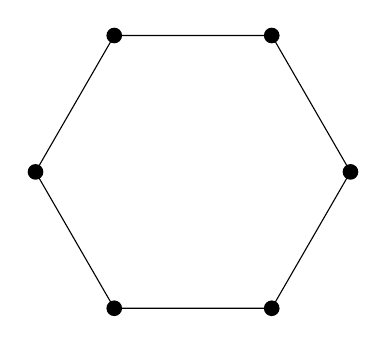
\begin{tikzpicture}
            % Defining the vertices of the cycle
            \foreach \x in {0,60,...,300} {
                    \node[circle, fill=black, inner sep=2pt] at (\x:2) {};
                }
            % Drawing the edges of the cycle
            \draw (0:2) -- (60:2) -- (120:2) -- (180:2) -- (240:2) -- (300:2) -- cycle;
        \end{tikzpicture}
    \end{center}

    Da minimiziramo \(\frac{\abs{\partial S}}{\abs{S}}\) lahko vzamemo sosednja vozlišča. Tako bo vedno \(\abs{\partial S} = 2\), \(S\) pa povečamo do polovice cikla, kot omejuje definicija. Za cikel \(C_{2n}\) torej vzamemo \(\abs{S} = n\), za \(C_{2n+1}\) pa prav tako \(\abs{S} = n\).
    \begin{align*}
        c(C_n) = \frac{2}{\lfloor \frac n2\rfloor}
    \end{align*}
    Večji kot je \(n\), manjša je Cheegerjeva konstanta in graf je slabše povezan, saj rabimo odstraniti le dve povezavi da ločimo veliko vozlišč od preostanka.
\end{primer}
\begin{primer}[Polni grafi]
    \hspace{0em}
    \begin{center}
        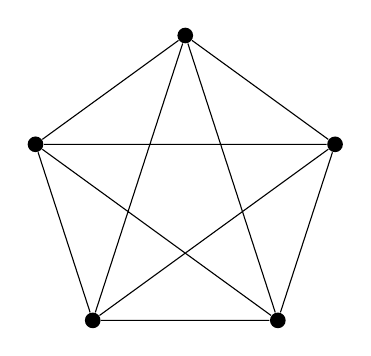
\begin{tikzpicture}
            \node[circle, fill=black, inner sep=2pt] (A) at (90:2) {};
            \node[circle, fill=black, inner sep=2pt] (B) at (162:2) {};
            \node[circle, fill=black, inner sep=2pt] (C) at (234:2) {};
            \node[circle, fill=black, inner sep=2pt] (D) at (306:2) {};
            \node[circle, fill=black, inner sep=2pt] (E) at (18:2) {};
            \draw (A) -- (B) -- (C) -- (D) -- (E) -- (A);
            \draw (A) -- (C) -- (E) -- (B) -- (D) -- (A);
        \end{tikzpicture}
    \end{center}
    Za graf \(K_n\) velja, da je \(\abs{\partial S} = \abs{S} \cdot (n - \abs{S})\). Torej je
    \begin{align*}
        c(K_n) = \min_{S} n-\abs{S}
    \end{align*}
    minimum je dosežen pri \(\abs{S} = \lfloor\frac n2\rfloor\) s poljubno izbiro vozlišč.
    \begin{align*}
        c(K_n) = \left\lceil \frac n2 \right\rceil
    \end{align*}
    Večji kot je \(n\), večja je Cheegerjeva konstanta in graf je bolje povezan.
\end{primer}
Oglejmo si še primer, kjer je zelo očitna povezava med ozkim grlom grafa in Cheegerjevo konstanto.
\begin{primer}[Ozko grlo]\hspace{0em}
    \begin{figure}
        \centering
        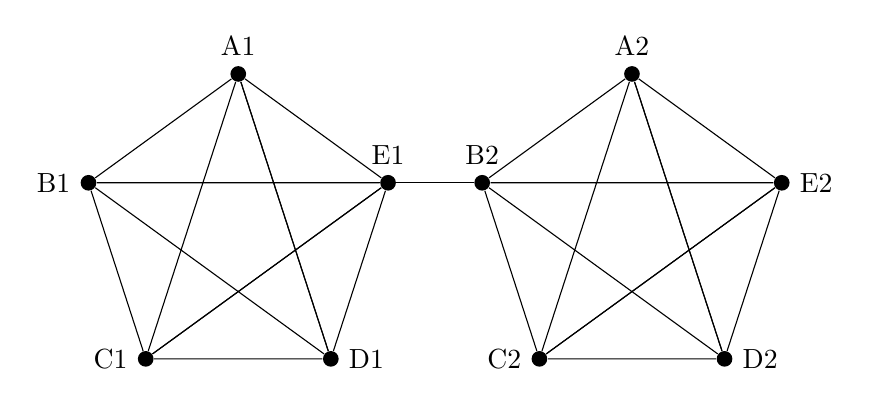
\begin{tikzpicture}
            % First K_5
            \begin{scope}[shift={(0,0)}]
                \node[circle, fill=black, inner sep=2pt, label=above:A1] (A1) at (90:2) {};
                \node[circle, fill=black, inner sep=2pt, label=left:B1] (B1) at (162:2) {};
                \node[circle, fill=black, inner sep=2pt, label=left:C1] (C1) at (234:2) {};
                \node[circle, fill=black, inner sep=2pt, label=right:D1] (D1) at (306:2) {};
                \node[circle, fill=black, inner sep=2pt, label=above:E1] (E1) at (18:2) {};
                \draw (A1) -- (B1) -- (C1) -- (D1) -- (E1) -- (A1);
                \draw (A1) -- (C1) -- (E1) -- (B1) -- (D1) -- (A1);
                \draw (A1) -- (D1);
                \draw (B1) -- (E1);
                \draw (C1) -- (E1);
            \end{scope}

            % Second K_5
            \begin{scope}[shift={(5,0)}]
                \node[circle, fill=black, inner sep=2pt, label=above:A2] (A2) at (90:2) {};
                \node[circle, fill=black, inner sep=2pt, label=above:B2] (B2) at (162:2) {};
                \node[circle, fill=black, inner sep=2pt, label=left:C2] (C2) at (234:2) {};
                \node[circle, fill=black, inner sep=2pt, label=right:D2] (D2) at (306:2) {};
                \node[circle, fill=black, inner sep=2pt, label=right:E2] (E2) at (18:2) {};
                \draw (A2) -- (B2) -- (C2) -- (D2) -- (E2) -- (A2);
                \draw (A2) -- (C2) -- (E2) -- (B2) -- (D2) -- (A2);
                \draw (A2) -- (D2);
                \draw (B2) -- (E2);
                \draw (C2) -- (E2);
            \end{scope}

            % Connecting edge between the two K_5 graphs
            \draw (E1) -- (B2);
        \end{tikzpicture}
        \caption{Povezana grafa \(K_5\)}
    \end{figure}
    Dvem polnim grafom \(K_n\) dodamo povezavo, da dobimo povezan graf \(G = (V,E)\). Če za \(S\) vzamemo enega izmed polnih grafov, je \(\abs{S} = n\) maksimalen in \(\abs{\partial S} = 1\) minimalen. Torej je Cheegerjeva konstanta
    \begin{align*}
        c(G) = \frac{1}{n}.
    \end{align*}
    Večji kot je \(n\), bolj izrazito je ozko grlo na grafu, kar vidimo tudi v manjši \(c(G)\).
\end{primer}
\subsection{Spektralna vrzel}
Graf lahko predstavimo tudi s sosednostno matriko. Vozlišča grafa \(G=(V,E)\) označimo od \(1\) do \(n=\abs{V}\) in naredimo \(n\times n\) matriko \(N(G)\), ki ima vrednost \(1\) na \((i,j)\)-tem mestu, če obstaja povezava med vozliščem \(i\) in \(j\) (oziroma \((i,j)\in E\)). Če povezave ni, je na tistem mestu vrednost \(0\).

Ker so grafi neusmerjeni je matrika simetrična. Po spektralnem izreku ima torej \(n\) realnih lastnih vrednosti \(\lambda_i\), ki jih uredimo po velikosti.
\begin{align*}
    \lambda_1 \geq \lambda_2 \geq \ldots \geq \lambda_n
\end{align*}

\begin{definicija}[Spektralna vrzel]
    Spektralna vrzel grafa \(G\) je razlika med dvema največjima lastnima vrednostima njegove sosednostne matrike.
    \begin{align*}
        s(G) = \lambda_1 - \lambda_2
    \end{align*}
\end{definicija}
\begin{primer}[Cikli]
    Graf \(C_n\) ima sosednostno matriko
    \begin{align*}
        N(C_n) = \begin{bmatrix}
                     0      & 1      & 0      & 0      & \cdots & 0      & 0      & 1      \\
                     1      & 0      & 1      & 0      & \cdots & 0      & 0      & 0      \\
                     0      & 1      & 0      & 1      & \cdots & 0      & 0      & 0      \\
                     \vdots & \vdots & \vdots & \vdots & \ddots & \vdots & \vdots & \vdots \\
                     0      & 0      & 0      & 0      & \cdots & 1      & 0      & 1
                 \end{bmatrix}.
    \end{align*}
    Matrika je cirkulantna, zato poznamo njene lastne vrednosti.
    \begin{align*}
        \lambda(N(C_n)) = \left\{ 2 \cos\left(\frac{2\pi k}{n}\right) \mid 0 \leq k \leq n-1\right\}
    \end{align*}
    % Add source?
    Od tod sledi, da je spektralna vrzel
    \begin{align*}
        s(C_n) = 2 - 2\cos\frac{2\pi}{n}.
    \end{align*}
    Opazimo da večji kot je graf, manjša je spektralna vrzel, prav tako kot je manjša Cheegerjeva konstanta.
\end{primer}
\begin{primer}[Polni grafi]
    Graf \(K_n\) ima sosednostno matriko
    \begin{align*}
        N(K_n) = \begin{bmatrix}
                     0      & 1      & 1      & \cdots & 1      \\
                     1      & 0      & 1      & \cdots & 1      \\
                     1      & 1      & 0      & \cdots & 1      \\
                     \vdots & \vdots & \vdots & \ddots & \vdots \\
                     1      & 1      & 1      & \cdots & 0
                 \end{bmatrix}.
    \end{align*}
    Lastne vrednosti matrike dobimo tako, da uganemo lastne vektorje.
    \begin{align*}
        v_1 = \begin{bmatrix}
                  1      \\
                  1      \\
                  \vdots \\
                  1
              \end{bmatrix} \\
        N(K_n) v_1 = (n-1) \cdot v_1
    \end{align*}
    Torej je ena lastna vrednost \(n-1\). Ostale lastne vektorje \(v_j\) za \(j>1\) dobimo kot
    \begin{align*}
        v_j = e_1 - e_j,
    \end{align*}
    kjer je \(e_j\) enotski vektor z \(1\) v \(j\)-ti komponenti. Ker je
    \begin{align*}
        N(K_n)v_j = -1 \cdot v_j,
    \end{align*}
    dobimo še \(n-1\) lastnih vrednosti \(-1\). Spektralna vrzel je torej
    \begin{align*}
        s(K_n) = (n-1) - (-1) = n.
    \end{align*}
    Opazimo da večji kot je graf, večja je vrzel (prav tako, kot je večja Cheegerjeva konstanta).
\end{primer}
\begin{primer}[Ozko grlo]
    Vzamemo primer dveh grafov \(K_n\), povezanih z eno povezavo. Matrika sosednosti je dimenzije \(2n \times 2n\) in ima na zgornji levi \(n\times n\) podmatriki vrednosti \(1\) povsod razen na diagonali, kjer so vrednosti \(0\). Enako je na spodnji desni \(n\times n\) podmatriki (tako dobimo dva grafa \(K_n\) kot podgrafa). Ostale vrednosti so \(0\), razen na elementu matrike \((1, n+1)\) in \((n+1, 1)\), kjer je vrednost \(1\) (ki predstavlja povezavo med grafoma \(K_n\)).

    Spektralne vrzeli izračunamo numerično in izrišemo na grafu.
    % compute/definicije_spectral_gap_bottleneck.py
    \begin{figure}[h!]
        \centering
        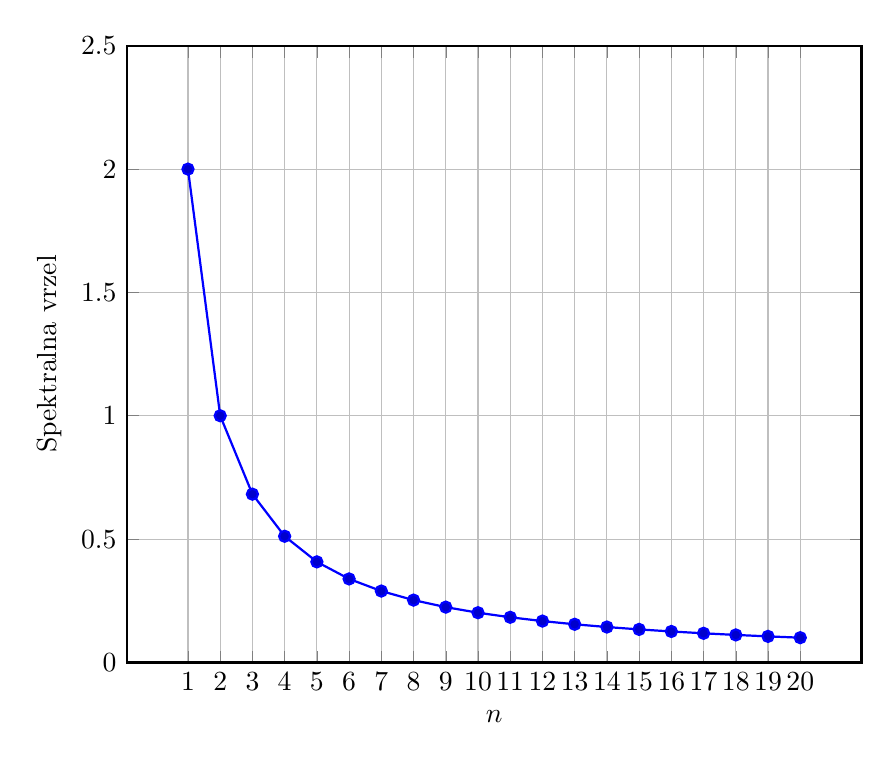
\begin{tikzpicture}
            \begin{axis}[
                    xlabel={$n$},
                    width=0.9\textwidth,
                    ylabel={Spektralna vrzel},
                    grid=major,
                    ymin=0, ymax=2.5,
                    xtick={1,2,...,20},
                    ytick={0,0.5,1,1.5,2,2.5},
                    thick
                ]
                \addplot coordinates {
                        (1, 2.0)
                        (2, 0.9999999999999988)
                        (3, 0.6821627548042195)
                        (4, 0.5114877902540731)
                        (5, 0.40764085275359996)
                        (6, 0.3384804373175667)
                        (7, 0.28929431396096117)
                        (8, 0.2525727509441946)
                        (9, 0.22412614005130305)
                        (10, 0.20144531545046007)
                        (11, 0.18293973049316747)
                        (12, 0.16755365441690628)
                        (13, 0.15455930002271145)
                        (14, 0.14343884532369877)
                        (15, 0.13381387867170424)
                        (16, 0.1254014671437087)
                        (17, 0.11798583829938813)
                        (18, 0.11139957046625426)
                        (19, 0.10551076707121965)
                        (20, 0.10021410708796452)
                    };
            \end{axis}
        \end{tikzpicture}
        \caption{Graf spektralnih vrzeli za \(n\) od 1 do 20}
    \end{figure}
    Opazimo, da večji kot je \(n\), manjša je spektralna vrzel, prav tako kot je manjša Cheegerjeva konstanta (in bolj kot je očitno ozko grlo).
\end{primer}

Računanje lastnih vrednosti regularnega grafa nam olajša tudi lastnost, da je njegova največja lastna vrednost enaka stopnji regularnosti.
\begin{izrek}[Največja vrednost \(d\)-regularnega grafa]
    Največja lastna vrednost \(d\)-regularnega grafa je \(d\).
\end{izrek}
\begin{dokaz}
    Lastni vektor \(d\)-regularnega grafa \(G\) za lastno vrednost \(d\) je vedno vektor samih enic, saj ima vsaka vrstica sosednostne matrike natanko \(n\) enic.

    Večje lastne vrednosti ne obstaja, saj so elementi sosednostne matrike samo \(0\) in \(1\). Če bi obstajala lastna vrednost \(\lambda > d\), potem si ogledamo največji element lastnega vektorja za to lastno vrednost, \(x\). Ker ima matrika natanko \(d\) enic v vsaki vrstici (in ostale vrednosti \(0\)), bi moralo obstajati \(d\) elementov vektorja, ki se skupaj sešteje v \(\lambda x\). Ker pa je vsak element manjši ali enak \(x\), imamo jih pa \(d\) lahko dosežemo kvečjemu \(d \times x\), torej večja lastna vrednost ne obstaja.
\end{dokaz}
Če je graf regularen torej, potrebujemo le izračunati njegovo drugo največjo lastno vrednost.
\subsection{Cheegerjeva neenakost}
Opazili smo, da se Cheegerjeva konstanta in spektralna vrzel obnašata podobno. Definiciji pa nista enakovredni - obstajajo na primer grafi, kjer lahko dodamo povezave ampak znižamo spektralno vrzel (medtem, ko bo Cheegerjeva konstanta ne more postati nižja).

\begin{primer}[Dodajanje povezave poviša vrzel]
    % compute/edges_increase_gap.py
    Kot primer vzamemo graf
    % change the labels to be as in the bottleneck example. Also make h! work
    \begin{figure}[h!]
        \centering
        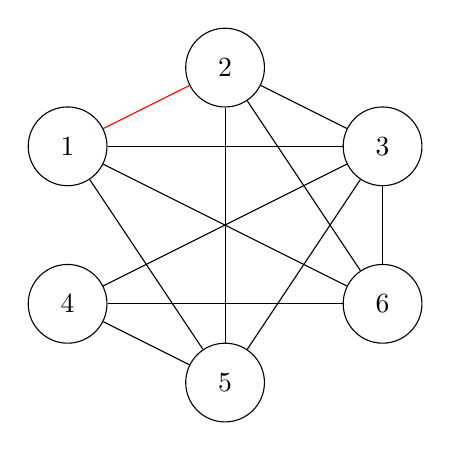
\begin{tikzpicture}[scale=1, every node/.style={circle, draw, minimum size=1cm}]
            % Nodes
            \node (1) at (0,2) {1};
            \node (2) at (2,3) {2};
            \node (3) at (4,2) {3};
            \node (4) at (0,0) {4};
            \node (5) at (2,-1) {5};
            \node (6) at (4,0) {6};

            % Edges based on the adjacency matrix
            \path[draw=red] (1) edge (2);
            \path (1) edge (3);
            \path (1) edge (5);
            \path (1) edge (6);

            \path (2) edge (3);
            \path (2) edge (5);
            \path (2) edge (6);

            \path (3) edge (4);
            \path (3) edge (5);
            \path (3) edge (6);

            \path (4) edge (5);
            \path (4) edge (6);
        \end{tikzpicture}
    \end{figure}
    s sosednostno matriko
    \begin{align*}
        \begin{bmatrix}
            0          & \mathbf{1} & 1 & 0 & 1 & 1 \\
            \mathbf{1} & 0          & 1 & 0 & 1 & 1 \\
            1          & 1          & 0 & 1 & 1 & 1 \\
            0          & 0          & 1 & 0 & 1 & 1 \\
            1          & 1          & 1 & 1 & 0 & 0 \\
            1          & 1          & 1 & 1 & 0 & 0 \\
        \end{bmatrix}.
    \end{align*}
    Spektralna vrzel grafa je približno \(3.706\), če pa odstranimo povezavo med vozliščema \(1\) in \(2\) dobimo spektralno vrzel približno \(3.766\). Tako smo graf naredili slabše povezanega, spektralno vrzel pa vseeno povišali. Cheegerjeva konstanta pa je v obeh primerih enaka \(2\) (kjer za \(S\) lahko vzamemo vozlišča \(1\), \(2\) in \(5\)).
\end{primer}

Kljub temu pa lahko povezavo med konceptoma Cheegerjeve neenakosti in spektralne vrzeli vseeno formaliziramo.
\begin{izrek}[Cheegerjeva neenakost]
    Za \(d\)-regularen graf \(G\) velja 
    \begin{align*}
        \frac{1}{2}s(G) \leq c(G) \leq \sqrt{2ds(G)}
    \end{align*}
    oziroma
    \begin{align*}
        2c(G) \geq s(G) \geq \frac{c(G)^2}{2d}
    \end{align*}    
\end{izrek}
Za dokaz izreka potrebujemo naslednjo lemo.
\begin{lema}\label{cheegerLema}
    Za poljubna \(a, b, c, d > 0\) velja
    \begin{align*}
        \frac{a+b}{c+d} \geq \min\left(\frac{a}{c}, \frac{b}{d}\right).
    \end{align*}
\end{lema}
\begin{dokaz}
    \begin{align*}
        a+b &= c\cdot\frac{a}{c} + d\cdot \frac{a}{d}\\
        a+b &\geq (c+d) \min\left(\frac{a}{c}, \frac{b}{d}\right)\\
        \frac{a+b}{c+d} &\geq \min\left(\frac{a}{c}, \frac{b}{d}\right)
    \end{align*}
\end{dokaz}
\begin{dokaz}[Dokaz Cheegerjeve neenakosti]
    Dokažimo najprej \(2c(G) \geq s(G)\). Naj bo \(S\subset V(G)\) tak, da zadosti minimumu iz definicije Cheegerjeve konstante, torej \(0<\abs{S} \leq \frac12\abs{V(G)}\) in 
    \begin{align*}
        c(G) = \frac{\abs{\partial S}}{\abs{S }}.
    \end{align*}
    Spektralno vrzel poiščemo prek Rayleighovega kvocienta. Če je \(A\) sosednostna matrika grafa je Rayleighov kvocient
    \begin{align*}
        R(A, v) = \frac{v^\top Av}{v^\top v}.
    \end{align*}
    Vemo že, da je vektor samih enic lastni vektor sosednostne matrike za največjo lastno vrednost \(d\). Če torej želimo drugo največjo lastno vrednost, lahko poiščemo maksimum Rayleighovega kvocienta po vseh vektorjih, ki so pravokotni na vektor samih enic. Da pokažemo želeno neenakost izberemo specifičen vektor \(v\) in izračunamo njegov Rayleighov kvocient. Druga največja lastna vrednost bo večja ali enaka od izračunanega kvocienta, spektralna vrzel pa zato manjša.

    Izberemo vektor \(v\) tako, da ima elemente enake \(\frac{1}{\abs{S}}\) na indeksih, ki pripadajo elementom iz \(S\) ter ostale elemente (tiste, ki pripadajo indeksom za \(\overline S\)) enake \(-\frac{1}{\abs{\overline S}}\). Ta vektor je pravokoten na vektor samih enic.
    Sedaj izračunamo Rayleighov kvocient.
    \begin{align*}
        Av = \left(\sum_{j=1}^{\abs{V(G)}} v_j \cdot A_{i,j}\right)_{i=1}^{\abs{V(G)}}\\
        v^\top Av = \sum_{i=1}^{\abs{V(G)}} \sum_{j=1}^{\abs{V(G)}} v_i v_j A_{i,j} = \sum_{i\sim j} v_i v_j\\
    \end{align*}
    \begin{align*}
        R(A, v) &= \frac{\sum_{i\sim j} v_i v_j}{\sum_{i=1}^{\abs{V(G)}}v_i^2}\\
        &= \frac{\sum_{i\sim j} v_i^2 + v_j^2 - \left(v_i - v_j\right)^2}{2 \sum_{i=1}^{\abs{V(G)}}v_i^2}\\
        &= \frac{\sum_{i\sim j} v_i^2}{\sum_{i=1}^{\abs{V(G)}}v_i^2} - \frac{\sum_{i\sim j}\left(v_i - v_j\right)^2}{2 \sum_{i=1}^{\abs{V(G)}}v_i^2}\\
        &= \frac{d\cdot \sum_{i=1}^{\abs{V(G)}}v_i^2}{\sum_{i=1}^{\abs{V(G)}}v_i^2} -  \frac{2\cdot \sum_{i\in S \land j \in \overline S}\left(v_i - v_j\right)^2}{2 \sum_{i=1}^{\abs{V(G)}}v_i^2}\\
        &= d - \frac{\abs{\partial S} \cdot \left(\frac{1}{\abs{S}} + \frac{1}{\abs{\overline S}}\right)^2}{\abs{S} \frac{1}{\abs{S}^2} + \abs{\overline S} \frac{1}{\abs{\overline S}^2}}\\
        &= d - \abs{\partial S}\left(\frac{1}{\abs{S}} + \frac{1}{\abs{\overline S}}\right) \\ 
        &= d - \frac{\abs{\partial S}}{\abs{S}}\frac{\left(\abs{S} + \abs{\overline S}\right)}{\abs{\overline S}}\\
        &= d- c(G) \frac{V(G)}{\abs{\overline S}}\\
        &\geq d - 2c(G)
    \end{align*}
    Torej velja
    \begin{align*}
        \lambda_2 \geq R(A,v) \geq d-2c(G)\\
        2c(G) \geq d-\lambda_2 = s(G)
    \end{align*}

    % file:///home/tadej/library/math/magistrska/cheeger_chung.pdf
    Sedaj dokažemo še drugo neenakost, \(s(G) \geq \frac{c(G)^2}{2d}\). Tu bomo preko Fiedlerjevega algoritma s pomočjo lastnega vektorja za drugo največjo lastno vrednost konstruirali particijo grafa.

    Naj bo \(v\) lastni vektor za drugo največjo lastno vrednost, \(\lambda_2\). Brez škode za splošnost preuredimo vozlišča grafa tako, da je \(v_i \geq v_j\) za \(i < j\). Definiramo \(S_i = \{v_1, \ldots, v_i\}\) in 
    \begin{align*}
        \alpha(G) = \min_{1\leq i \leq V(G)/2} \frac{\abs{\partial S_i}}{\abs{S_i}}.
    \end{align*}
    Očitno je \(h(G) \leq \alpha(G)\).

    Vzamemo \(r=\floor{\frac{V(G)}{2}}\) in definiramo
    \begin{align*}
        v^+_i = \begin{cases}
            v_i - v_r & v_i \geq v_r \\
            0 & v_i < v_r
        \end{cases}\\
        v^-_i = \begin{cases}
            v_r - v_i & v_i \leq v_r \\
            0 & v_i > v_r
        \end{cases}.
    \end{align*}
    Predpostavimo, da velja \(R(A, v^+) \geq R(A, v^-)\), sicer lastni vektor \(v\) pomnožimo z \(-1\). Izbrali smo \(r\) tako, da bosta vedno oba vektorja (\(v^+\) in \(v^-\)) imela kvečjemu \(r\) pozitivnih elementov, kar se ohrani, če zamenjamo predznake v vektorju \(v\), kot zahteva predpostavka. Vozlišča, ki pripadajo pozitivnim elementom \(v^+\) bomo uporabili pri vpeljavi \(\alpha(G)\), ki pa zahteva podgraf velikosti največ \(r\). Predpostavko lahko zapišemo tudi drugače:
    \begin{align}\label{eq:cheegerPredpostavka}
        \frac{\sum_{i\sim j}(v^+_i - v^+_j)^2}{2\sum_{i=1}^{\abs{V(G)}} (v^+_i)^2} \leq \frac{\sum_{i\sim j} (v^-_i - v^-_j)^2}{2\sum_{i=1}^{\abs{V(G)}} (v^-_i)^2} 
    \end{align}

    Podobno kot v prvem delu dokaza preko Rayleighovega kvocienta izrazimo spektralno luknjo.
    \begin{align*}
        s(G) &= d-\lambda_2 \\ 
        &= \frac{\sum_{i\sim j}(v_i - v_j)^2}{2\sum_{i=1}^{\abs{V(G)}} v_i^2}
    \end{align*}
    
    Ker je \(v\) pravokoten na največji lastni vektor, vektor samih enic, velja \(\sum_i v_i = 0\). Tako lahko povečamo imenovalec kvocienta:
    \begin{align*}
        \sum_{i=1}^{\abs{V(G)}} v_i^2 = \min_{c\in \R} \sum_{i=1}^{\abs{V(G)}} (v_i - c)^2 \leq \sum_{i=1}^{\abs{V(G)}} (v_i - v_r)^2\\
        \frac{\sum_{i\sim j}(v_i - v_j)^2}{2\sum_{i=1}^{\abs{V(G)}} v_i^2} \geq \frac{\sum_{i\sim j}(v_i - v_j)^2}{2\sum_{i=1}^{\abs{V(G)}} (v_i-v_r)^2}
    \end{align*}
    Imenovalec lahko prepišemo z uporabo \(v^+\) in \(v^-\)
    \begin{align*}
        \frac{\sum_{i\sim j}(v_i - v_j)^2}{2\sum_{i=1}^{\abs{V(G)}} v_i^2} \geq \frac{\sum_{i\sim j}(v_i - v_j)^2}{2\sum_{i=1}^{\abs{V(G)}} (v_i-v_r)^2} = \frac{\sum_{i\sim j}(v_i - v_j)^2}{2\sum_{i=1}^{\abs{V(G)}} (v^+_i)^2 + 2\sum_{i=1}^{\abs{V(G)}} (v^-_i)^2}.
    \end{align*}
    
    Sedaj pomanjšamo števec \(\sum_{i\sim j}(v_i - v_j)^2\). Če sta \(v_i\) in \(v_j\) oba večja od \(v_r\), potem velja
    \begin{align*}
        (v_i - v_j)^2 = (v^+_i - v^+_j)^2 + (v^-_i - v^-_j)^2.
    \end{align*}
    Enako velja, če sta oba manjša od \(v_r\). V primeru ko je \(v_j \leq v_r \leq v_i\), pa vidimo slednje:
    \begin{align*}
        0 \geq (v_r - v_i)(v_r - v_j)\\
        0 \geq v_r^2 - v_r v_i - v_r v_j + v_i v_j \\
        -2 v_i v_j \geq 2 v_r^2 - 2 v_r v_i - 2 v_r v_j \\
        v_i^2 - 2v_i v_j + v_j^2 \geq (v_r^2 - 2v_r v_i + v_i^2) + (v_r^2 - 2v_r v_j + v_j^2) \\ 
        (v_i - v_j)^2 \geq (v_i - v_r -0)^2 + (0 + v_j - v_r)^2 \\
        (v_i - v_j)^2 \geq  (v^+_i - v^+_j)^2 + (v^-_i - v^-_j)^2
    \end{align*}
    Enako velja v primeru \(v_i \leq v_r \leq v_j\), torej je
    \begin{align*}
        s(G) &\geq \frac{\sum_{i\sim j}(v_i - v_j)^2}{2\sum_{i=1}^{\abs{V(G)}} (v^+_i)^2 + 2\sum_{i=1}^{\abs{V(G)}} (v^-_i)^2}\\
        &\geq \frac{\sum_{i\sim j}(v^+_i - v^+_j)^2 + (v^-_i - v^-_j)^2}{2\sum_{i=1}^{\abs{V(G)}} (v^+_i)^2 + 2\sum_{i=1}^{\abs{V(G)}} (v^-_i)^2}
    \end{align*}
    
    Zgornjo neenakost lahko, s pomočjo predpostavke \eqref{eq:cheegerPredpostavka} in leme \ref{cheegerLema} spremenimo v

    \begin{align*}
        s(G) \geq  \frac{\sum_{i\sim j}(v^+_i - v^+_j)^2}{2\sum_{i=1}^{\abs{V(G)}} (v^+_i)^2}.
    \end{align*}
    Od tod sledi
    \begin{align*}
        s(G) &\geq  \frac{\sum_{i\sim j}(v^+_i - v^+_j)^2}{2\sum_{i=1}^{\abs{V(G)}} (v^+_i)^2} \frac{\sum_{i\sim j}(v^+_i + v^+_j)^2}{\sum_{i\sim j}(v^+_i + v^+_j)^2}\\
        &= \frac{\sum_{i\sim j}(v^+_i - v^+_j)^2}{2\sum_{i=1}^{\abs{V(G)}} (v^+_i)^2} \frac{\sum_{i\sim j}(v^+_i + v^+_j)^2}{\sum_{i\sim j}(v^+_i)^2 + (v^+_j)^2 + 2v^+_i v^+_j}\\
        &= \frac{\sum_{i\sim j}(v^+_i - v^+_j)^2}{2\sum_{i=1}^{\abs{V(G)}} (v^+_i)^2} \frac{\sum_{i\sim j}(v^+_i + v^+_j)^2}{2d\sum_{i=1}^{\abs{V(G)}} (v^+_i)^2 + 2\sum_{i\sim j}v^+_i v^+_j}
    \end{align*}
    Uporabimo Cauchy-Schwarzovo neenakost ločeno na števcu in na delu imenovalca.
    \begin{align*}
        s(G) &\geq  \frac{\left(\sum_{i\sim j}(v^+_i - v^+_j)(v^+_i + v^+_j)\right)^2}{2\sum_{i=1}^{\abs{V(G)}} (v^+_i)^2\left(2d\sum_{i=1}^{\abs{V(G)}} (v^+_i)^2 + 2\sqrt{\sum_{i\sim j}(v^+_i)^2 \sum_{i\sim j} (v^+_j)^2}\right)}\\
        &= \frac{\left(\sum_{i\sim j}\abs{(v^+_i)^2 - (v^+_j)^2} \right)^2}{2\sum_{i=1}^{\abs{V(G)}} (v^+_i)^2 \left(2d\sum_{i=1}^{\abs{V(G)}} (v^+_i)^2 + 2d \sum_{i=1}^{\abs{V(G)}}(v^+_i)^2 \right)}\\
        &= \frac{\left(\sum_{i\sim j}\abs{(v^+_i)^2 - (v^+_j)^2} \right)^2}{8d\left(\sum_{i=1}^{\abs{V(G)}} (v^+_i)^2\right)^2}\\
        &= \frac{\left(2\sum_{i\sim j \land i< j}(v^+_i)^2 - (v^+_j)^2 \right)^2}{8d\left(\sum_{i=1}^{\abs{V(G)}} (v^+_i)^2\right)^2} \\
        &= \frac{\left(\sum_{i\sim j \land i< j}(v^+_i)^2 - (v^+_j)^2 \right)^2}{2d\left(\sum_{i=1}^{\abs{V(G)}} (v^+_i)^2\right)^2}
    \end{align*}
    Vsak sumand \((v^+_i)^2 - (v^+_j)^2\) lahko teleskopsko razpišemo kot
    \begin{align*}
        (v^+_i)^2 &- (v^+_{i+1})^2\\
        + (v^+_{i+1})^2 &- (v^+_{i+2})^2\\
        + &\cdots\\
        + (v^+_{j-1})^2 &- (v^+_{j})^2,
    \end{align*}
    da dobimo
    \begin{align*}
        s(G) &\geq \frac{\left(\sum_{i=1}^{\abs{V(G)}}\abs{\partial S_i}\left((v^+_i)^2 - (v^+_{i+1})^2\right) \right)^2}{2d\left(\sum_{i=1}^{\abs{V(G)}} (v^+_i)^2\right)^2}
        &=\frac{\left(\sum_{i=1}^{r}\abs{\partial S_i}\left((v^+_i)^2 - (v^+_{i+1})^2\right) \right)^2}{2d\left(\sum_{i=1}^{r} (v^+_i)^2\right)^2}
    \end{align*}
    Po definiciji za vsak \(i\leq r\) velja \(\abs{\partial S_i} \geq \abs{S_i} \alpha(G)\).
    \begin{align*}
        s(G) &\geq \frac{\left(\sum_{i=1}^{r} \abs{S_i} \alpha(G)\left((v^+_i)^2 - (v^+_{i+1})^2\right) \right)^2}{2d\left(\sum_{i=1}^{r} (v^+_i)^2\right)^2}\\
        &= \frac{\alpha(G)^2}{2d} \frac{\left(\sum_{i=1}^{r} \abs{S_i}\left((v^+_i)^2 - (v^+_{i+1})^2\right) \right)^2}{\left(\sum_{i=1}^{r} (v^+_i)^2\right)^2}\\
        &= \frac{\alpha(G)^2}{2d} \frac{\left(\sum_{i=1}^{r} i\cdot (v^+_i)^2 - \sum_{i=1}^{r} (i-1) \cdot (v^+_{i})^2 \right)^2}{\left(\sum_{i=1}^{r} (v^+_i)^2\right)^2}\\
        &= \frac{\alpha(G)^2}{2d} \frac{\left(\sum_{i=1}^{r} i\cdot (v^+_i)^2 - \sum_{i=1}^{r} (i-1) \cdot (v^+_{i})^2 \right)^2}{\left(\sum_{i=1}^{r} (v^+_i)^2\right)^2}\\
        &= \frac{\alpha(G)^2}{2d} \frac{\left(\sum_{i=1}^{r} \cdot (v^+_i)^2 \right)^2}{\left(\sum_{i=1}^{r} (v^+_i)^2\right)^2}\\
        &= \frac{\alpha(G)^2}{2d}\\
    \end{align*}
    Tako dobimo
    \begin{align*}
        s(G) \geq \frac{\alpha(G)^2}{2d} \geq \frac{h(G)^2}{2d}
    \end{align*}



\end{dokaz}
\subsection{Alon-Boppanov izrek}
\subsection{Ramanujanovi grafi}

%%%%%%%%%%%%%%%%%%%%%%%%%%%%%%%%%%%%%%%%%%%%%%%%%%%%%%%%%%%%%%%%%%%%%%%%%%%%%%%
% ZAČETEK VSEBINE
%%%%%%%%%%%%%%%%%%%%%%%%%%%%%%%%%%%%%%%%%%%%%%%%%%%%%%%%%%%%%%%%%%%%%%%%%%%%%%%

\begin{document}

\section{Uvod}
Grafi so ena izmed najbolj uporabnih struktur v matematiki. Služijo kot orodje pri reševanju problemov v drugih vejah matematike, kot pripomoček za modeliranje realnih situacij ali pa jih preučujemo kot samostojen matematični koncept. Pogosto potrebujemo grafe, ki imajo visoko količino povezav.

Poglejmo konkreten primer iz vsakdanjega življenja. Vozlišča v grafu naj predstavljajo mesta, povezave med njimi pa ceste, ki vodijo med mesti. Želimo si, da bi bilo mogoče iz vsakega mesta potovati do katerega koli drugega mesta. To drži natanko tedaj, ko je graf povezan. Lahko pa bi se zgodilo, da neka cesta postane neprevozna, na primer zaradi prometne nesreče ali naravne katastrofe. To predstavimo tako, da odstranimo povezavo v grafu. V hujših primerih bi lahko prišlo do uničenja več cest. Kljub temu želimo, da naš graf ostane povezan ter tako lahko še vedno potujemo med mesti in je naša infrastruktura bolj odporna proti motnjam. Najbolj robustno bi bilo omrežje, v katerem bi bilo vsako mesto povezano z vsemi ostalimi, vendar bi bilo to predrago, zato si želimo, da je število povezav majhno, še vedno pa jih potrebujemo odstraniti veliko, preden graf postane nepovezan.
Podoben primer najdemo v električnih omrežjih, kjer vozlišča predstavljajo transformatorske postaje, povezave pa daljnovode med njimi. Lahko bi pa za vozlišča uporabljali usmerjevalnike ter za povezave internetne kable. V vseh primerih želimo dobiti čim bolj odporno omrežje za čim manjšo ceno infrastrukture. Ramanujanovi grafi so grafi, ki so na nekakšen način optimalni glede na opisano metriko.

\section{Ramanujanovi grafi}
Koncept ramanujanovih grafov ima enostavno definicijo, vendar njen pomen ni očiten brez predhodne motivacije s sorodnimi definicijami in izreki. Te nam razjasnijo povezavo med lastnimi vrednostmi grafa, ki se pojavijo v definiciji Ramanujanovih grafov, ter povezljivostjo grafa.
\subsection{Cheegerjeva konstanta}
Kot v uvodnem primeru nas zanima koliko povezav moremo odstraniti, da graf ni več povezan.

Naj bo \(G=(V,E)\) povezan graf in \(S\subseteq V\) podmnožica vozlišč z \(0<\abs{S} \leq \frac{\abs{V}}{2}\). Z \(\partial S\subseteq E\) označimo množico povezav od \(S\) do komplementa vozlišč, \(\overline{S}\). Če iz grafa odstranimo \(\partial S\), potem se graf postane nepovezan.

Najbolj problematična so ozka grla grafa. To je majhna množica povezav, ki ločuje dva dela grafa z veliko vozlišči. Da je graf dobro povezan torej želimo, da ni ozkih grl in da je za velik \(\abs{S}\) tudi velik \(\abs{\partial S} \), oziroma da \(\frac{\abs{S}}{\abs{\partial S}}\) ni nikoli majhen.

% reword T?
\begin{definicija}[Cheegerjeva konstanta]
    Za graf \(G = (V,E)\) in njegova vozlišča \(T = \left\{S\subseteq V \mid 0<\abs{S} \leq \frac{\abs{V}}{2}\right\}\) definiramo Cheegerjevo konstanto kot
    \begin{align*}
        c(G) = \min_{S\in T} \frac{\abs{\partial S}}{\abs{S}}
    \end{align*}
\end{definicija}
Večji kot je \(c(G)\), manj ozkih grl ima graf \(G\).

\begin{primer}[Cikli]
    \hspace{0em}
    \begin{center}
        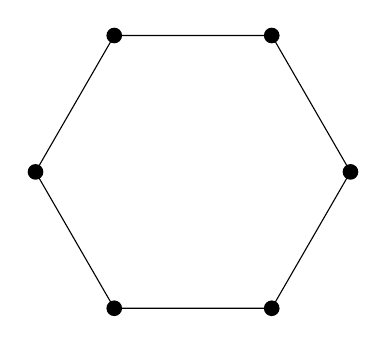
\begin{tikzpicture}
            % Defining the vertices of the cycle
            \foreach \x in {0,60,...,300} {
                    \node[circle, fill=black, inner sep=2pt] at (\x:2) {};
                }
            % Drawing the edges of the cycle
            \draw (0:2) -- (60:2) -- (120:2) -- (180:2) -- (240:2) -- (300:2) -- cycle;
        \end{tikzpicture}
    \end{center}

    Da minimiziramo \(\frac{\abs{\partial S}}{\abs{S}}\) lahko vzamemo sosednja vozlišča. Tako bo vedno \(\abs{\partial S} = 2\), \(S\) pa povečamo do polovice cikla, kot omejuje definicija. Za cikel \(C_{2n}\) torej vzamemo \(\abs{S} = n\), za \(C_{2n+1}\) pa prav tako \(\abs{S} = n\).
    \begin{align*}
        c(C_n) = \frac{2}{\lfloor \frac n2\rfloor}
    \end{align*}
    Večji kot je \(n\), manjša je Cheegerjeva konstanta in graf je slabše povezan, saj rabimo odstraniti le dve povezavi da ločimo veliko vozlišč od preostanka.
\end{primer}
\begin{primer}[Polni grafi]
    \hspace{0em}
    \begin{center}
        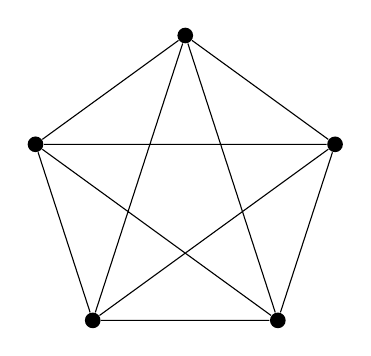
\begin{tikzpicture}
            \node[circle, fill=black, inner sep=2pt] (A) at (90:2) {};
            \node[circle, fill=black, inner sep=2pt] (B) at (162:2) {};
            \node[circle, fill=black, inner sep=2pt] (C) at (234:2) {};
            \node[circle, fill=black, inner sep=2pt] (D) at (306:2) {};
            \node[circle, fill=black, inner sep=2pt] (E) at (18:2) {};
            \draw (A) -- (B) -- (C) -- (D) -- (E) -- (A);
            \draw (A) -- (C) -- (E) -- (B) -- (D) -- (A);
        \end{tikzpicture}
    \end{center}
    Za graf \(K_n\) velja, da je \(\abs{\partial S} = \abs{S} \cdot (n - \abs{S})\). Torej je
    \begin{align*}
        c(K_n) = \min_{S} n-\abs{S}
    \end{align*}
    minimum je dosežen pri \(\abs{S} = \lfloor\frac n2\rfloor\) s poljubno izbiro vozlišč.
    \begin{align*}
        c(K_n) = \left\lceil \frac n2 \right\rceil
    \end{align*}
    Večji kot je \(n\), večja je Cheegerjeva konstanta in graf je bolje povezan.
\end{primer}
Oglejmo si še primer, kjer je zelo očitna povezava med ozkim grlom grafa in Cheegerjevo konstanto.
\begin{primer}[Ozko grlo]\hspace{0em}
    \begin{figure}
        \centering
        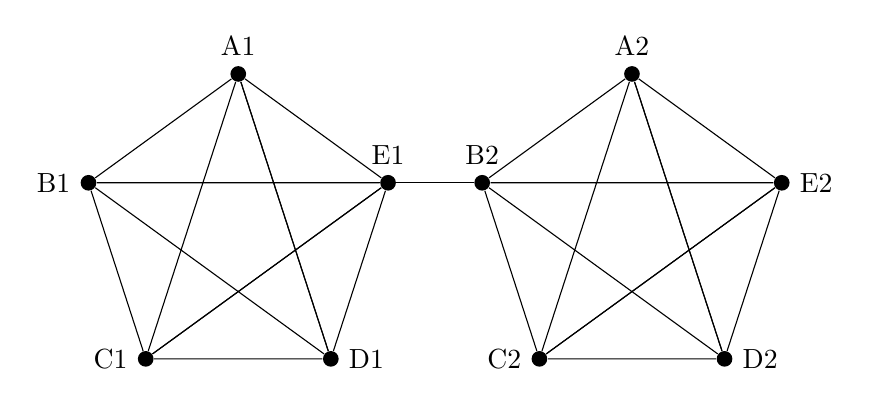
\begin{tikzpicture}
            % First K_5
            \begin{scope}[shift={(0,0)}]
                \node[circle, fill=black, inner sep=2pt, label=above:A1] (A1) at (90:2) {};
                \node[circle, fill=black, inner sep=2pt, label=left:B1] (B1) at (162:2) {};
                \node[circle, fill=black, inner sep=2pt, label=left:C1] (C1) at (234:2) {};
                \node[circle, fill=black, inner sep=2pt, label=right:D1] (D1) at (306:2) {};
                \node[circle, fill=black, inner sep=2pt, label=above:E1] (E1) at (18:2) {};
                \draw (A1) -- (B1) -- (C1) -- (D1) -- (E1) -- (A1);
                \draw (A1) -- (C1) -- (E1) -- (B1) -- (D1) -- (A1);
                \draw (A1) -- (D1);
                \draw (B1) -- (E1);
                \draw (C1) -- (E1);
            \end{scope}

            % Second K_5
            \begin{scope}[shift={(5,0)}]
                \node[circle, fill=black, inner sep=2pt, label=above:A2] (A2) at (90:2) {};
                \node[circle, fill=black, inner sep=2pt, label=above:B2] (B2) at (162:2) {};
                \node[circle, fill=black, inner sep=2pt, label=left:C2] (C2) at (234:2) {};
                \node[circle, fill=black, inner sep=2pt, label=right:D2] (D2) at (306:2) {};
                \node[circle, fill=black, inner sep=2pt, label=right:E2] (E2) at (18:2) {};
                \draw (A2) -- (B2) -- (C2) -- (D2) -- (E2) -- (A2);
                \draw (A2) -- (C2) -- (E2) -- (B2) -- (D2) -- (A2);
                \draw (A2) -- (D2);
                \draw (B2) -- (E2);
                \draw (C2) -- (E2);
            \end{scope}

            % Connecting edge between the two K_5 graphs
            \draw (E1) -- (B2);
        \end{tikzpicture}
        \caption{Povezana grafa \(K_5\)}
    \end{figure}
    Dvem polnim grafom \(K_n\) dodamo povezavo, da dobimo povezan graf \(G = (V,E)\). Če za \(S\) vzamemo enega izmed polnih grafov, je \(\abs{S} = n\) maksimalen in \(\abs{\partial S} = 1\) minimalen. Torej je Cheegerjeva konstanta
    \begin{align*}
        c(G) = \frac{1}{n}.
    \end{align*}
    Večji kot je \(n\), bolj izrazito je ozko grlo na grafu, kar vidimo tudi v manjši \(c(G)\).
\end{primer}
\subsection{Spektralna vrzel}
Graf lahko predstavimo tudi s sosednostno matriko. Vozlišča grafa \(G=(V,E)\) označimo od \(1\) do \(n=\abs{V}\) in naredimo \(n\times n\) matriko \(N(G)\), ki ima vrednost \(1\) na \((i,j)\)-tem mestu, če obstaja povezava med vozliščem \(i\) in \(j\) (oziroma \((i,j)\in E\)). Če povezave ni, je na tistem mestu vrednost \(0\).

Ker so grafi neusmerjeni je matrika simetrična. Po spektralnem izreku ima torej \(n\) realnih lastnih vrednosti \(\lambda_i\), ki jih uredimo po velikosti.
\begin{align*}
    \lambda_1 \geq \lambda_2 \geq \ldots \geq \lambda_n
\end{align*}

\begin{definicija}[Spektralna vrzel]
    Spektralna vrzel grafa \(G\) je razlika med dvema največjima lastnima vrednostima njegove sosednostne matrike.
    \begin{align*}
        s(G) = \lambda_1 - \lambda_2
    \end{align*}
\end{definicija}
\begin{primer}[Cikli]
    Graf \(C_n\) ima sosednostno matriko
    \begin{align*}
        N(C_n) = \begin{bmatrix}
                     0      & 1      & 0      & 0      & \cdots & 0      & 0      & 1      \\
                     1      & 0      & 1      & 0      & \cdots & 0      & 0      & 0      \\
                     0      & 1      & 0      & 1      & \cdots & 0      & 0      & 0      \\
                     \vdots & \vdots & \vdots & \vdots & \ddots & \vdots & \vdots & \vdots \\
                     0      & 0      & 0      & 0      & \cdots & 1      & 0      & 1
                 \end{bmatrix}.
    \end{align*}
    Matrika je cirkulantna, zato poznamo njene lastne vrednosti.
    \begin{align*}
        \lambda(N(C_n)) = \left\{ 2 \cos\left(\frac{2\pi k}{n}\right) \mid 0 \leq k \leq n-1\right\}
    \end{align*}
    % Add source?
    Od tod sledi, da je spektralna vrzel
    \begin{align*}
        s(C_n) = 2 - 2\cos\frac{2\pi}{n}.
    \end{align*}
    Opazimo da večji kot je graf, manjša je spektralna vrzel, prav tako kot je manjša Cheegerjeva konstanta.
\end{primer}
\begin{primer}[Polni grafi]
    Graf \(K_n\) ima sosednostno matriko
    \begin{align*}
        N(K_n) = \begin{bmatrix}
                     0      & 1      & 1      & \cdots & 1      \\
                     1      & 0      & 1      & \cdots & 1      \\
                     1      & 1      & 0      & \cdots & 1      \\
                     \vdots & \vdots & \vdots & \ddots & \vdots \\
                     1      & 1      & 1      & \cdots & 0
                 \end{bmatrix}.
    \end{align*}
    Lastne vrednosti matrike dobimo tako, da uganemo lastne vektorje.
    \begin{align*}
        v_1 = \begin{bmatrix}
                  1      \\
                  1      \\
                  \vdots \\
                  1
              \end{bmatrix} \\
        N(K_n) v_1 = (n-1) \cdot v_1
    \end{align*}
    Torej je ena lastna vrednost \(n-1\). Ostale lastne vektorje \(v_j\) za \(j>1\) dobimo kot
    \begin{align*}
        v_j = e_1 - e_j,
    \end{align*}
    kjer je \(e_j\) enotski vektor z \(1\) v \(j\)-ti komponenti. Ker je
    \begin{align*}
        N(K_n)v_j = -1 \cdot v_j,
    \end{align*}
    dobimo še \(n-1\) lastnih vrednosti \(-1\). Spektralna vrzel je torej
    \begin{align*}
        s(K_n) = (n-1) - (-1) = n.
    \end{align*}
    Opazimo da večji kot je graf, večja je vrzel (prav tako, kot je večja Cheegerjeva konstanta).
\end{primer}
\begin{primer}[Ozko grlo]
    Vzamemo primer dveh grafov \(K_n\), povezanih z eno povezavo. Matrika sosednosti je dimenzije \(2n \times 2n\) in ima na zgornji levi \(n\times n\) podmatriki vrednosti \(1\) povsod razen na diagonali, kjer so vrednosti \(0\). Enako je na spodnji desni \(n\times n\) podmatriki (tako dobimo dva grafa \(K_n\) kot podgrafa). Ostale vrednosti so \(0\), razen na elementu matrike \((1, n+1)\) in \((n+1, 1)\), kjer je vrednost \(1\) (ki predstavlja povezavo med grafoma \(K_n\)).

    Spektralne vrzeli izračunamo numerično in izrišemo na grafu.
    % compute/definicije_spectral_gap_bottleneck.py
    \begin{figure}[h!]
        \centering
        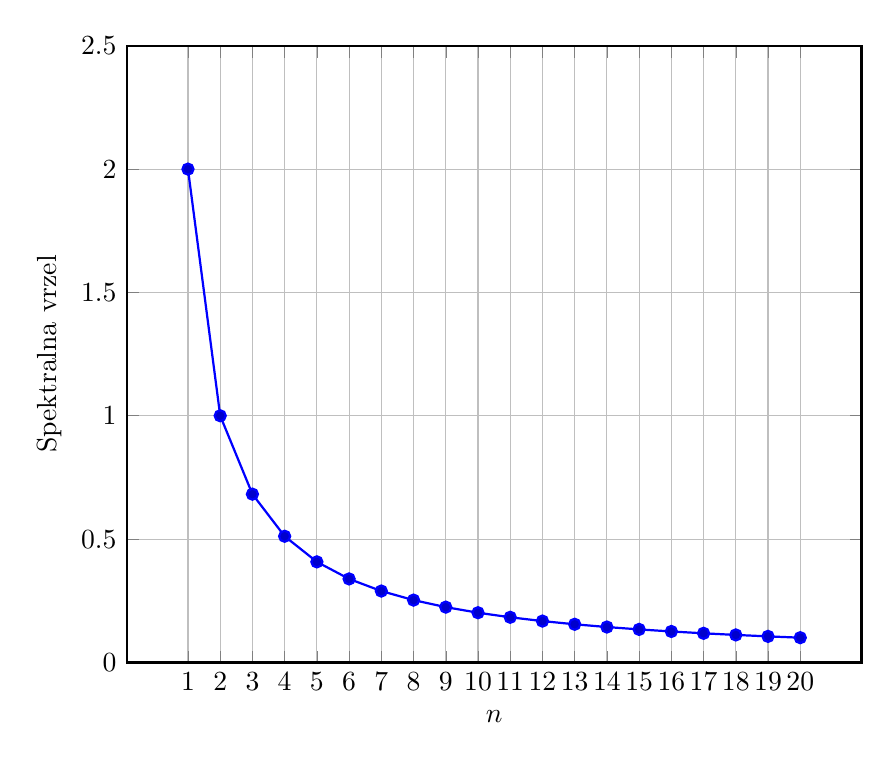
\begin{tikzpicture}
            \begin{axis}[
                    xlabel={$n$},
                    width=0.9\textwidth,
                    ylabel={Spektralna vrzel},
                    grid=major,
                    ymin=0, ymax=2.5,
                    xtick={1,2,...,20},
                    ytick={0,0.5,1,1.5,2,2.5},
                    thick
                ]
                \addplot coordinates {
                        (1, 2.0)
                        (2, 0.9999999999999988)
                        (3, 0.6821627548042195)
                        (4, 0.5114877902540731)
                        (5, 0.40764085275359996)
                        (6, 0.3384804373175667)
                        (7, 0.28929431396096117)
                        (8, 0.2525727509441946)
                        (9, 0.22412614005130305)
                        (10, 0.20144531545046007)
                        (11, 0.18293973049316747)
                        (12, 0.16755365441690628)
                        (13, 0.15455930002271145)
                        (14, 0.14343884532369877)
                        (15, 0.13381387867170424)
                        (16, 0.1254014671437087)
                        (17, 0.11798583829938813)
                        (18, 0.11139957046625426)
                        (19, 0.10551076707121965)
                        (20, 0.10021410708796452)
                    };
            \end{axis}
        \end{tikzpicture}
        \caption{Graf spektralnih vrzeli za \(n\) od 1 do 20}
    \end{figure}
    Opazimo, da večji kot je \(n\), manjša je spektralna vrzel, prav tako kot je manjša Cheegerjeva konstanta (in bolj kot je očitno ozko grlo).
\end{primer}

Računanje lastnih vrednosti regularnega grafa nam olajša tudi lastnost, da je njegova največja lastna vrednost enaka stopnji regularnosti.
\begin{izrek}[Največja vrednost \(d\)-regularnega grafa]
    Največja lastna vrednost \(d\)-regularnega grafa je \(d\).
\end{izrek}
\begin{dokaz}
    Lastni vektor \(d\)-regularnega grafa \(G\) za lastno vrednost \(d\) je vedno vektor samih enic, saj ima vsaka vrstica sosednostne matrike natanko \(n\) enic.

    Večje lastne vrednosti ne obstaja, saj so elementi sosednostne matrike samo \(0\) in \(1\). Če bi obstajala lastna vrednost \(\lambda > d\), potem si ogledamo največji element lastnega vektorja za to lastno vrednost, \(x\). Ker ima matrika natanko \(d\) enic v vsaki vrstici (in ostale vrednosti \(0\)), bi moralo obstajati \(d\) elementov vektorja, ki se skupaj sešteje v \(\lambda x\). Ker pa je vsak element manjši ali enak \(x\), imamo jih pa \(d\) lahko dosežemo kvečjemu \(d \times x\), torej večja lastna vrednost ne obstaja.
\end{dokaz}
Če je graf regularen torej, potrebujemo le izračunati njegovo drugo največjo lastno vrednost.
\subsection{Cheegerjeva neenakost}
Opazili smo, da se Cheegerjeva konstanta in spektralna vrzel obnašata podobno. Definiciji pa nista enakovredni - obstajajo na primer grafi, kjer lahko dodamo povezave ampak znižamo spektralno vrzel (medtem, ko bo Cheegerjeva konstanta ne more postati nižja).

\begin{primer}[Dodajanje povezave poviša vrzel]
    % compute/edges_increase_gap.py
    Kot primer vzamemo graf
    % change the labels to be as in the bottleneck example. Also make h! work
    \begin{figure}[h!]
        \centering
        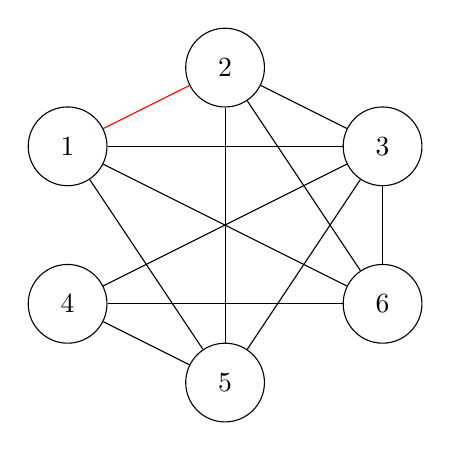
\begin{tikzpicture}[scale=1, every node/.style={circle, draw, minimum size=1cm}]
            % Nodes
            \node (1) at (0,2) {1};
            \node (2) at (2,3) {2};
            \node (3) at (4,2) {3};
            \node (4) at (0,0) {4};
            \node (5) at (2,-1) {5};
            \node (6) at (4,0) {6};

            % Edges based on the adjacency matrix
            \path[draw=red] (1) edge (2);
            \path (1) edge (3);
            \path (1) edge (5);
            \path (1) edge (6);

            \path (2) edge (3);
            \path (2) edge (5);
            \path (2) edge (6);

            \path (3) edge (4);
            \path (3) edge (5);
            \path (3) edge (6);

            \path (4) edge (5);
            \path (4) edge (6);
        \end{tikzpicture}
    \end{figure}
    s sosednostno matriko
    \begin{align*}
        \begin{bmatrix}
            0          & \mathbf{1} & 1 & 0 & 1 & 1 \\
            \mathbf{1} & 0          & 1 & 0 & 1 & 1 \\
            1          & 1          & 0 & 1 & 1 & 1 \\
            0          & 0          & 1 & 0 & 1 & 1 \\
            1          & 1          & 1 & 1 & 0 & 0 \\
            1          & 1          & 1 & 1 & 0 & 0 \\
        \end{bmatrix}.
    \end{align*}
    Spektralna vrzel grafa je približno \(3.706\), če pa odstranimo povezavo med vozliščema \(1\) in \(2\) dobimo spektralno vrzel približno \(3.766\). Tako smo graf naredili slabše povezanega, spektralno vrzel pa vseeno povišali. Cheegerjeva konstanta pa je v obeh primerih enaka \(2\) (kjer za \(S\) lahko vzamemo vozlišča \(1\), \(2\) in \(5\)).
\end{primer}

Kljub temu pa lahko povezavo med konceptoma Cheegerjeve neenakosti in spektralne vrzeli vseeno formaliziramo.
\begin{izrek}[Cheegerjeva neenakost]
    Za \(d\)-regularen graf \(G\) velja 
    \begin{align*}
        \frac{1}{2}s(G) \leq c(G) \leq \sqrt{2ds(G)}
    \end{align*}
    oziroma
    \begin{align*}
        2c(G) \geq s(G) \geq \frac{c(G)^2}{2d}
    \end{align*}    
\end{izrek}
Za dokaz izreka potrebujemo naslednjo lemo.
\begin{lema}\label{cheegerLema}
    Za poljubna \(a, b, c, d > 0\) velja
    \begin{align*}
        \frac{a+b}{c+d} \geq \min\left(\frac{a}{c}, \frac{b}{d}\right).
    \end{align*}
\end{lema}
\begin{dokaz}
    \begin{align*}
        a+b &= c\cdot\frac{a}{c} + d\cdot \frac{a}{d}\\
        a+b &\geq (c+d) \min\left(\frac{a}{c}, \frac{b}{d}\right)\\
        \frac{a+b}{c+d} &\geq \min\left(\frac{a}{c}, \frac{b}{d}\right)
    \end{align*}
\end{dokaz}
\begin{dokaz}[Dokaz Cheegerjeve neenakosti]
    Dokažimo najprej \(2c(G) \geq s(G)\). Naj bo \(S\subset V(G)\) tak, da zadosti minimumu iz definicije Cheegerjeve konstante, torej \(0<\abs{S} \leq \frac12\abs{V(G)}\) in 
    \begin{align*}
        c(G) = \frac{\abs{\partial S}}{\abs{S }}.
    \end{align*}
    Spektralno vrzel poiščemo prek Rayleighovega kvocienta. Če je \(A\) sosednostna matrika grafa je Rayleighov kvocient
    \begin{align*}
        R(A, v) = \frac{v^\top Av}{v^\top v}.
    \end{align*}
    Vemo že, da je vektor samih enic lastni vektor sosednostne matrike za največjo lastno vrednost \(d\). Če torej želimo drugo največjo lastno vrednost, lahko poiščemo maksimum Rayleighovega kvocienta po vseh vektorjih, ki so pravokotni na vektor samih enic. Da pokažemo želeno neenakost izberemo specifičen vektor \(v\) in izračunamo njegov Rayleighov kvocient. Druga največja lastna vrednost bo večja ali enaka od izračunanega kvocienta, spektralna vrzel pa zato manjša.

    Izberemo vektor \(v\) tako, da ima elemente enake \(\frac{1}{\abs{S}}\) na indeksih, ki pripadajo elementom iz \(S\) ter ostale elemente (tiste, ki pripadajo indeksom za \(\overline S\)) enake \(-\frac{1}{\abs{\overline S}}\). Ta vektor je pravokoten na vektor samih enic.
    Sedaj izračunamo Rayleighov kvocient.
    \begin{align*}
        Av = \left(\sum_{j=1}^{\abs{V(G)}} v_j \cdot A_{i,j}\right)_{i=1}^{\abs{V(G)}}\\
        v^\top Av = \sum_{i=1}^{\abs{V(G)}} \sum_{j=1}^{\abs{V(G)}} v_i v_j A_{i,j} = \sum_{i\sim j} v_i v_j\\
    \end{align*}
    \begin{align*}
        R(A, v) &= \frac{\sum_{i\sim j} v_i v_j}{\sum_{i=1}^{\abs{V(G)}}v_i^2}\\
        &= \frac{\sum_{i\sim j} v_i^2 + v_j^2 - \left(v_i - v_j\right)^2}{2 \sum_{i=1}^{\abs{V(G)}}v_i^2}\\
        &= \frac{\sum_{i\sim j} v_i^2}{\sum_{i=1}^{\abs{V(G)}}v_i^2} - \frac{\sum_{i\sim j}\left(v_i - v_j\right)^2}{2 \sum_{i=1}^{\abs{V(G)}}v_i^2}\\
        &= \frac{d\cdot \sum_{i=1}^{\abs{V(G)}}v_i^2}{\sum_{i=1}^{\abs{V(G)}}v_i^2} -  \frac{2\cdot \sum_{i\in S \land j \in \overline S}\left(v_i - v_j\right)^2}{2 \sum_{i=1}^{\abs{V(G)}}v_i^2}\\
        &= d - \frac{\abs{\partial S} \cdot \left(\frac{1}{\abs{S}} + \frac{1}{\abs{\overline S}}\right)^2}{\abs{S} \frac{1}{\abs{S}^2} + \abs{\overline S} \frac{1}{\abs{\overline S}^2}}\\
        &= d - \abs{\partial S}\left(\frac{1}{\abs{S}} + \frac{1}{\abs{\overline S}}\right) \\ 
        &= d - \frac{\abs{\partial S}}{\abs{S}}\frac{\left(\abs{S} + \abs{\overline S}\right)}{\abs{\overline S}}\\
        &= d- c(G) \frac{V(G)}{\abs{\overline S}}\\
        &\geq d - 2c(G)
    \end{align*}
    Torej velja
    \begin{align*}
        \lambda_2 \geq R(A,v) \geq d-2c(G)\\
        2c(G) \geq d-\lambda_2 = s(G)
    \end{align*}

    % file:///home/tadej/library/math/magistrska/cheeger_chung.pdf
    Sedaj dokažemo še drugo neenakost, \(s(G) \geq \frac{c(G)^2}{2d}\). Tu bomo preko Fiedlerjevega algoritma s pomočjo lastnega vektorja za drugo največjo lastno vrednost konstruirali particijo grafa.

    Naj bo \(v\) lastni vektor za drugo največjo lastno vrednost, \(\lambda_2\). Brez škode za splošnost preuredimo vozlišča grafa tako, da je \(v_i \geq v_j\) za \(i < j\). Definiramo \(S_i = \{v_1, \ldots, v_i\}\) in 
    \begin{align*}
        \alpha(G) = \min_{1\leq i \leq V(G)/2} \frac{\abs{\partial S_i}}{\abs{S_i}}.
    \end{align*}
    Očitno je \(h(G) \leq \alpha(G)\).

    Vzamemo \(r=\floor{\frac{V(G)}{2}}\) in definiramo
    \begin{align*}
        v^+_i = \begin{cases}
            v_i - v_r & v_i \geq v_r \\
            0 & v_i < v_r
        \end{cases}\\
        v^-_i = \begin{cases}
            v_r - v_i & v_i \leq v_r \\
            0 & v_i > v_r
        \end{cases}.
    \end{align*}
    Predpostavimo, da velja \(R(A, v^+) \geq R(A, v^-)\), sicer lastni vektor \(v\) pomnožimo z \(-1\). Izbrali smo \(r\) tako, da bosta vedno oba vektorja (\(v^+\) in \(v^-\)) imela kvečjemu \(r\) pozitivnih elementov, kar se ohrani, če zamenjamo predznake v vektorju \(v\), kot zahteva predpostavka. Vozlišča, ki pripadajo pozitivnim elementom \(v^+\) bomo uporabili pri vpeljavi \(\alpha(G)\), ki pa zahteva podgraf velikosti največ \(r\). Predpostavko lahko zapišemo tudi drugače:
    \begin{align}\label{eq:cheegerPredpostavka}
        \frac{\sum_{i\sim j}(v^+_i - v^+_j)^2}{2\sum_{i=1}^{\abs{V(G)}} (v^+_i)^2} \leq \frac{\sum_{i\sim j} (v^-_i - v^-_j)^2}{2\sum_{i=1}^{\abs{V(G)}} (v^-_i)^2} 
    \end{align}

    Podobno kot v prvem delu dokaza preko Rayleighovega kvocienta izrazimo spektralno luknjo.
    \begin{align*}
        s(G) &= d-\lambda_2 \\ 
        &= \frac{\sum_{i\sim j}(v_i - v_j)^2}{2\sum_{i=1}^{\abs{V(G)}} v_i^2}
    \end{align*}
    
    Ker je \(v\) pravokoten na največji lastni vektor, vektor samih enic, velja \(\sum_i v_i = 0\). Tako lahko povečamo imenovalec kvocienta:
    \begin{align*}
        \sum_{i=1}^{\abs{V(G)}} v_i^2 = \min_{c\in \R} \sum_{i=1}^{\abs{V(G)}} (v_i - c)^2 \leq \sum_{i=1}^{\abs{V(G)}} (v_i - v_r)^2\\
        \frac{\sum_{i\sim j}(v_i - v_j)^2}{2\sum_{i=1}^{\abs{V(G)}} v_i^2} \geq \frac{\sum_{i\sim j}(v_i - v_j)^2}{2\sum_{i=1}^{\abs{V(G)}} (v_i-v_r)^2}
    \end{align*}
    Imenovalec lahko prepišemo z uporabo \(v^+\) in \(v^-\)
    \begin{align*}
        \frac{\sum_{i\sim j}(v_i - v_j)^2}{2\sum_{i=1}^{\abs{V(G)}} v_i^2} \geq \frac{\sum_{i\sim j}(v_i - v_j)^2}{2\sum_{i=1}^{\abs{V(G)}} (v_i-v_r)^2} = \frac{\sum_{i\sim j}(v_i - v_j)^2}{2\sum_{i=1}^{\abs{V(G)}} (v^+_i)^2 + 2\sum_{i=1}^{\abs{V(G)}} (v^-_i)^2}.
    \end{align*}
    
    Sedaj pomanjšamo števec \(\sum_{i\sim j}(v_i - v_j)^2\). Če sta \(v_i\) in \(v_j\) oba večja od \(v_r\), potem velja
    \begin{align*}
        (v_i - v_j)^2 = (v^+_i - v^+_j)^2 + (v^-_i - v^-_j)^2.
    \end{align*}
    Enako velja, če sta oba manjša od \(v_r\). V primeru ko je \(v_j \leq v_r \leq v_i\), pa vidimo slednje:
    \begin{align*}
        0 \geq (v_r - v_i)(v_r - v_j)\\
        0 \geq v_r^2 - v_r v_i - v_r v_j + v_i v_j \\
        -2 v_i v_j \geq 2 v_r^2 - 2 v_r v_i - 2 v_r v_j \\
        v_i^2 - 2v_i v_j + v_j^2 \geq (v_r^2 - 2v_r v_i + v_i^2) + (v_r^2 - 2v_r v_j + v_j^2) \\ 
        (v_i - v_j)^2 \geq (v_i - v_r -0)^2 + (0 + v_j - v_r)^2 \\
        (v_i - v_j)^2 \geq  (v^+_i - v^+_j)^2 + (v^-_i - v^-_j)^2
    \end{align*}
    Enako velja v primeru \(v_i \leq v_r \leq v_j\), torej je
    \begin{align*}
        s(G) &\geq \frac{\sum_{i\sim j}(v_i - v_j)^2}{2\sum_{i=1}^{\abs{V(G)}} (v^+_i)^2 + 2\sum_{i=1}^{\abs{V(G)}} (v^-_i)^2}\\
        &\geq \frac{\sum_{i\sim j}(v^+_i - v^+_j)^2 + (v^-_i - v^-_j)^2}{2\sum_{i=1}^{\abs{V(G)}} (v^+_i)^2 + 2\sum_{i=1}^{\abs{V(G)}} (v^-_i)^2}
    \end{align*}
    
    Zgornjo neenakost lahko, s pomočjo predpostavke \eqref{eq:cheegerPredpostavka} in leme \ref{cheegerLema} spremenimo v

    \begin{align*}
        s(G) \geq  \frac{\sum_{i\sim j}(v^+_i - v^+_j)^2}{2\sum_{i=1}^{\abs{V(G)}} (v^+_i)^2}.
    \end{align*}
    Od tod sledi
    \begin{align*}
        s(G) &\geq  \frac{\sum_{i\sim j}(v^+_i - v^+_j)^2}{2\sum_{i=1}^{\abs{V(G)}} (v^+_i)^2} \frac{\sum_{i\sim j}(v^+_i + v^+_j)^2}{\sum_{i\sim j}(v^+_i + v^+_j)^2}\\
        &= \frac{\sum_{i\sim j}(v^+_i - v^+_j)^2}{2\sum_{i=1}^{\abs{V(G)}} (v^+_i)^2} \frac{\sum_{i\sim j}(v^+_i + v^+_j)^2}{\sum_{i\sim j}(v^+_i)^2 + (v^+_j)^2 + 2v^+_i v^+_j}\\
        &= \frac{\sum_{i\sim j}(v^+_i - v^+_j)^2}{2\sum_{i=1}^{\abs{V(G)}} (v^+_i)^2} \frac{\sum_{i\sim j}(v^+_i + v^+_j)^2}{2d\sum_{i=1}^{\abs{V(G)}} (v^+_i)^2 + 2\sum_{i\sim j}v^+_i v^+_j}
    \end{align*}
    Uporabimo Cauchy-Schwarzovo neenakost ločeno na števcu in na delu imenovalca.
    \begin{align*}
        s(G) &\geq  \frac{\left(\sum_{i\sim j}(v^+_i - v^+_j)(v^+_i + v^+_j)\right)^2}{2\sum_{i=1}^{\abs{V(G)}} (v^+_i)^2\left(2d\sum_{i=1}^{\abs{V(G)}} (v^+_i)^2 + 2\sqrt{\sum_{i\sim j}(v^+_i)^2 \sum_{i\sim j} (v^+_j)^2}\right)}\\
        &= \frac{\left(\sum_{i\sim j}\abs{(v^+_i)^2 - (v^+_j)^2} \right)^2}{2\sum_{i=1}^{\abs{V(G)}} (v^+_i)^2 \left(2d\sum_{i=1}^{\abs{V(G)}} (v^+_i)^2 + 2d \sum_{i=1}^{\abs{V(G)}}(v^+_i)^2 \right)}\\
        &= \frac{\left(\sum_{i\sim j}\abs{(v^+_i)^2 - (v^+_j)^2} \right)^2}{8d\left(\sum_{i=1}^{\abs{V(G)}} (v^+_i)^2\right)^2}\\
        &= \frac{\left(2\sum_{i\sim j \land i< j}(v^+_i)^2 - (v^+_j)^2 \right)^2}{8d\left(\sum_{i=1}^{\abs{V(G)}} (v^+_i)^2\right)^2} \\
        &= \frac{\left(\sum_{i\sim j \land i< j}(v^+_i)^2 - (v^+_j)^2 \right)^2}{2d\left(\sum_{i=1}^{\abs{V(G)}} (v^+_i)^2\right)^2}
    \end{align*}
    Vsak sumand \((v^+_i)^2 - (v^+_j)^2\) lahko teleskopsko razpišemo kot
    \begin{align*}
        (v^+_i)^2 &- (v^+_{i+1})^2\\
        + (v^+_{i+1})^2 &- (v^+_{i+2})^2\\
        + &\cdots\\
        + (v^+_{j-1})^2 &- (v^+_{j})^2,
    \end{align*}
    da dobimo
    \begin{align*}
        s(G) &\geq \frac{\left(\sum_{i=1}^{\abs{V(G)}}\abs{\partial S_i}\left((v^+_i)^2 - (v^+_{i+1})^2\right) \right)^2}{2d\left(\sum_{i=1}^{\abs{V(G)}} (v^+_i)^2\right)^2}
        &=\frac{\left(\sum_{i=1}^{r}\abs{\partial S_i}\left((v^+_i)^2 - (v^+_{i+1})^2\right) \right)^2}{2d\left(\sum_{i=1}^{r} (v^+_i)^2\right)^2}
    \end{align*}
    Po definiciji za vsak \(i\leq r\) velja \(\abs{\partial S_i} \geq \abs{S_i} \alpha(G)\).
    \begin{align*}
        s(G) &\geq \frac{\left(\sum_{i=1}^{r} \abs{S_i} \alpha(G)\left((v^+_i)^2 - (v^+_{i+1})^2\right) \right)^2}{2d\left(\sum_{i=1}^{r} (v^+_i)^2\right)^2}\\
        &= \frac{\alpha(G)^2}{2d} \frac{\left(\sum_{i=1}^{r} \abs{S_i}\left((v^+_i)^2 - (v^+_{i+1})^2\right) \right)^2}{\left(\sum_{i=1}^{r} (v^+_i)^2\right)^2}\\
        &= \frac{\alpha(G)^2}{2d} \frac{\left(\sum_{i=1}^{r} i\cdot (v^+_i)^2 - \sum_{i=1}^{r} (i-1) \cdot (v^+_{i})^2 \right)^2}{\left(\sum_{i=1}^{r} (v^+_i)^2\right)^2}\\
        &= \frac{\alpha(G)^2}{2d} \frac{\left(\sum_{i=1}^{r} i\cdot (v^+_i)^2 - \sum_{i=1}^{r} (i-1) \cdot (v^+_{i})^2 \right)^2}{\left(\sum_{i=1}^{r} (v^+_i)^2\right)^2}\\
        &= \frac{\alpha(G)^2}{2d} \frac{\left(\sum_{i=1}^{r} \cdot (v^+_i)^2 \right)^2}{\left(\sum_{i=1}^{r} (v^+_i)^2\right)^2}\\
        &= \frac{\alpha(G)^2}{2d}\\
    \end{align*}
    Tako dobimo
    \begin{align*}
        s(G) \geq \frac{\alpha(G)^2}{2d} \geq \frac{h(G)^2}{2d}
    \end{align*}



\end{dokaz}
\subsection{Alon-Boppanov izrek}
\subsection{Ramanujanovi grafi}
\section{Naključne konstrukcije}
Cilj poglavja je generiranje Ramanujanovih grafov na računalniku. Uporabili bomo najenostavnejši algoritem: generiramo naključen \(d\)-regularen graf in izračunamo njegovo spektralno vrzel. Če je dovolj velika, je naš graf Ramanujanov, če pa je premajhna, graf zavržemo in generiramo nov graf, dokler ne dobimo takega, ki ima dovolj veliko spektralno vrzel. Računanje lastnih vrednosti grafa je zelo enostavno, zato si bomo podrobneje ogledali le algoritem za učinkovito generiranje naključnih regularnih grafov.

S pomočjo dobljenega algoritma si lahko ogledamo nekaj lastnosti grafov. Zanima nas velikost spektralne vrzeli v odvisnosti od števila vozlišč in delež Ramanujanov grafov. Če je ta delež dovolj velik, je naš algoritem učinkovit in lahko enostavno generiramo Ramanujanove grafe. Velikost povprečne spektralne vrzeli pa nam pove, kako daleč je poljuben graf od tega, da je Ramanujanov; Ramanujanovi grafi imajo sicer zanimive matematične lastnosti, v praksi bi se pa morda kdaj zadovoljili že z grafom, ki je ``približno'' Ramanujanov.

\subsection{Algoritmi za generiranje regularnih grafov}
Generiranje regularnih grafov je netrivialen problem. Težava pri večini pristopov je, da ne moremo povezav dodajati iterativno in imeti zagotovljeno, da na koncu dobimo regularen graf. Oglejmo si to na enostavnem primeru.

\begin{primer}
    Za primer bomo poskusili generirati \(2\)-regularen graf na štirih vozliščih. Tak graf seveda obstaja, na primer cikel \(C_4\). Naš algoritem bo sledeč: izberemo naključni dve vozlišči, ki imata stopnjo manjšo od \(2\) in ju povežemo. To ponavljamo, dokler ne dobimo grafa, ki je \(2\)-regularen.

    Začnemo s praznim grafom, ki ima vozlišča \(\{1, 2, 3, 4\}\). Izberemo naključni dve vozlišči, recimo \(1\) in \(2\), in ju povežemo. Nato izberemo vozlišči \(2\) in \(3\) in ju povežemo, zatem pa še \(3\) in \(1\) in ju povežemo. Sedaj imamo \(3\) vozlišča stopnje \(2\) in enega stopnje \(0\). Ob vsaki točki smo izbrali vozlišči, ki imata stopnjo manjšo od \(2\), algoritem pa se ne more zaključiti, saj smo prišli do točke, ko vozlišča \(4\) ne moremo povezati z nobenim vozliščem, ki ima stopnjo manjšo od \(2\).
\end{primer}

V tem primeru je bil problem, da ne moremo povezati vozlišča s samim seboj, lahko pa bi se zgodilo tudi, da imamo dve vozlišči stopnje \(d-1\), ki pa ju ne moremo povezati, saj sta že povezani. Obstaja enostaven način, kako lahko rešimo to težavo: če algoritma ne moremo zaključiti, graf zavržemo in začnemo znova. Z malo optimizacije nas to prinese do algoritma \ref{enakomerno-nakljucni-pocasi}, ki generira kandidate, in algoritma \ref{enakomerno-nakljucni-pomozno}, ki ponavlja klice na algoritem \ref{enakomerno-nakljucni-pocasi}, dokler ne dobimo veljavnega regularnega grafa \cite{kim-vu-regularni}. Algoritem \ref{enakomerno-nakljucni-pomozno} bomo uporabljali tudi pri vseh ostalih pristopih za generiranje regularnih grafov.

\algnewcommand\algorithmicto{\textbf{to}}
\algnewcommand\algorithmicin{\textbf{in}}
\algnewcommand\algorithmicforeach{\textbf{for each}}
\algrenewtext{For}[3]{\algorithmicfor\ #1 $\gets$ #2\ \algorithmicto\ #3\ \algorithmicdo}
\algdef{S}[FOR]{ForEach}[2]{\algorithmicforeach\ #1\ \algorithmicin\ #2\ \algorithmicdo}

\begin{algorithm}[t]
    \caption{Generiranje naključnih regularnih grafov}
    \label{enakomerno-nakljucni-pomozno}
    \raggedright
    \textbf{Vhod:} Števili \(n, d \in \mathbb N\). \\
    \textbf{Izhod:} Sosednostna matrika \(A\) \(d\)-regularnega grafa na \(n\) vozliščih.
    \begin{algorithmic}[1]
        \Function{generiraj}{$n$, $d$}
        \While{True}
        \State \(A \gets \Call{generiraj-pomozno}{n, d}\)
        \If{\Call{je-regularen-graf}{$A$, $d$}}
        \State \Return $A$
        \EndIf
        \EndWhile
        \EndFunction
    \end{algorithmic}
\end{algorithm}

\begin{algorithm}[t]
    \caption{Generiranje naključnih regularnih grafov}
    \label{enakomerno-nakljucni-pocasi}
    \raggedright
    \textbf{Vhod:} Števili \(n, d \in n, d \in \mathbb N\). \\
    \textbf{Izhod:} Sosednostna matrika \(A\) \(d\)-regularnega grafa na \(n\) vozliščih.
    \begin{algorithmic}[1]
        \Function{generiraj-pomozno}{$n$, $d$}
        \For{$i$}{$0$}{$n-1$}
        \For{$j$}{$0$}{$d-1$}
        \State \(krajisce[i\cdot n + j] \gets i\) \Comment{Ustvarimo \(d\) kopij vsakega vozlišča.}
        \EndFor
        \EndFor
        \State \(krajisce' \gets \Call{shuffle}{krajisce}\)
        \State \(A \gets\) ničelna matrika velikosti \(n \times n\)
        \For{$i$}{$0$}{$n\cdot d - 1$}
        \State \(A_{krajisce[i], krajisce'[i]} \gets 1\)
        \State \(A_{krajisce'[i], krajisce[i]} \gets 1\)
        \EndFor
        \State \Return $A$
        \EndFunction
    \end{algorithmic}
\end{algorithm}

Algoritem \ref{enakomerno-nakljucni-pocasi} je sicer pravilen, vendar pa je zelo počasen. Velikokrat se zgodi, da moramo ponovno generirati graf, še posebej za velike \(d\), zaradi česar postane neuporaben za generiranje večjih grafov. Izkaže se, da je verjetnost generiranja regularnega grafa \(O(e^{-\frac{d^2}{4}})\) \cite{STEGER_WORMALD_1999}, kar se zelo hitro približuje \(0\), ko povečujemo \(d\). Algoritem postane nepraktičen že, če želimo generirati \(10\)-regularne grafe. Obstajajo algoritmi s polinomsko časovno zahtevnostjo, vendar so še vedno počasni in njihova implementacija je zahtevna. Delo si lahko olajšamo tako, da grafov ne generiramo enakomerno naključno \cite{STEGER_WORMALD_1999}.

Algoritem za hitro generiranje naključnih grafov vsakemu vozlišču priredi \(d\) števil. Najpreprosteje je, da vozlišču \(i\) priredimo števila od \(i\) do vključno \(i+d-1\). Algoritem uporablja še pomožno funkcijo, ki preveri, če je par vozlišč ustrezen za to, da med vozliščema dodamo novo povezavo. Ta funkcija sprejme dve števili, ki sta prirejeni vozliščema in vrne, da par ni ustrezen, če sta dani vozlišči enaki ali pa sta že povezani. Nato enakomerno naključno med vsemi doslej neizbranimi števili izbiramo veljavne pare števil, prirejenih vozliščem, dokler je to mogoče. Ker smo vsakemu vozlišču priredili le \(d\) števil, je torej lahko izbranih kvečjemu \(d\) parov, ki vsebujejo število, ki pripada izbranemu vozlišču. Ko dobimo veljaven par, izračunamo, katerim vozliščem pripadajo prirejena števila ter ta vozlišča povežemo. Glavna pohitritev algoritma prihaja iz dejstva, da je večja verjetnost, da izberemo vozlišče, ki še nima veliko povezav, saj izbiramo enakomerno naključno med neizbranimi prirejenimi števili, vsako izbrano število pa predstavlja obstoječo povezavo.

\begin{algorithm}[t]
    \caption{Hitro generiranje naključnih regularnih grafov}
    \label{enakomerno-nakljucni-hitro}
    \raggedright
    \textbf{Vhod:} Števili \(n, d \in \mathbb N\). \\
    \textbf{Izhod:} Sosednostna matrika \(A\) \(d\)-regularnega grafa na \(n\) vozliščih.
    \begin{algorithmic}[1]
        \Function{ustrezen-par}{$i$, $j$, $pari$, $V$}
        \State \(i'\) tak, da \(i\in V[i']\)
        \State \(j'\) tak, da \(j\in V[j']\)
        \If{\(i' = j'\)}
        \State \Return False \Comment{Povezati želimo vozlišče s seboj.}
        \EndIf
        \If{\((i', j') \in pari\)}
        \State \Return False \Comment{Povezava že obstaja.}
        \EndIf
        \State \Return True
        \EndFunction
        \Function{generiraj-pomozno}{$n$, $d$}
        \State \(U = \{1, 2, \ldots, nd\}\) \Comment{Točke, ki še nimajo para.}
        \For {$i$}{$0$}{$n-1$}
        \For {$j$}{$0$}{$d-1$}
        \State \(V[i][j] \gets i\cdot n + j\) \Comment{Ustvarimo \(d\) elementov za vsako vozlišče.}
        \EndFor
        \EndFor
        \State \(pari \gets []\)
        \While{\(\exists i,j \in U.\, \Call{ustrezen-par}{i, j, pari, V}\)}
        \State \(i\gets \Call{nakljucno-izberi}{U}\)
        \State \(j\gets \Call{nakljucno-izberi}{U}\)
        \If {\(\Call{ustrezen-par}{i, j, pari, V}\)}
        \State Dodaj par \((i, j)\) v \(pari\)
        \State Izbriši \(i\) in \(j\) iz \(U\)
        \EndIf
        \EndWhile
        \State \(A \gets\) ničelna matrika velikosti \(n \times n\)
        \ForEach{$(i, j)$}{$pari$}
        \State{\(i'\) tak, da \(i\in V[i']\)}
        \State{\(j'\) tak, da \(j\in V[j']\)}
        \State \(A_{i', j'} \gets 1\)
        \State \(A_{j', i'} \gets 1\)
        \EndFor
        \State \Return $A$
        \EndFunction
    \end{algorithmic}
\end{algorithm}

Za naše potrebe je algoritem \ref{enakomerno-nakljucni-hitro} zadovoljivo hiter in ga bomo uporabljali v nadaljevanju. Algoritem je tudi implementiran v Pythonovi knjižnici za delo z grafi, NetworkX \cite{networkx}. Čeprav grafov ne generira enakomerno naključno, se porazdelitev dobljenih grafov približuje enakomerni, ko večamo število vozlišč. Z algoritmom lahko na običajnih osebnih računalnikih generiramo grafe z do \(10^5\) vozlišči v nekaj sekundah.

Omenimo še preprostejši algoritem \ref{naivno-generiranje-nakljucnih}, ki predstavlja naiven pristop za generiranje regularnih grafov. Tu je implementacija zelo enostavna in program deluje razmeroma hitro, vendar njegova porazdelitev ni niti približno enakomerna. Algoritem iterira po vsakem vozlišču. V dani iteraciji izračuna stopnjo \(d'\) ter poišče \(d-d'\) vozlišč, ki imajo stopnjo nižjo od \(d\) in še niso povezana s trenutnim vozliščem. Če toliko ustreznih vozlišč ni, grafa ne moremo dobiti in bomo morali postopek ponoviti od začetka, sicer pa jih povežemo in nadaljujemo z naslednjim vozliščem. 

\begin{algorithm}[t]
    \caption{Enostavno generiranje naključnih regularnih grafov}
    \label{naivno-generiranje-nakljucnih}
    \raggedright
    \textbf{Vhod:} Števili \(n, d \in \mathbb N\). \\
    \textbf{Izhod:} Sosednostna matrika \(A\) \(d\)-regularnega grafa na \(n\) vozliščih.
    \begin{algorithmic}[1]
        \Function{generiraj-pomozno}{$n$, $d$}
        \State \(A \gets\) ničelna matrika velikosti \(n \times n\)
        \For {$i$}{$0$}{$n-1$}
        \State \(V \gets \) množica vozlišč, stopnje manj od \(d\), ki niso povezana z \(i\)
        \State \(d' \gets \Call{Stopnja}i\)
        \If {\(\abs{V} < d-d'\)}
        \State \Return \(A\)
        \EndIf
        \State \(V' \gets \) naključnih \(d-d'\) vozlišč iz \(V\)
        \State Dodamo povezave med \(i\) in vozlišči iz \(V'\) v \(A\)
        \EndFor
        \State \Return $A$
        \EndFunction
    \end{algorithmic}
\end{algorithm}

\subsection{Statistika}
Zdaj imamo učinkovit način generiranja regularnih grafov, torej si lahko ogledamo nekaj lastnosti, povezane z Ramanujanovimi grafi. Ogledali si bomo povprečno velikost največje netrivialne lastne vrednosti grafov ter delež grafov, ki so Ramanujanovi. To bomo pogojevali na število vozlišč in stopnjo regularnosti grafa. Zaključili pa bomo še z analizo porazdelitve lastnih vrednosti in s sliko, ki nam prikaže pomembnost meje \(2\sqrt{d-1}\).

\subsubsection{Lastne vrednosti}
Za začetek si oglejmo, kako se spreminja \(\lambda(G)\) glede na število vozlišč in stopnjo regularnosti grafa \(G\). Uporabljali bomo algoritem \ref{enakomerno-nakljucni-hitro} za hitro generiranje regularnih grafov. Nato bomo za vsako izbrano število vozlišč in stopnjo regularnosti generirali 1000 grafov \(G\) ter izračunali povprečje njihovih \(\lambda(G)\). Ogledali si bomo tri različne stopnje regularnosti: \(d=5\), \(d=11\) in \(d=21\).

Najprej si oglejmo graf za \(d=5\). Tukaj je meja za Ramanujanove grafe \(2\sqrt{5-1} = 4\). Začnemo pri grafu s šestimi vozlišči in izračunamo povprečje \(\lambda(G)\). Nato povečamo število vozlišč za \(20\) in ponovimo postopek. To ponavljamo, dokler imajo grafi manj kot \(600\) vozlišč. Rezultate prikažemo na grafu, dodamo pa še horizontalno črto pri vrednosti \(4\).

\begin{figure}[t]
    \centering
    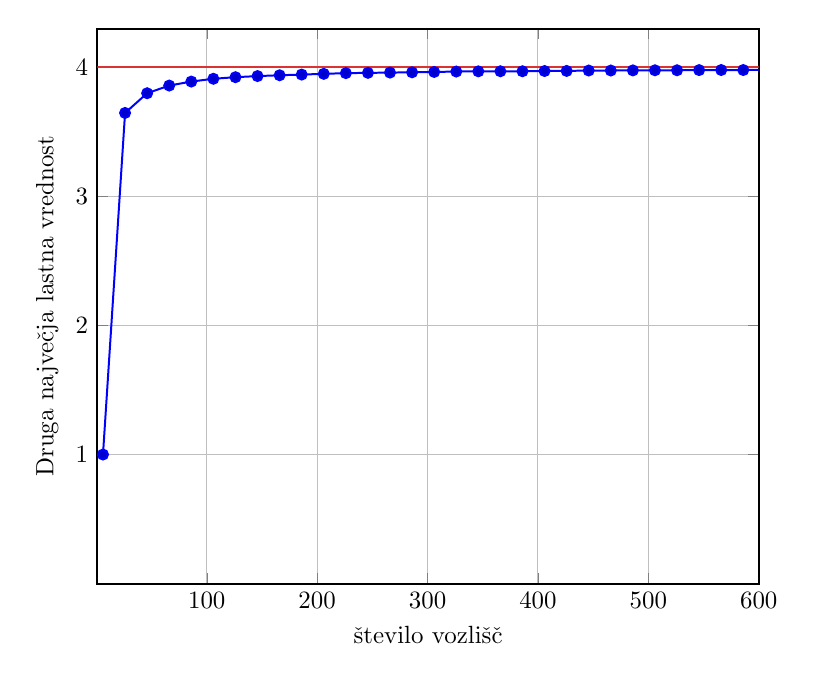
\begin{tikzpicture}[scale=0.9]
        \definecolor{pleasantred}{rgb}{0.85, 0.2, 0.2}
        \begin{axis}[
            xlabel={število vozlišč},
            width=0.9\textwidth,
            ylabel={Druga največja lastna vrednost},
            grid=major,
            ymin=0, ymax=4.3,
            xmin=1, xmax=600,
            xtick={0,100,...,600},
            ytick={1,2,3,4},
            thick
            ]
            \draw[draw=pleasantred] (axis cs:0,4) -- (axis cs:600,4);
            \addplot coordinates {
                (6, 1.0000000000000002)
                (26, 3.6469425449844923)
                (46, 3.79963239469457)
                (66, 3.8590979945057677)
                (86, 3.8900142704961667)
                (106, 3.9116565426594128)
                (126, 3.9238905598334965)
                (146, 3.9325600246589594)
                (166, 3.938855777384826)
                (186, 3.944147515902753)
                (206, 3.9498671033019517)
                (226, 3.9552616354117065)
                (246, 3.957467810537496)
                (266, 3.959490001307144)
                (286, 3.9618796798493063)
                (306, 3.9644616694659205)
                (326, 3.9676602186376644)
                (346, 3.9692542741810946)
                (366, 3.9698360851495904)
                (386, 3.9698257500021206)
                (406, 3.97181111813395)
                (426, 3.972473010011027)
                (446, 3.975603794486935)
                (466, 3.9756303352387716)
                (486, 3.9766439267420317)
                (506, 3.977488063510781)
                (526, 3.9776682760947293)
                (546, 3.978964750149576)
                (566, 3.979531750065059)
                (586, 3.9794685667065974)
                (606, 3.9811456508027763)
                };
            \end{axis}
        \end{tikzpicture}
        \caption{Graf povprečij \(\lambda(G)\) \(5\)-regularnih grafov v odvisnosti od števila vozlišč}
        \label{fig:5-regular}
\end{figure}

Na sliki \ref{fig:5-regular} vidimo, da se povprečje lastnih vrednosti približuje ravno meji za Ramanujanove grafe! Postopek ponovimo še za grafe s stopnjama \(d=11\) in \(d=21\) in tudi v teh primerih opazimo približevanje Ramanujanovi meji.
\begin{figure}[t]
    \centering
    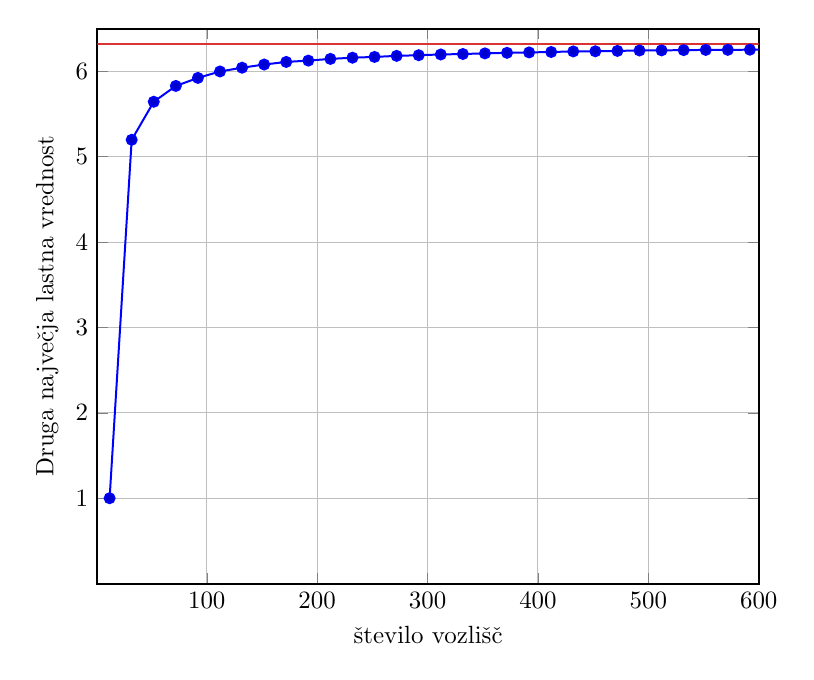
\begin{tikzpicture}[scale=0.9]
        \definecolor{pleasantred}{rgb}{0.85, 0.2, 0.2}
        \begin{axis}[
            xlabel={število vozlišč},
            width=0.9\textwidth,
            ylabel={Druga največja lastna vrednost},
                grid=major,
                ymin=0, ymax=6.5,
                xmin=1, xmax=600,
                xtick={0,100,...,600},
                ytick={1,2,3,4,5,6},
                thick
            ]
            \draw[draw=pleasantred] (axis cs:0,6.324555320336759) -- (axis cs:600,6.324555320336759);
            \addplot coordinates {
                (12, 1.0000000000000002)
                (32, 5.198156377614785)
                (52, 5.643885284747165)
                (72, 5.829117444893516)
                (92, 5.923172524513979)
                (112, 5.998622178810724)
                (132, 6.042619064245882)
                (152, 6.079957685856226)
                (172, 6.11026242602795)
                (192, 6.125752222542846)
                (212, 6.14580019144193)
                (232, 6.159810079904397)
                (252, 6.168875088596623)
                (272, 6.18128569012168)
                (292, 6.189017996514279)
                (312, 6.197667854719561)
                (332, 6.203055775141022)
                (352, 6.210376446059419)
                (372, 6.2170465023897865)
                (392, 6.221533675435159)
                (412, 6.226668634957975)
                (432, 6.23348367206533)
                (452, 6.234805834700305)
                (472, 6.23927709112199)
                (492, 6.244446713350618)
                (512, 6.24568687387802)
                (532, 6.248511105653832)
                (552, 6.25088144542781)
                (572, 6.251713414323658)
                (592, 6.253516933929778)
                (612, 6.254946081316828)
                };
        \end{axis}
    \end{tikzpicture}
    \caption{Graf povprečij \(\lambda(G)\) \(11\)-regularnih grafov v odvisnosti od števila vozlišč}
    \label{fig:11-regular}
\end{figure}

\begin{figure}[t]
    \centering
    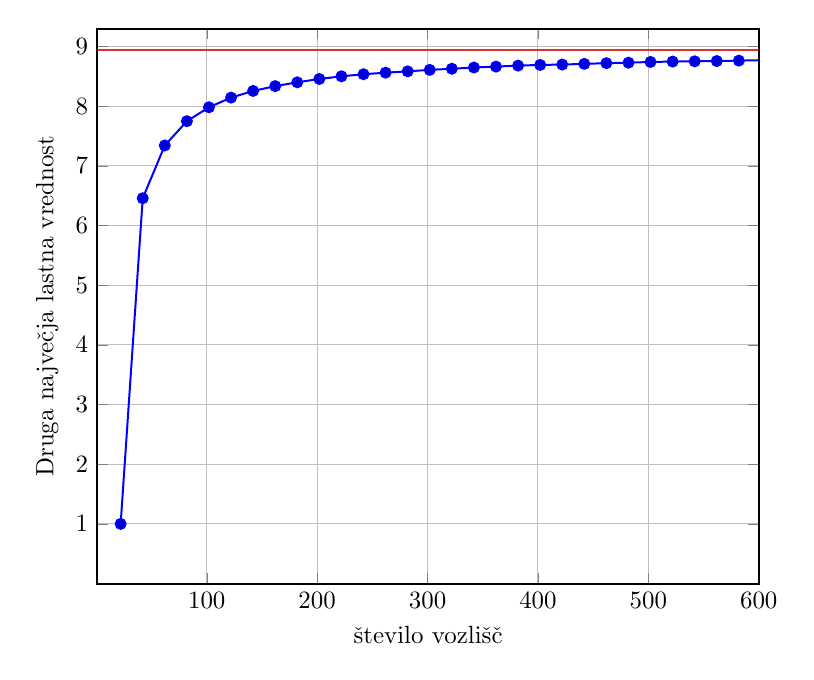
\begin{tikzpicture}[scale=0.9]
        \definecolor{pleasantred}{rgb}{0.85, 0.2, 0.2}
        \begin{axis}[
            xlabel={število vozlišč},
            width=0.9\textwidth,
            ylabel={Druga največja lastna vrednost},
            grid=major,
            ymin=0, ymax=9.3,
            xmin=1, xmax=600,
            xtick={0,100,...,600},
            ytick={1,2,3,4,5,6,7,8,9},
            thick
            ]
            \draw[draw=pleasantred] (axis cs:0,8.94427190999916) -- (axis cs:600,8.94427190999916);
            \addplot coordinates {
                (22, 1.0000000000000016)
                (42, 6.457762460689075)
                (62, 7.34267381875069)
                (82, 7.749182706134452)
                (102, 7.9826028554188175)
                (122, 8.144251955483162)
                (142, 8.256172883115111)
                (162, 8.33681314660636)
                (182, 8.400759701073772)
                (202, 8.456929688398343)
                (222, 8.50117677868208)
                (242, 8.536147098061887)
                (262, 8.562439059545776)
                (282, 8.584384770184979)
                (302, 8.609496150772358)
                (322, 8.627941976386401)
                (342, 8.649075592875864)
                (362, 8.664258721715953)
                (382, 8.680621349648668)
                (402, 8.691973426726586)
                (422, 8.69812122565171)
                (442, 8.709986877027816)
                (462, 8.72164670988282)
                (482, 8.729634460708713)
                (502, 8.741916828498463)
                (522, 8.748384221744477)
                (542, 8.75275208966012)
                (562, 8.757330480876565)
                (582, 8.764164575308484)
                (602, 8.771656193932213)
                };
            \end{axis}
        \end{tikzpicture}
        \caption{Graf povprečij \(\lambda(G)\) \(21\)-regularnih grafov v odvisnosti od števila vozlišč}
        \label{fig:21-regular}
    \end{figure}

\subsection{Delež Ramanujanovih grafov}
Nadaljujemo z deležom Ramanujanovih grafov. Postopek bo enak kot prej, le da rišemo vse hkrati na enem grafu. Da dobimo boljše rezultate si tokrat ogledamo tudi grafe z več vozlišči. Začnemo z grafi, ki imajo manj kot \(1000\) vozlišč, za tem pa tudi izračunamo delež Ramanujanovih grafov za grafe z do \(10^5\) vozlišči. Zaradi časovne zahtevnosti za tako velike grafe izračunamo delež v korakih po \(10 000\) vozlišč. Pri tako velikih grafih je za sosednostne matrike potrebno uporabljati razpršene matrike, da prostorska zahtevnost raste linearno in ne kvadratično. Brez razpršenih matrik bi v primeru \(n=10^5\) in \(d=21\) program porabil okoli \(40\) GB pomnilnika, če pa uporabimo razpršene matrike pa le okoli \(10\) MB.

\begin{figure}[t]
    \centering
    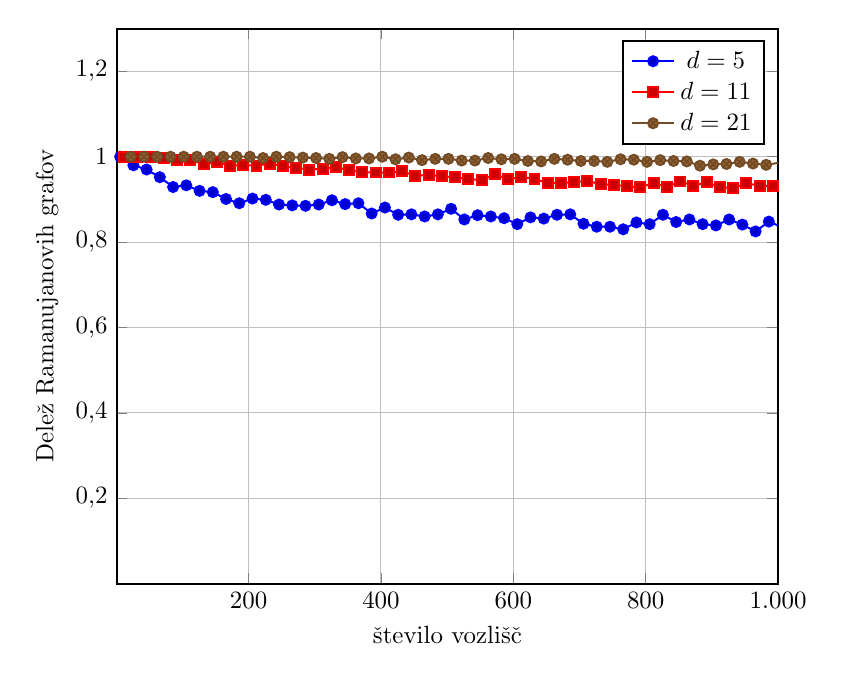
\begin{tikzpicture}[scale=0.9]
        \begin{axis}[
                xlabel={število vozlišč},
                width=0.9\textwidth,
                ylabel={Delež Ramanujanovih grafov},
                grid=major,
                ymin=0, ymax=1.3,
                xmin=1, xmax=1000,
                xtick={0,200,...,1000},
                ytick={0.2,0.4,0.6,0.8,1,1.2},
                tick label style={/pgf/number format/use comma},
                thick
            ]
            \addplot coordinates {
                (6, 1.0)
                (26, 0.98)
                (46, 0.97)
                (66, 0.952)
                (86, 0.929)
                (106, 0.933)
                (126, 0.92)
                (146, 0.917)
                (166, 0.901)
                (186, 0.891)
                (206, 0.902)
                (226, 0.899)
                (246, 0.888)
                (266, 0.886)
                (286, 0.885)
                (306, 0.888)
                (326, 0.898)
                (346, 0.889)
                (366, 0.891)
                (386, 0.867)
                (406, 0.881)
                (426, 0.864)
                (446, 0.865)
                (466, 0.86)
                (486, 0.865)
                (506, 0.878)
                (526, 0.853)
                (546, 0.863)
                (566, 0.86)
                (586, 0.856)
                (606, 0.842)
                (626, 0.858)
                (646, 0.855)
                (666, 0.864)
                (686, 0.865)
                (706, 0.843)
                (726, 0.836)
                (746, 0.836)
                (766, 0.83)
                (786, 0.846)
                (806, 0.842)
                (826, 0.864)
                (846, 0.847)
                (866, 0.853)
                (886, 0.842)
                (906, 0.839)
                (926, 0.853)
                (946, 0.841)
                (966, 0.825)
                (986, 0.848)
                (1006, 0.835)
                };
            \addlegendentry{\(d=5\)}
            \addplot coordinates {
                (12, 1.0)
                (32, 1.0)
                (52, 0.999)
                (72, 0.996)
                (92, 0.993)
                (112, 0.992)
                (132, 0.983)
                (152, 0.987)
                (172, 0.979)
                (192, 0.98)
                (212, 0.979)
                (232, 0.984)
                (252, 0.978)
                (272, 0.974)
                (292, 0.97)
                (312, 0.972)
                (332, 0.976)
                (352, 0.968)
                (372, 0.964)
                (392, 0.963)
                (412, 0.963)
                (432, 0.966)
                (452, 0.955)
                (472, 0.958)
                (492, 0.954)
                (512, 0.952)
                (532, 0.948)
                (552, 0.945)
                (572, 0.959)
                (592, 0.947)
                (612, 0.953)
                (632, 0.948)
                (652, 0.938)
                (672, 0.939)
                (692, 0.94)
                (712, 0.944)
                (732, 0.935)
                (752, 0.934)
                (772, 0.931)
                (792, 0.928)
                (812, 0.939)
                (832, 0.929)
                (852, 0.942)
                (872, 0.932)
                (892, 0.94)
                (912, 0.929)
                (932, 0.926)
                (952, 0.938)
                (972, 0.932)
                (992, 0.931)
                (1012, 0.923)
                };
                \addlegendentry{\(d=11\)}
                \addplot coordinates {
                    (22, 1.0)
                    (42, 1.0)
                    (62, 1.0)
                    (82, 1.0)
                    (102, 1.0)
                    (122, 1.0)
                    (142, 1.0)
                    (162, 1.0)
                    (182, 1.0)
                    (202, 1.0)
                    (222, 0.997)
                    (242, 1.0)
                    (262, 0.999)
                    (282, 0.998)
                    (302, 0.997)
                    (322, 0.995)
                    (342, 0.999)
                    (362, 0.996)
                    (382, 0.996)
                    (402, 1.0)
                    (422, 0.994)
                    (442, 0.998)
                    (462, 0.992)
                    (482, 0.995)
                    (502, 0.995)
                    (522, 0.991)
                    (542, 0.991)
                    (562, 0.997)
                    (582, 0.994)
                    (602, 0.995)
                    (622, 0.99)
                    (642, 0.989)
                    (662, 0.995)
                    (682, 0.993)
                    (702, 0.99)
                    (722, 0.99)
                    (742, 0.988)
                    (762, 0.994)
                    (782, 0.993)
                    (802, 0.988)
                    (822, 0.992)
                    (842, 0.99)
                    (862, 0.989)
                    (882, 0.979)
                    (902, 0.982)
                    (922, 0.983)
                    (942, 0.988)
                    (962, 0.984)
                    (982, 0.981)
                    (1002, 0.986)
                    };
                    \addlegendentry{\(d=21\)}   
        \end{axis}
    \end{tikzpicture}
    \caption{Graf deleža Ramanujanovih grafov od 1 do 300}
\end{figure}
\begin{figure}[H]
    \centering
    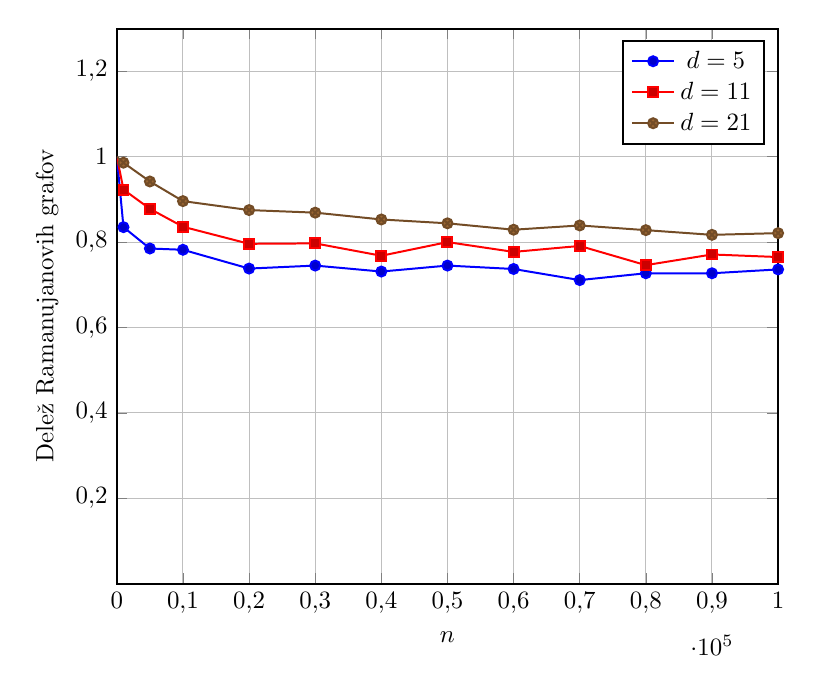
\begin{tikzpicture}[scale=0.9]
        \begin{axis}[
                xlabel={$n$},
                width=0.9\textwidth,
                ylabel={Delež Ramanujanovih grafov},
                grid=major,
                ymin=0, ymax=1.3,
                xmin=1, xmax=100000,
                xtick={0,10000,...,100000},
                ytick={0.2,0.4,0.6,0.8,1,1.2},
                tick label style={/pgf/number format/use comma},
                thick
            ]
            \addplot coordinates {
                (0, 1.0)
                (1006, 0.835)
                (5000, 0.785)
                (10000, 0.782)
                (20000, 0.738)
                (30000, 0.745)
                (40000, 0.731)
                (50000, 0.745)
                (60000, 0.737)
                (70000, 0.711)
                (80000, 0.727)
                (90000, 0.727)
                (100000, 0.736)
                };
                \addlegendentry{\(d=5\)}
            \addplot coordinates {
                (0, 1.0)
                (1012, 0.923)
                (5000, 0.878)
                (10000, 0.836)
                (20000, 0.796)
                (30000, 0.797)
                (40000, 0.768)
                (50000, 0.8)
                (60000, 0.777)
                (70000, 0.791)
                (80000, 0.746)
                (90000, 0.771)
                (100000, 0.765)
                };
                \addlegendentry{\(d=11\)}
            \addplot coordinates {
                (0, 1.0)
                (1002, 0.986)
                (5000, 0.942)
                (10000, 0.896)
                (20000, 0.875)
                (30000, 0.869)
                (40000, 0.853)
                (50000, 0.844)
                (60000, 0.829)
                (70000, 0.839)
                (80000, 0.828)
                (90000, 0.817)
                (100000, 0.821)
                };
                \addlegendentry{\(d=21\)}
    \end{axis}
    \end{tikzpicture}
    \caption{Graf deleža Ramanujanovih grafov od 10000 do 100000}
\end{figure}
Na grafih vidimo, da se delež Ramanujanovih grafov z večanjem števila vozlišč zmanjšuje. Vidimo pa tudi, da se ta delež zmanjšuje hitreje pri nižjih stopnjah regularnosti. Najpomembnejše pa je, da se ta delež ne približuje \(0\), ne glede na stopnjo regularnosti; na grafih vidimo, da se delež približuje približno \(70\%\), vendar je težko trditi, saj kljub velikemu številu vozlišč še vedno ni vidne končne konvergence. Dokaza za to trditev si ne bomo ogledali, je bilo pa nedavno dokazano, da je delež Ramanujanovih grafov asimptotično neodvisen od stopnje regularnosti in se približuje približno \(69\%\) \cite{huang2024ramanujanpropertyedgeuniversality}. Ključni del dokaza je bil, da so izračunali, da se porazdelitev največje netrivialne lastne vrednosti približuje Tracy-Widomovi porazdelitvi. Za to porazdelitev pa lahko preverimo, kolikšno maso ima pod Ramanujanovo mejo. Omenjeni članek predstavlja pomemben preboj v teoriji Ramanujanovih grafov, saj je bila porazdelitev lastnih vrednosti, prav tako pa delež Ramanujanovih grafov, dolgo obstoječ odprt problem.

\begin{figure}[H]
    \begin{center}
        %% Creator: Matplotlib, PGF backend
%%
%% To include the figure in your LaTeX document, write
%%   \input{<filename>.pgf}
%%
%% Make sure the required packages are loaded in your preamble
%%   \usepackage{pgf}
%%
%% Also ensure that all the required font packages are loaded; for instance,
%% the lmodern package is sometimes necessary when using math font.
%%   \usepackage{lmodern}
%%
%% Figures using additional raster images can only be included by \input if
%% they are in the same directory as the main LaTeX file. For loading figures
%% from other directories you can use the `import` package
%%   \usepackage{import}
%%
%% and then include the figures with
%%   \import{<path to file>}{<filename>.pgf}
%%
%% Matplotlib used the following preamble
%%   \def\mathdefault#1{#1}
%%   \everymath=\expandafter{\the\everymath\displaystyle}
%%   \IfFileExists{scrextend.sty}{
%%     \usepackage[fontsize=10.000000pt]{scrextend}
%%   }{
%%     \renewcommand{\normalsize}{\fontsize{10.000000}{12.000000}\selectfont}
%%     \normalsize
%%   }
%%   
%%   \makeatletter\@ifpackageloaded{underscore}{}{\usepackage[strings]{underscore}}\makeatother
%%
\begingroup%
\makeatletter%
\begin{pgfpicture}%
\pgfpathrectangle{\pgfpointorigin}{\pgfqpoint{5.906660in}{6.000000in}}%
\pgfusepath{use as bounding box, clip}%
\begin{pgfscope}%
\pgfsetbuttcap%
\pgfsetmiterjoin%
\definecolor{currentfill}{rgb}{1.000000,1.000000,1.000000}%
\pgfsetfillcolor{currentfill}%
\pgfsetlinewidth{0.000000pt}%
\definecolor{currentstroke}{rgb}{1.000000,1.000000,1.000000}%
\pgfsetstrokecolor{currentstroke}%
\pgfsetdash{}{0pt}%
\pgfpathmoveto{\pgfqpoint{0.000000in}{0.000000in}}%
\pgfpathlineto{\pgfqpoint{5.906660in}{0.000000in}}%
\pgfpathlineto{\pgfqpoint{5.906660in}{6.000000in}}%
\pgfpathlineto{\pgfqpoint{0.000000in}{6.000000in}}%
\pgfpathlineto{\pgfqpoint{0.000000in}{0.000000in}}%
\pgfpathclose%
\pgfusepath{fill}%
\end{pgfscope}%
\begin{pgfscope}%
\pgfsetbuttcap%
\pgfsetmiterjoin%
\definecolor{currentfill}{rgb}{1.000000,1.000000,1.000000}%
\pgfsetfillcolor{currentfill}%
\pgfsetlinewidth{0.000000pt}%
\definecolor{currentstroke}{rgb}{0.000000,0.000000,0.000000}%
\pgfsetstrokecolor{currentstroke}%
\pgfsetstrokeopacity{0.000000}%
\pgfsetdash{}{0pt}%
\pgfpathmoveto{\pgfqpoint{0.819028in}{0.582778in}}%
\pgfpathlineto{\pgfqpoint{5.756660in}{0.582778in}}%
\pgfpathlineto{\pgfqpoint{5.756660in}{5.850000in}}%
\pgfpathlineto{\pgfqpoint{0.819028in}{5.850000in}}%
\pgfpathlineto{\pgfqpoint{0.819028in}{0.582778in}}%
\pgfpathclose%
\pgfusepath{fill}%
\end{pgfscope}%
\begin{pgfscope}%
\pgfpathrectangle{\pgfqpoint{0.819028in}{0.582778in}}{\pgfqpoint{4.937632in}{5.267222in}}%
\pgfusepath{clip}%
\pgfsetbuttcap%
\pgfsetmiterjoin%
\definecolor{currentfill}{rgb}{0.121569,0.466667,0.705882}%
\pgfsetfillcolor{currentfill}%
\pgfsetfillopacity{0.700000}%
\pgfsetlinewidth{1.003750pt}%
\definecolor{currentstroke}{rgb}{0.000000,0.000000,0.000000}%
\pgfsetstrokecolor{currentstroke}%
\pgfsetstrokeopacity{0.700000}%
\pgfsetdash{}{0pt}%
\pgfpathmoveto{\pgfqpoint{1.043466in}{0.582778in}}%
\pgfpathlineto{\pgfqpoint{1.193091in}{0.582778in}}%
\pgfpathlineto{\pgfqpoint{1.193091in}{0.605253in}}%
\pgfpathlineto{\pgfqpoint{1.043466in}{0.605253in}}%
\pgfpathlineto{\pgfqpoint{1.043466in}{0.582778in}}%
\pgfpathclose%
\pgfusepath{stroke,fill}%
\end{pgfscope}%
\begin{pgfscope}%
\pgfpathrectangle{\pgfqpoint{0.819028in}{0.582778in}}{\pgfqpoint{4.937632in}{5.267222in}}%
\pgfusepath{clip}%
\pgfsetbuttcap%
\pgfsetmiterjoin%
\definecolor{currentfill}{rgb}{0.121569,0.466667,0.705882}%
\pgfsetfillcolor{currentfill}%
\pgfsetfillopacity{0.700000}%
\pgfsetlinewidth{1.003750pt}%
\definecolor{currentstroke}{rgb}{0.000000,0.000000,0.000000}%
\pgfsetstrokecolor{currentstroke}%
\pgfsetstrokeopacity{0.700000}%
\pgfsetdash{}{0pt}%
\pgfpathmoveto{\pgfqpoint{1.193091in}{0.582778in}}%
\pgfpathlineto{\pgfqpoint{1.342716in}{0.582778in}}%
\pgfpathlineto{\pgfqpoint{1.342716in}{0.650203in}}%
\pgfpathlineto{\pgfqpoint{1.193091in}{0.650203in}}%
\pgfpathlineto{\pgfqpoint{1.193091in}{0.582778in}}%
\pgfpathclose%
\pgfusepath{stroke,fill}%
\end{pgfscope}%
\begin{pgfscope}%
\pgfpathrectangle{\pgfqpoint{0.819028in}{0.582778in}}{\pgfqpoint{4.937632in}{5.267222in}}%
\pgfusepath{clip}%
\pgfsetbuttcap%
\pgfsetmiterjoin%
\definecolor{currentfill}{rgb}{0.121569,0.466667,0.705882}%
\pgfsetfillcolor{currentfill}%
\pgfsetfillopacity{0.700000}%
\pgfsetlinewidth{1.003750pt}%
\definecolor{currentstroke}{rgb}{0.000000,0.000000,0.000000}%
\pgfsetstrokecolor{currentstroke}%
\pgfsetstrokeopacity{0.700000}%
\pgfsetdash{}{0pt}%
\pgfpathmoveto{\pgfqpoint{1.342716in}{0.582778in}}%
\pgfpathlineto{\pgfqpoint{1.492341in}{0.582778in}}%
\pgfpathlineto{\pgfqpoint{1.492341in}{0.758082in}}%
\pgfpathlineto{\pgfqpoint{1.342716in}{0.758082in}}%
\pgfpathlineto{\pgfqpoint{1.342716in}{0.582778in}}%
\pgfpathclose%
\pgfusepath{stroke,fill}%
\end{pgfscope}%
\begin{pgfscope}%
\pgfpathrectangle{\pgfqpoint{0.819028in}{0.582778in}}{\pgfqpoint{4.937632in}{5.267222in}}%
\pgfusepath{clip}%
\pgfsetbuttcap%
\pgfsetmiterjoin%
\definecolor{currentfill}{rgb}{0.121569,0.466667,0.705882}%
\pgfsetfillcolor{currentfill}%
\pgfsetfillopacity{0.700000}%
\pgfsetlinewidth{1.003750pt}%
\definecolor{currentstroke}{rgb}{0.000000,0.000000,0.000000}%
\pgfsetstrokecolor{currentstroke}%
\pgfsetstrokeopacity{0.700000}%
\pgfsetdash{}{0pt}%
\pgfpathmoveto{\pgfqpoint{1.492341in}{0.582778in}}%
\pgfpathlineto{\pgfqpoint{1.641966in}{0.582778in}}%
\pgfpathlineto{\pgfqpoint{1.641966in}{1.077226in}}%
\pgfpathlineto{\pgfqpoint{1.492341in}{1.077226in}}%
\pgfpathlineto{\pgfqpoint{1.492341in}{0.582778in}}%
\pgfpathclose%
\pgfusepath{stroke,fill}%
\end{pgfscope}%
\begin{pgfscope}%
\pgfpathrectangle{\pgfqpoint{0.819028in}{0.582778in}}{\pgfqpoint{4.937632in}{5.267222in}}%
\pgfusepath{clip}%
\pgfsetbuttcap%
\pgfsetmiterjoin%
\definecolor{currentfill}{rgb}{0.121569,0.466667,0.705882}%
\pgfsetfillcolor{currentfill}%
\pgfsetfillopacity{0.700000}%
\pgfsetlinewidth{1.003750pt}%
\definecolor{currentstroke}{rgb}{0.000000,0.000000,0.000000}%
\pgfsetstrokecolor{currentstroke}%
\pgfsetstrokeopacity{0.700000}%
\pgfsetdash{}{0pt}%
\pgfpathmoveto{\pgfqpoint{1.641966in}{0.582778in}}%
\pgfpathlineto{\pgfqpoint{1.791592in}{0.582778in}}%
\pgfpathlineto{\pgfqpoint{1.791592in}{1.670564in}}%
\pgfpathlineto{\pgfqpoint{1.641966in}{1.670564in}}%
\pgfpathlineto{\pgfqpoint{1.641966in}{0.582778in}}%
\pgfpathclose%
\pgfusepath{stroke,fill}%
\end{pgfscope}%
\begin{pgfscope}%
\pgfpathrectangle{\pgfqpoint{0.819028in}{0.582778in}}{\pgfqpoint{4.937632in}{5.267222in}}%
\pgfusepath{clip}%
\pgfsetbuttcap%
\pgfsetmiterjoin%
\definecolor{currentfill}{rgb}{0.121569,0.466667,0.705882}%
\pgfsetfillcolor{currentfill}%
\pgfsetfillopacity{0.700000}%
\pgfsetlinewidth{1.003750pt}%
\definecolor{currentstroke}{rgb}{0.000000,0.000000,0.000000}%
\pgfsetstrokecolor{currentstroke}%
\pgfsetstrokeopacity{0.700000}%
\pgfsetdash{}{0pt}%
\pgfpathmoveto{\pgfqpoint{1.791592in}{0.582778in}}%
\pgfpathlineto{\pgfqpoint{1.941217in}{0.582778in}}%
\pgfpathlineto{\pgfqpoint{1.941217in}{2.227942in}}%
\pgfpathlineto{\pgfqpoint{1.791592in}{2.227942in}}%
\pgfpathlineto{\pgfqpoint{1.791592in}{0.582778in}}%
\pgfpathclose%
\pgfusepath{stroke,fill}%
\end{pgfscope}%
\begin{pgfscope}%
\pgfpathrectangle{\pgfqpoint{0.819028in}{0.582778in}}{\pgfqpoint{4.937632in}{5.267222in}}%
\pgfusepath{clip}%
\pgfsetbuttcap%
\pgfsetmiterjoin%
\definecolor{currentfill}{rgb}{0.121569,0.466667,0.705882}%
\pgfsetfillcolor{currentfill}%
\pgfsetfillopacity{0.700000}%
\pgfsetlinewidth{1.003750pt}%
\definecolor{currentstroke}{rgb}{0.000000,0.000000,0.000000}%
\pgfsetstrokecolor{currentstroke}%
\pgfsetstrokeopacity{0.700000}%
\pgfsetdash{}{0pt}%
\pgfpathmoveto{\pgfqpoint{1.941217in}{0.582778in}}%
\pgfpathlineto{\pgfqpoint{2.090842in}{0.582778in}}%
\pgfpathlineto{\pgfqpoint{2.090842in}{3.167394in}}%
\pgfpathlineto{\pgfqpoint{1.941217in}{3.167394in}}%
\pgfpathlineto{\pgfqpoint{1.941217in}{0.582778in}}%
\pgfpathclose%
\pgfusepath{stroke,fill}%
\end{pgfscope}%
\begin{pgfscope}%
\pgfpathrectangle{\pgfqpoint{0.819028in}{0.582778in}}{\pgfqpoint{4.937632in}{5.267222in}}%
\pgfusepath{clip}%
\pgfsetbuttcap%
\pgfsetmiterjoin%
\definecolor{currentfill}{rgb}{0.121569,0.466667,0.705882}%
\pgfsetfillcolor{currentfill}%
\pgfsetfillopacity{0.700000}%
\pgfsetlinewidth{1.003750pt}%
\definecolor{currentstroke}{rgb}{0.000000,0.000000,0.000000}%
\pgfsetstrokecolor{currentstroke}%
\pgfsetstrokeopacity{0.700000}%
\pgfsetdash{}{0pt}%
\pgfpathmoveto{\pgfqpoint{2.090842in}{0.582778in}}%
\pgfpathlineto{\pgfqpoint{2.240467in}{0.582778in}}%
\pgfpathlineto{\pgfqpoint{2.240467in}{3.864116in}}%
\pgfpathlineto{\pgfqpoint{2.090842in}{3.864116in}}%
\pgfpathlineto{\pgfqpoint{2.090842in}{0.582778in}}%
\pgfpathclose%
\pgfusepath{stroke,fill}%
\end{pgfscope}%
\begin{pgfscope}%
\pgfpathrectangle{\pgfqpoint{0.819028in}{0.582778in}}{\pgfqpoint{4.937632in}{5.267222in}}%
\pgfusepath{clip}%
\pgfsetbuttcap%
\pgfsetmiterjoin%
\definecolor{currentfill}{rgb}{0.121569,0.466667,0.705882}%
\pgfsetfillcolor{currentfill}%
\pgfsetfillopacity{0.700000}%
\pgfsetlinewidth{1.003750pt}%
\definecolor{currentstroke}{rgb}{0.000000,0.000000,0.000000}%
\pgfsetstrokecolor{currentstroke}%
\pgfsetstrokeopacity{0.700000}%
\pgfsetdash{}{0pt}%
\pgfpathmoveto{\pgfqpoint{2.240467in}{0.582778in}}%
\pgfpathlineto{\pgfqpoint{2.390093in}{0.582778in}}%
\pgfpathlineto{\pgfqpoint{2.390093in}{4.763113in}}%
\pgfpathlineto{\pgfqpoint{2.240467in}{4.763113in}}%
\pgfpathlineto{\pgfqpoint{2.240467in}{0.582778in}}%
\pgfpathclose%
\pgfusepath{stroke,fill}%
\end{pgfscope}%
\begin{pgfscope}%
\pgfpathrectangle{\pgfqpoint{0.819028in}{0.582778in}}{\pgfqpoint{4.937632in}{5.267222in}}%
\pgfusepath{clip}%
\pgfsetbuttcap%
\pgfsetmiterjoin%
\definecolor{currentfill}{rgb}{0.121569,0.466667,0.705882}%
\pgfsetfillcolor{currentfill}%
\pgfsetfillopacity{0.700000}%
\pgfsetlinewidth{1.003750pt}%
\definecolor{currentstroke}{rgb}{0.000000,0.000000,0.000000}%
\pgfsetstrokecolor{currentstroke}%
\pgfsetstrokeopacity{0.700000}%
\pgfsetdash{}{0pt}%
\pgfpathmoveto{\pgfqpoint{2.390093in}{0.582778in}}%
\pgfpathlineto{\pgfqpoint{2.539718in}{0.582778in}}%
\pgfpathlineto{\pgfqpoint{2.539718in}{4.830538in}}%
\pgfpathlineto{\pgfqpoint{2.390093in}{4.830538in}}%
\pgfpathlineto{\pgfqpoint{2.390093in}{0.582778in}}%
\pgfpathclose%
\pgfusepath{stroke,fill}%
\end{pgfscope}%
\begin{pgfscope}%
\pgfpathrectangle{\pgfqpoint{0.819028in}{0.582778in}}{\pgfqpoint{4.937632in}{5.267222in}}%
\pgfusepath{clip}%
\pgfsetbuttcap%
\pgfsetmiterjoin%
\definecolor{currentfill}{rgb}{0.121569,0.466667,0.705882}%
\pgfsetfillcolor{currentfill}%
\pgfsetfillopacity{0.700000}%
\pgfsetlinewidth{1.003750pt}%
\definecolor{currentstroke}{rgb}{0.000000,0.000000,0.000000}%
\pgfsetstrokecolor{currentstroke}%
\pgfsetstrokeopacity{0.700000}%
\pgfsetdash{}{0pt}%
\pgfpathmoveto{\pgfqpoint{2.539718in}{0.582778in}}%
\pgfpathlineto{\pgfqpoint{2.689343in}{0.582778in}}%
\pgfpathlineto{\pgfqpoint{2.689343in}{5.599180in}}%
\pgfpathlineto{\pgfqpoint{2.539718in}{5.599180in}}%
\pgfpathlineto{\pgfqpoint{2.539718in}{0.582778in}}%
\pgfpathclose%
\pgfusepath{stroke,fill}%
\end{pgfscope}%
\begin{pgfscope}%
\pgfpathrectangle{\pgfqpoint{0.819028in}{0.582778in}}{\pgfqpoint{4.937632in}{5.267222in}}%
\pgfusepath{clip}%
\pgfsetbuttcap%
\pgfsetmiterjoin%
\definecolor{currentfill}{rgb}{0.121569,0.466667,0.705882}%
\pgfsetfillcolor{currentfill}%
\pgfsetfillopacity{0.700000}%
\pgfsetlinewidth{1.003750pt}%
\definecolor{currentstroke}{rgb}{0.000000,0.000000,0.000000}%
\pgfsetstrokecolor{currentstroke}%
\pgfsetstrokeopacity{0.700000}%
\pgfsetdash{}{0pt}%
\pgfpathmoveto{\pgfqpoint{2.689343in}{0.582778in}}%
\pgfpathlineto{\pgfqpoint{2.838968in}{0.582778in}}%
\pgfpathlineto{\pgfqpoint{2.838968in}{5.369936in}}%
\pgfpathlineto{\pgfqpoint{2.689343in}{5.369936in}}%
\pgfpathlineto{\pgfqpoint{2.689343in}{0.582778in}}%
\pgfpathclose%
\pgfusepath{stroke,fill}%
\end{pgfscope}%
\begin{pgfscope}%
\pgfpathrectangle{\pgfqpoint{0.819028in}{0.582778in}}{\pgfqpoint{4.937632in}{5.267222in}}%
\pgfusepath{clip}%
\pgfsetbuttcap%
\pgfsetmiterjoin%
\definecolor{currentfill}{rgb}{0.121569,0.466667,0.705882}%
\pgfsetfillcolor{currentfill}%
\pgfsetfillopacity{0.700000}%
\pgfsetlinewidth{1.003750pt}%
\definecolor{currentstroke}{rgb}{0.000000,0.000000,0.000000}%
\pgfsetstrokecolor{currentstroke}%
\pgfsetstrokeopacity{0.700000}%
\pgfsetdash{}{0pt}%
\pgfpathmoveto{\pgfqpoint{2.838968in}{0.582778in}}%
\pgfpathlineto{\pgfqpoint{2.988593in}{0.582778in}}%
\pgfpathlineto{\pgfqpoint{2.988593in}{4.965387in}}%
\pgfpathlineto{\pgfqpoint{2.838968in}{4.965387in}}%
\pgfpathlineto{\pgfqpoint{2.838968in}{0.582778in}}%
\pgfpathclose%
\pgfusepath{stroke,fill}%
\end{pgfscope}%
\begin{pgfscope}%
\pgfpathrectangle{\pgfqpoint{0.819028in}{0.582778in}}{\pgfqpoint{4.937632in}{5.267222in}}%
\pgfusepath{clip}%
\pgfsetbuttcap%
\pgfsetmiterjoin%
\definecolor{currentfill}{rgb}{0.121569,0.466667,0.705882}%
\pgfsetfillcolor{currentfill}%
\pgfsetfillopacity{0.700000}%
\pgfsetlinewidth{1.003750pt}%
\definecolor{currentstroke}{rgb}{0.000000,0.000000,0.000000}%
\pgfsetstrokecolor{currentstroke}%
\pgfsetstrokeopacity{0.700000}%
\pgfsetdash{}{0pt}%
\pgfpathmoveto{\pgfqpoint{2.988593in}{0.582778in}}%
\pgfpathlineto{\pgfqpoint{3.138219in}{0.582778in}}%
\pgfpathlineto{\pgfqpoint{3.138219in}{4.097855in}}%
\pgfpathlineto{\pgfqpoint{2.988593in}{4.097855in}}%
\pgfpathlineto{\pgfqpoint{2.988593in}{0.582778in}}%
\pgfpathclose%
\pgfusepath{stroke,fill}%
\end{pgfscope}%
\begin{pgfscope}%
\pgfpathrectangle{\pgfqpoint{0.819028in}{0.582778in}}{\pgfqpoint{4.937632in}{5.267222in}}%
\pgfusepath{clip}%
\pgfsetbuttcap%
\pgfsetmiterjoin%
\definecolor{currentfill}{rgb}{0.121569,0.466667,0.705882}%
\pgfsetfillcolor{currentfill}%
\pgfsetfillopacity{0.700000}%
\pgfsetlinewidth{1.003750pt}%
\definecolor{currentstroke}{rgb}{0.000000,0.000000,0.000000}%
\pgfsetstrokecolor{currentstroke}%
\pgfsetstrokeopacity{0.700000}%
\pgfsetdash{}{0pt}%
\pgfpathmoveto{\pgfqpoint{3.138219in}{0.582778in}}%
\pgfpathlineto{\pgfqpoint{3.287844in}{0.582778in}}%
\pgfpathlineto{\pgfqpoint{3.287844in}{3.419113in}}%
\pgfpathlineto{\pgfqpoint{3.138219in}{3.419113in}}%
\pgfpathlineto{\pgfqpoint{3.138219in}{0.582778in}}%
\pgfpathclose%
\pgfusepath{stroke,fill}%
\end{pgfscope}%
\begin{pgfscope}%
\pgfpathrectangle{\pgfqpoint{0.819028in}{0.582778in}}{\pgfqpoint{4.937632in}{5.267222in}}%
\pgfusepath{clip}%
\pgfsetbuttcap%
\pgfsetmiterjoin%
\definecolor{currentfill}{rgb}{0.121569,0.466667,0.705882}%
\pgfsetfillcolor{currentfill}%
\pgfsetfillopacity{0.700000}%
\pgfsetlinewidth{1.003750pt}%
\definecolor{currentstroke}{rgb}{0.000000,0.000000,0.000000}%
\pgfsetstrokecolor{currentstroke}%
\pgfsetstrokeopacity{0.700000}%
\pgfsetdash{}{0pt}%
\pgfpathmoveto{\pgfqpoint{3.287844in}{0.582778in}}%
\pgfpathlineto{\pgfqpoint{3.437469in}{0.582778in}}%
\pgfpathlineto{\pgfqpoint{3.437469in}{2.619006in}}%
\pgfpathlineto{\pgfqpoint{3.287844in}{2.619006in}}%
\pgfpathlineto{\pgfqpoint{3.287844in}{0.582778in}}%
\pgfpathclose%
\pgfusepath{stroke,fill}%
\end{pgfscope}%
\begin{pgfscope}%
\pgfpathrectangle{\pgfqpoint{0.819028in}{0.582778in}}{\pgfqpoint{4.937632in}{5.267222in}}%
\pgfusepath{clip}%
\pgfsetbuttcap%
\pgfsetmiterjoin%
\definecolor{currentfill}{rgb}{0.121569,0.466667,0.705882}%
\pgfsetfillcolor{currentfill}%
\pgfsetfillopacity{0.700000}%
\pgfsetlinewidth{1.003750pt}%
\definecolor{currentstroke}{rgb}{0.000000,0.000000,0.000000}%
\pgfsetstrokecolor{currentstroke}%
\pgfsetstrokeopacity{0.700000}%
\pgfsetdash{}{0pt}%
\pgfpathmoveto{\pgfqpoint{3.437469in}{0.582778in}}%
\pgfpathlineto{\pgfqpoint{3.587094in}{0.582778in}}%
\pgfpathlineto{\pgfqpoint{3.587094in}{2.138042in}}%
\pgfpathlineto{\pgfqpoint{3.437469in}{2.138042in}}%
\pgfpathlineto{\pgfqpoint{3.437469in}{0.582778in}}%
\pgfpathclose%
\pgfusepath{stroke,fill}%
\end{pgfscope}%
\begin{pgfscope}%
\pgfpathrectangle{\pgfqpoint{0.819028in}{0.582778in}}{\pgfqpoint{4.937632in}{5.267222in}}%
\pgfusepath{clip}%
\pgfsetbuttcap%
\pgfsetmiterjoin%
\definecolor{currentfill}{rgb}{0.121569,0.466667,0.705882}%
\pgfsetfillcolor{currentfill}%
\pgfsetfillopacity{0.700000}%
\pgfsetlinewidth{1.003750pt}%
\definecolor{currentstroke}{rgb}{0.000000,0.000000,0.000000}%
\pgfsetstrokecolor{currentstroke}%
\pgfsetstrokeopacity{0.700000}%
\pgfsetdash{}{0pt}%
\pgfpathmoveto{\pgfqpoint{3.587094in}{0.582778in}}%
\pgfpathlineto{\pgfqpoint{3.736720in}{0.582778in}}%
\pgfpathlineto{\pgfqpoint{3.736720in}{1.661574in}}%
\pgfpathlineto{\pgfqpoint{3.587094in}{1.661574in}}%
\pgfpathlineto{\pgfqpoint{3.587094in}{0.582778in}}%
\pgfpathclose%
\pgfusepath{stroke,fill}%
\end{pgfscope}%
\begin{pgfscope}%
\pgfpathrectangle{\pgfqpoint{0.819028in}{0.582778in}}{\pgfqpoint{4.937632in}{5.267222in}}%
\pgfusepath{clip}%
\pgfsetbuttcap%
\pgfsetmiterjoin%
\definecolor{currentfill}{rgb}{0.121569,0.466667,0.705882}%
\pgfsetfillcolor{currentfill}%
\pgfsetfillopacity{0.700000}%
\pgfsetlinewidth{1.003750pt}%
\definecolor{currentstroke}{rgb}{0.000000,0.000000,0.000000}%
\pgfsetstrokecolor{currentstroke}%
\pgfsetstrokeopacity{0.700000}%
\pgfsetdash{}{0pt}%
\pgfpathmoveto{\pgfqpoint{3.736720in}{0.582778in}}%
\pgfpathlineto{\pgfqpoint{3.886345in}{0.582778in}}%
\pgfpathlineto{\pgfqpoint{3.886345in}{1.310965in}}%
\pgfpathlineto{\pgfqpoint{3.736720in}{1.310965in}}%
\pgfpathlineto{\pgfqpoint{3.736720in}{0.582778in}}%
\pgfpathclose%
\pgfusepath{stroke,fill}%
\end{pgfscope}%
\begin{pgfscope}%
\pgfpathrectangle{\pgfqpoint{0.819028in}{0.582778in}}{\pgfqpoint{4.937632in}{5.267222in}}%
\pgfusepath{clip}%
\pgfsetbuttcap%
\pgfsetmiterjoin%
\definecolor{currentfill}{rgb}{0.121569,0.466667,0.705882}%
\pgfsetfillcolor{currentfill}%
\pgfsetfillopacity{0.700000}%
\pgfsetlinewidth{1.003750pt}%
\definecolor{currentstroke}{rgb}{0.000000,0.000000,0.000000}%
\pgfsetstrokecolor{currentstroke}%
\pgfsetstrokeopacity{0.700000}%
\pgfsetdash{}{0pt}%
\pgfpathmoveto{\pgfqpoint{3.886345in}{0.582778in}}%
\pgfpathlineto{\pgfqpoint{4.035970in}{0.582778in}}%
\pgfpathlineto{\pgfqpoint{4.035970in}{1.077226in}}%
\pgfpathlineto{\pgfqpoint{3.886345in}{1.077226in}}%
\pgfpathlineto{\pgfqpoint{3.886345in}{0.582778in}}%
\pgfpathclose%
\pgfusepath{stroke,fill}%
\end{pgfscope}%
\begin{pgfscope}%
\pgfpathrectangle{\pgfqpoint{0.819028in}{0.582778in}}{\pgfqpoint{4.937632in}{5.267222in}}%
\pgfusepath{clip}%
\pgfsetbuttcap%
\pgfsetmiterjoin%
\definecolor{currentfill}{rgb}{0.121569,0.466667,0.705882}%
\pgfsetfillcolor{currentfill}%
\pgfsetfillopacity{0.700000}%
\pgfsetlinewidth{1.003750pt}%
\definecolor{currentstroke}{rgb}{0.000000,0.000000,0.000000}%
\pgfsetstrokecolor{currentstroke}%
\pgfsetstrokeopacity{0.700000}%
\pgfsetdash{}{0pt}%
\pgfpathmoveto{\pgfqpoint{4.035970in}{0.582778in}}%
\pgfpathlineto{\pgfqpoint{4.185595in}{0.582778in}}%
\pgfpathlineto{\pgfqpoint{4.185595in}{0.892932in}}%
\pgfpathlineto{\pgfqpoint{4.035970in}{0.892932in}}%
\pgfpathlineto{\pgfqpoint{4.035970in}{0.582778in}}%
\pgfpathclose%
\pgfusepath{stroke,fill}%
\end{pgfscope}%
\begin{pgfscope}%
\pgfpathrectangle{\pgfqpoint{0.819028in}{0.582778in}}{\pgfqpoint{4.937632in}{5.267222in}}%
\pgfusepath{clip}%
\pgfsetbuttcap%
\pgfsetmiterjoin%
\definecolor{currentfill}{rgb}{0.121569,0.466667,0.705882}%
\pgfsetfillcolor{currentfill}%
\pgfsetfillopacity{0.700000}%
\pgfsetlinewidth{1.003750pt}%
\definecolor{currentstroke}{rgb}{0.000000,0.000000,0.000000}%
\pgfsetstrokecolor{currentstroke}%
\pgfsetstrokeopacity{0.700000}%
\pgfsetdash{}{0pt}%
\pgfpathmoveto{\pgfqpoint{4.185595in}{0.582778in}}%
\pgfpathlineto{\pgfqpoint{4.335220in}{0.582778in}}%
\pgfpathlineto{\pgfqpoint{4.335220in}{0.758082in}}%
\pgfpathlineto{\pgfqpoint{4.185595in}{0.758082in}}%
\pgfpathlineto{\pgfqpoint{4.185595in}{0.582778in}}%
\pgfpathclose%
\pgfusepath{stroke,fill}%
\end{pgfscope}%
\begin{pgfscope}%
\pgfpathrectangle{\pgfqpoint{0.819028in}{0.582778in}}{\pgfqpoint{4.937632in}{5.267222in}}%
\pgfusepath{clip}%
\pgfsetbuttcap%
\pgfsetmiterjoin%
\definecolor{currentfill}{rgb}{0.121569,0.466667,0.705882}%
\pgfsetfillcolor{currentfill}%
\pgfsetfillopacity{0.700000}%
\pgfsetlinewidth{1.003750pt}%
\definecolor{currentstroke}{rgb}{0.000000,0.000000,0.000000}%
\pgfsetstrokecolor{currentstroke}%
\pgfsetstrokeopacity{0.700000}%
\pgfsetdash{}{0pt}%
\pgfpathmoveto{\pgfqpoint{4.335220in}{0.582778in}}%
\pgfpathlineto{\pgfqpoint{4.484846in}{0.582778in}}%
\pgfpathlineto{\pgfqpoint{4.484846in}{0.722122in}}%
\pgfpathlineto{\pgfqpoint{4.335220in}{0.722122in}}%
\pgfpathlineto{\pgfqpoint{4.335220in}{0.582778in}}%
\pgfpathclose%
\pgfusepath{stroke,fill}%
\end{pgfscope}%
\begin{pgfscope}%
\pgfpathrectangle{\pgfqpoint{0.819028in}{0.582778in}}{\pgfqpoint{4.937632in}{5.267222in}}%
\pgfusepath{clip}%
\pgfsetbuttcap%
\pgfsetmiterjoin%
\definecolor{currentfill}{rgb}{0.121569,0.466667,0.705882}%
\pgfsetfillcolor{currentfill}%
\pgfsetfillopacity{0.700000}%
\pgfsetlinewidth{1.003750pt}%
\definecolor{currentstroke}{rgb}{0.000000,0.000000,0.000000}%
\pgfsetstrokecolor{currentstroke}%
\pgfsetstrokeopacity{0.700000}%
\pgfsetdash{}{0pt}%
\pgfpathmoveto{\pgfqpoint{4.484846in}{0.582778in}}%
\pgfpathlineto{\pgfqpoint{4.634471in}{0.582778in}}%
\pgfpathlineto{\pgfqpoint{4.634471in}{0.618738in}}%
\pgfpathlineto{\pgfqpoint{4.484846in}{0.618738in}}%
\pgfpathlineto{\pgfqpoint{4.484846in}{0.582778in}}%
\pgfpathclose%
\pgfusepath{stroke,fill}%
\end{pgfscope}%
\begin{pgfscope}%
\pgfpathrectangle{\pgfqpoint{0.819028in}{0.582778in}}{\pgfqpoint{4.937632in}{5.267222in}}%
\pgfusepath{clip}%
\pgfsetbuttcap%
\pgfsetmiterjoin%
\definecolor{currentfill}{rgb}{0.121569,0.466667,0.705882}%
\pgfsetfillcolor{currentfill}%
\pgfsetfillopacity{0.700000}%
\pgfsetlinewidth{1.003750pt}%
\definecolor{currentstroke}{rgb}{0.000000,0.000000,0.000000}%
\pgfsetstrokecolor{currentstroke}%
\pgfsetstrokeopacity{0.700000}%
\pgfsetdash{}{0pt}%
\pgfpathmoveto{\pgfqpoint{4.634471in}{0.582778in}}%
\pgfpathlineto{\pgfqpoint{4.784096in}{0.582778in}}%
\pgfpathlineto{\pgfqpoint{4.784096in}{0.623233in}}%
\pgfpathlineto{\pgfqpoint{4.634471in}{0.623233in}}%
\pgfpathlineto{\pgfqpoint{4.634471in}{0.582778in}}%
\pgfpathclose%
\pgfusepath{stroke,fill}%
\end{pgfscope}%
\begin{pgfscope}%
\pgfpathrectangle{\pgfqpoint{0.819028in}{0.582778in}}{\pgfqpoint{4.937632in}{5.267222in}}%
\pgfusepath{clip}%
\pgfsetbuttcap%
\pgfsetmiterjoin%
\definecolor{currentfill}{rgb}{0.121569,0.466667,0.705882}%
\pgfsetfillcolor{currentfill}%
\pgfsetfillopacity{0.700000}%
\pgfsetlinewidth{1.003750pt}%
\definecolor{currentstroke}{rgb}{0.000000,0.000000,0.000000}%
\pgfsetstrokecolor{currentstroke}%
\pgfsetstrokeopacity{0.700000}%
\pgfsetdash{}{0pt}%
\pgfpathmoveto{\pgfqpoint{4.784096in}{0.582778in}}%
\pgfpathlineto{\pgfqpoint{4.933721in}{0.582778in}}%
\pgfpathlineto{\pgfqpoint{4.933721in}{0.596263in}}%
\pgfpathlineto{\pgfqpoint{4.784096in}{0.596263in}}%
\pgfpathlineto{\pgfqpoint{4.784096in}{0.582778in}}%
\pgfpathclose%
\pgfusepath{stroke,fill}%
\end{pgfscope}%
\begin{pgfscope}%
\pgfpathrectangle{\pgfqpoint{0.819028in}{0.582778in}}{\pgfqpoint{4.937632in}{5.267222in}}%
\pgfusepath{clip}%
\pgfsetbuttcap%
\pgfsetmiterjoin%
\definecolor{currentfill}{rgb}{0.121569,0.466667,0.705882}%
\pgfsetfillcolor{currentfill}%
\pgfsetfillopacity{0.700000}%
\pgfsetlinewidth{1.003750pt}%
\definecolor{currentstroke}{rgb}{0.000000,0.000000,0.000000}%
\pgfsetstrokecolor{currentstroke}%
\pgfsetstrokeopacity{0.700000}%
\pgfsetdash{}{0pt}%
\pgfpathmoveto{\pgfqpoint{4.933721in}{0.582778in}}%
\pgfpathlineto{\pgfqpoint{5.083347in}{0.582778in}}%
\pgfpathlineto{\pgfqpoint{5.083347in}{0.591768in}}%
\pgfpathlineto{\pgfqpoint{4.933721in}{0.591768in}}%
\pgfpathlineto{\pgfqpoint{4.933721in}{0.582778in}}%
\pgfpathclose%
\pgfusepath{stroke,fill}%
\end{pgfscope}%
\begin{pgfscope}%
\pgfpathrectangle{\pgfqpoint{0.819028in}{0.582778in}}{\pgfqpoint{4.937632in}{5.267222in}}%
\pgfusepath{clip}%
\pgfsetbuttcap%
\pgfsetmiterjoin%
\definecolor{currentfill}{rgb}{0.121569,0.466667,0.705882}%
\pgfsetfillcolor{currentfill}%
\pgfsetfillopacity{0.700000}%
\pgfsetlinewidth{1.003750pt}%
\definecolor{currentstroke}{rgb}{0.000000,0.000000,0.000000}%
\pgfsetstrokecolor{currentstroke}%
\pgfsetstrokeopacity{0.700000}%
\pgfsetdash{}{0pt}%
\pgfpathmoveto{\pgfqpoint{5.083347in}{0.582778in}}%
\pgfpathlineto{\pgfqpoint{5.232972in}{0.582778in}}%
\pgfpathlineto{\pgfqpoint{5.232972in}{0.587273in}}%
\pgfpathlineto{\pgfqpoint{5.083347in}{0.587273in}}%
\pgfpathlineto{\pgfqpoint{5.083347in}{0.582778in}}%
\pgfpathclose%
\pgfusepath{stroke,fill}%
\end{pgfscope}%
\begin{pgfscope}%
\pgfpathrectangle{\pgfqpoint{0.819028in}{0.582778in}}{\pgfqpoint{4.937632in}{5.267222in}}%
\pgfusepath{clip}%
\pgfsetbuttcap%
\pgfsetmiterjoin%
\definecolor{currentfill}{rgb}{0.121569,0.466667,0.705882}%
\pgfsetfillcolor{currentfill}%
\pgfsetfillopacity{0.700000}%
\pgfsetlinewidth{1.003750pt}%
\definecolor{currentstroke}{rgb}{0.000000,0.000000,0.000000}%
\pgfsetstrokecolor{currentstroke}%
\pgfsetstrokeopacity{0.700000}%
\pgfsetdash{}{0pt}%
\pgfpathmoveto{\pgfqpoint{5.232972in}{0.582778in}}%
\pgfpathlineto{\pgfqpoint{5.382597in}{0.582778in}}%
\pgfpathlineto{\pgfqpoint{5.382597in}{0.582778in}}%
\pgfpathlineto{\pgfqpoint{5.232972in}{0.582778in}}%
\pgfpathlineto{\pgfqpoint{5.232972in}{0.582778in}}%
\pgfpathclose%
\pgfusepath{stroke,fill}%
\end{pgfscope}%
\begin{pgfscope}%
\pgfpathrectangle{\pgfqpoint{0.819028in}{0.582778in}}{\pgfqpoint{4.937632in}{5.267222in}}%
\pgfusepath{clip}%
\pgfsetbuttcap%
\pgfsetmiterjoin%
\definecolor{currentfill}{rgb}{0.121569,0.466667,0.705882}%
\pgfsetfillcolor{currentfill}%
\pgfsetfillopacity{0.700000}%
\pgfsetlinewidth{1.003750pt}%
\definecolor{currentstroke}{rgb}{0.000000,0.000000,0.000000}%
\pgfsetstrokecolor{currentstroke}%
\pgfsetstrokeopacity{0.700000}%
\pgfsetdash{}{0pt}%
\pgfpathmoveto{\pgfqpoint{5.382597in}{0.582778in}}%
\pgfpathlineto{\pgfqpoint{5.532222in}{0.582778in}}%
\pgfpathlineto{\pgfqpoint{5.532222in}{0.587273in}}%
\pgfpathlineto{\pgfqpoint{5.382597in}{0.587273in}}%
\pgfpathlineto{\pgfqpoint{5.382597in}{0.582778in}}%
\pgfpathclose%
\pgfusepath{stroke,fill}%
\end{pgfscope}%
\begin{pgfscope}%
\pgfsetbuttcap%
\pgfsetroundjoin%
\definecolor{currentfill}{rgb}{0.000000,0.000000,0.000000}%
\pgfsetfillcolor{currentfill}%
\pgfsetlinewidth{0.803000pt}%
\definecolor{currentstroke}{rgb}{0.000000,0.000000,0.000000}%
\pgfsetstrokecolor{currentstroke}%
\pgfsetdash{}{0pt}%
\pgfsys@defobject{currentmarker}{\pgfqpoint{0.000000in}{-0.048611in}}{\pgfqpoint{0.000000in}{0.000000in}}{%
\pgfpathmoveto{\pgfqpoint{0.000000in}{0.000000in}}%
\pgfpathlineto{\pgfqpoint{0.000000in}{-0.048611in}}%
\pgfusepath{stroke,fill}%
}%
\begin{pgfscope}%
\pgfsys@transformshift{1.308840in}{0.582778in}%
\pgfsys@useobject{currentmarker}{}%
\end{pgfscope}%
\end{pgfscope}%
\begin{pgfscope}%
\definecolor{textcolor}{rgb}{0.000000,0.000000,0.000000}%
\pgfsetstrokecolor{textcolor}%
\pgfsetfillcolor{textcolor}%
\pgftext[x=1.308840in,y=0.485556in,,top]{\color{textcolor}{\sffamily\fontsize{10.000000}{12.000000}\selectfont\catcode`\^=\active\def^{\ifmmode\sp\else\^{}\fi}\catcode`\%=\active\def%{\%}3.925}}%
\end{pgfscope}%
\begin{pgfscope}%
\pgfsetbuttcap%
\pgfsetroundjoin%
\definecolor{currentfill}{rgb}{0.000000,0.000000,0.000000}%
\pgfsetfillcolor{currentfill}%
\pgfsetlinewidth{0.803000pt}%
\definecolor{currentstroke}{rgb}{0.000000,0.000000,0.000000}%
\pgfsetstrokecolor{currentstroke}%
\pgfsetdash{}{0pt}%
\pgfsys@defobject{currentmarker}{\pgfqpoint{0.000000in}{-0.048611in}}{\pgfqpoint{0.000000in}{0.000000in}}{%
\pgfpathmoveto{\pgfqpoint{0.000000in}{0.000000in}}%
\pgfpathlineto{\pgfqpoint{0.000000in}{-0.048611in}}%
\pgfusepath{stroke,fill}%
}%
\begin{pgfscope}%
\pgfsys@transformshift{1.978507in}{0.582778in}%
\pgfsys@useobject{currentmarker}{}%
\end{pgfscope}%
\end{pgfscope}%
\begin{pgfscope}%
\definecolor{textcolor}{rgb}{0.000000,0.000000,0.000000}%
\pgfsetstrokecolor{textcolor}%
\pgfsetfillcolor{textcolor}%
\pgftext[x=1.978507in,y=0.485556in,,top]{\color{textcolor}{\sffamily\fontsize{10.000000}{12.000000}\selectfont\catcode`\^=\active\def^{\ifmmode\sp\else\^{}\fi}\catcode`\%=\active\def%{\%}3.950}}%
\end{pgfscope}%
\begin{pgfscope}%
\pgfsetbuttcap%
\pgfsetroundjoin%
\definecolor{currentfill}{rgb}{0.000000,0.000000,0.000000}%
\pgfsetfillcolor{currentfill}%
\pgfsetlinewidth{0.803000pt}%
\definecolor{currentstroke}{rgb}{0.000000,0.000000,0.000000}%
\pgfsetstrokecolor{currentstroke}%
\pgfsetdash{}{0pt}%
\pgfsys@defobject{currentmarker}{\pgfqpoint{0.000000in}{-0.048611in}}{\pgfqpoint{0.000000in}{0.000000in}}{%
\pgfpathmoveto{\pgfqpoint{0.000000in}{0.000000in}}%
\pgfpathlineto{\pgfqpoint{0.000000in}{-0.048611in}}%
\pgfusepath{stroke,fill}%
}%
\begin{pgfscope}%
\pgfsys@transformshift{2.648174in}{0.582778in}%
\pgfsys@useobject{currentmarker}{}%
\end{pgfscope}%
\end{pgfscope}%
\begin{pgfscope}%
\definecolor{textcolor}{rgb}{0.000000,0.000000,0.000000}%
\pgfsetstrokecolor{textcolor}%
\pgfsetfillcolor{textcolor}%
\pgftext[x=2.648174in,y=0.485556in,,top]{\color{textcolor}{\sffamily\fontsize{10.000000}{12.000000}\selectfont\catcode`\^=\active\def^{\ifmmode\sp\else\^{}\fi}\catcode`\%=\active\def%{\%}3.975}}%
\end{pgfscope}%
\begin{pgfscope}%
\pgfsetbuttcap%
\pgfsetroundjoin%
\definecolor{currentfill}{rgb}{0.000000,0.000000,0.000000}%
\pgfsetfillcolor{currentfill}%
\pgfsetlinewidth{0.803000pt}%
\definecolor{currentstroke}{rgb}{0.000000,0.000000,0.000000}%
\pgfsetstrokecolor{currentstroke}%
\pgfsetdash{}{0pt}%
\pgfsys@defobject{currentmarker}{\pgfqpoint{0.000000in}{-0.048611in}}{\pgfqpoint{0.000000in}{0.000000in}}{%
\pgfpathmoveto{\pgfqpoint{0.000000in}{0.000000in}}%
\pgfpathlineto{\pgfqpoint{0.000000in}{-0.048611in}}%
\pgfusepath{stroke,fill}%
}%
\begin{pgfscope}%
\pgfsys@transformshift{3.317841in}{0.582778in}%
\pgfsys@useobject{currentmarker}{}%
\end{pgfscope}%
\end{pgfscope}%
\begin{pgfscope}%
\definecolor{textcolor}{rgb}{0.000000,0.000000,0.000000}%
\pgfsetstrokecolor{textcolor}%
\pgfsetfillcolor{textcolor}%
\pgftext[x=3.317841in,y=0.485556in,,top]{\color{textcolor}{\sffamily\fontsize{10.000000}{12.000000}\selectfont\catcode`\^=\active\def^{\ifmmode\sp\else\^{}\fi}\catcode`\%=\active\def%{\%}4.000}}%
\end{pgfscope}%
\begin{pgfscope}%
\pgfsetbuttcap%
\pgfsetroundjoin%
\definecolor{currentfill}{rgb}{0.000000,0.000000,0.000000}%
\pgfsetfillcolor{currentfill}%
\pgfsetlinewidth{0.803000pt}%
\definecolor{currentstroke}{rgb}{0.000000,0.000000,0.000000}%
\pgfsetstrokecolor{currentstroke}%
\pgfsetdash{}{0pt}%
\pgfsys@defobject{currentmarker}{\pgfqpoint{0.000000in}{-0.048611in}}{\pgfqpoint{0.000000in}{0.000000in}}{%
\pgfpathmoveto{\pgfqpoint{0.000000in}{0.000000in}}%
\pgfpathlineto{\pgfqpoint{0.000000in}{-0.048611in}}%
\pgfusepath{stroke,fill}%
}%
\begin{pgfscope}%
\pgfsys@transformshift{3.987508in}{0.582778in}%
\pgfsys@useobject{currentmarker}{}%
\end{pgfscope}%
\end{pgfscope}%
\begin{pgfscope}%
\definecolor{textcolor}{rgb}{0.000000,0.000000,0.000000}%
\pgfsetstrokecolor{textcolor}%
\pgfsetfillcolor{textcolor}%
\pgftext[x=3.987508in,y=0.485556in,,top]{\color{textcolor}{\sffamily\fontsize{10.000000}{12.000000}\selectfont\catcode`\^=\active\def^{\ifmmode\sp\else\^{}\fi}\catcode`\%=\active\def%{\%}4.025}}%
\end{pgfscope}%
\begin{pgfscope}%
\pgfsetbuttcap%
\pgfsetroundjoin%
\definecolor{currentfill}{rgb}{0.000000,0.000000,0.000000}%
\pgfsetfillcolor{currentfill}%
\pgfsetlinewidth{0.803000pt}%
\definecolor{currentstroke}{rgb}{0.000000,0.000000,0.000000}%
\pgfsetstrokecolor{currentstroke}%
\pgfsetdash{}{0pt}%
\pgfsys@defobject{currentmarker}{\pgfqpoint{0.000000in}{-0.048611in}}{\pgfqpoint{0.000000in}{0.000000in}}{%
\pgfpathmoveto{\pgfqpoint{0.000000in}{0.000000in}}%
\pgfpathlineto{\pgfqpoint{0.000000in}{-0.048611in}}%
\pgfusepath{stroke,fill}%
}%
\begin{pgfscope}%
\pgfsys@transformshift{4.657174in}{0.582778in}%
\pgfsys@useobject{currentmarker}{}%
\end{pgfscope}%
\end{pgfscope}%
\begin{pgfscope}%
\definecolor{textcolor}{rgb}{0.000000,0.000000,0.000000}%
\pgfsetstrokecolor{textcolor}%
\pgfsetfillcolor{textcolor}%
\pgftext[x=4.657174in,y=0.485556in,,top]{\color{textcolor}{\sffamily\fontsize{10.000000}{12.000000}\selectfont\catcode`\^=\active\def^{\ifmmode\sp\else\^{}\fi}\catcode`\%=\active\def%{\%}4.050}}%
\end{pgfscope}%
\begin{pgfscope}%
\pgfsetbuttcap%
\pgfsetroundjoin%
\definecolor{currentfill}{rgb}{0.000000,0.000000,0.000000}%
\pgfsetfillcolor{currentfill}%
\pgfsetlinewidth{0.803000pt}%
\definecolor{currentstroke}{rgb}{0.000000,0.000000,0.000000}%
\pgfsetstrokecolor{currentstroke}%
\pgfsetdash{}{0pt}%
\pgfsys@defobject{currentmarker}{\pgfqpoint{0.000000in}{-0.048611in}}{\pgfqpoint{0.000000in}{0.000000in}}{%
\pgfpathmoveto{\pgfqpoint{0.000000in}{0.000000in}}%
\pgfpathlineto{\pgfqpoint{0.000000in}{-0.048611in}}%
\pgfusepath{stroke,fill}%
}%
\begin{pgfscope}%
\pgfsys@transformshift{5.326841in}{0.582778in}%
\pgfsys@useobject{currentmarker}{}%
\end{pgfscope}%
\end{pgfscope}%
\begin{pgfscope}%
\definecolor{textcolor}{rgb}{0.000000,0.000000,0.000000}%
\pgfsetstrokecolor{textcolor}%
\pgfsetfillcolor{textcolor}%
\pgftext[x=5.326841in,y=0.485556in,,top]{\color{textcolor}{\sffamily\fontsize{10.000000}{12.000000}\selectfont\catcode`\^=\active\def^{\ifmmode\sp\else\^{}\fi}\catcode`\%=\active\def%{\%}4.075}}%
\end{pgfscope}%
\begin{pgfscope}%
\definecolor{textcolor}{rgb}{0.000000,0.000000,0.000000}%
\pgfsetstrokecolor{textcolor}%
\pgfsetfillcolor{textcolor}%
\pgftext[x=3.287844in,y=0.306543in,,top]{\color{textcolor}{\sffamily\fontsize{10.000000}{12.000000}\selectfont\catcode`\^=\active\def^{\ifmmode\sp\else\^{}\fi}\catcode`\%=\active\def%{\%}Lastna vrednost}}%
\end{pgfscope}%
\begin{pgfscope}%
\pgfsetbuttcap%
\pgfsetroundjoin%
\definecolor{currentfill}{rgb}{0.000000,0.000000,0.000000}%
\pgfsetfillcolor{currentfill}%
\pgfsetlinewidth{0.803000pt}%
\definecolor{currentstroke}{rgb}{0.000000,0.000000,0.000000}%
\pgfsetstrokecolor{currentstroke}%
\pgfsetdash{}{0pt}%
\pgfsys@defobject{currentmarker}{\pgfqpoint{-0.048611in}{0.000000in}}{\pgfqpoint{-0.000000in}{0.000000in}}{%
\pgfpathmoveto{\pgfqpoint{-0.000000in}{0.000000in}}%
\pgfpathlineto{\pgfqpoint{-0.048611in}{0.000000in}}%
\pgfusepath{stroke,fill}%
}%
\begin{pgfscope}%
\pgfsys@transformshift{0.819028in}{0.582778in}%
\pgfsys@useobject{currentmarker}{}%
\end{pgfscope}%
\end{pgfscope}%
\begin{pgfscope}%
\definecolor{textcolor}{rgb}{0.000000,0.000000,0.000000}%
\pgfsetstrokecolor{textcolor}%
\pgfsetfillcolor{textcolor}%
\pgftext[x=0.652361in, y=0.534553in, left, base]{\color{textcolor}{\sffamily\fontsize{10.000000}{12.000000}\selectfont\catcode`\^=\active\def^{\ifmmode\sp\else\^{}\fi}\catcode`\%=\active\def%{\%}0}}%
\end{pgfscope}%
\begin{pgfscope}%
\pgfsetbuttcap%
\pgfsetroundjoin%
\definecolor{currentfill}{rgb}{0.000000,0.000000,0.000000}%
\pgfsetfillcolor{currentfill}%
\pgfsetlinewidth{0.803000pt}%
\definecolor{currentstroke}{rgb}{0.000000,0.000000,0.000000}%
\pgfsetstrokecolor{currentstroke}%
\pgfsetdash{}{0pt}%
\pgfsys@defobject{currentmarker}{\pgfqpoint{-0.048611in}{0.000000in}}{\pgfqpoint{-0.000000in}{0.000000in}}{%
\pgfpathmoveto{\pgfqpoint{-0.000000in}{0.000000in}}%
\pgfpathlineto{\pgfqpoint{-0.048611in}{0.000000in}}%
\pgfusepath{stroke,fill}%
}%
\begin{pgfscope}%
\pgfsys@transformshift{0.819028in}{1.481775in}%
\pgfsys@useobject{currentmarker}{}%
\end{pgfscope}%
\end{pgfscope}%
\begin{pgfscope}%
\definecolor{textcolor}{rgb}{0.000000,0.000000,0.000000}%
\pgfsetstrokecolor{textcolor}%
\pgfsetfillcolor{textcolor}%
\pgftext[x=0.513472in, y=1.433549in, left, base]{\color{textcolor}{\sffamily\fontsize{10.000000}{12.000000}\selectfont\catcode`\^=\active\def^{\ifmmode\sp\else\^{}\fi}\catcode`\%=\active\def%{\%}200}}%
\end{pgfscope}%
\begin{pgfscope}%
\pgfsetbuttcap%
\pgfsetroundjoin%
\definecolor{currentfill}{rgb}{0.000000,0.000000,0.000000}%
\pgfsetfillcolor{currentfill}%
\pgfsetlinewidth{0.803000pt}%
\definecolor{currentstroke}{rgb}{0.000000,0.000000,0.000000}%
\pgfsetstrokecolor{currentstroke}%
\pgfsetdash{}{0pt}%
\pgfsys@defobject{currentmarker}{\pgfqpoint{-0.048611in}{0.000000in}}{\pgfqpoint{-0.000000in}{0.000000in}}{%
\pgfpathmoveto{\pgfqpoint{-0.000000in}{0.000000in}}%
\pgfpathlineto{\pgfqpoint{-0.048611in}{0.000000in}}%
\pgfusepath{stroke,fill}%
}%
\begin{pgfscope}%
\pgfsys@transformshift{0.819028in}{2.380771in}%
\pgfsys@useobject{currentmarker}{}%
\end{pgfscope}%
\end{pgfscope}%
\begin{pgfscope}%
\definecolor{textcolor}{rgb}{0.000000,0.000000,0.000000}%
\pgfsetstrokecolor{textcolor}%
\pgfsetfillcolor{textcolor}%
\pgftext[x=0.513472in, y=2.332546in, left, base]{\color{textcolor}{\sffamily\fontsize{10.000000}{12.000000}\selectfont\catcode`\^=\active\def^{\ifmmode\sp\else\^{}\fi}\catcode`\%=\active\def%{\%}400}}%
\end{pgfscope}%
\begin{pgfscope}%
\pgfsetbuttcap%
\pgfsetroundjoin%
\definecolor{currentfill}{rgb}{0.000000,0.000000,0.000000}%
\pgfsetfillcolor{currentfill}%
\pgfsetlinewidth{0.803000pt}%
\definecolor{currentstroke}{rgb}{0.000000,0.000000,0.000000}%
\pgfsetstrokecolor{currentstroke}%
\pgfsetdash{}{0pt}%
\pgfsys@defobject{currentmarker}{\pgfqpoint{-0.048611in}{0.000000in}}{\pgfqpoint{-0.000000in}{0.000000in}}{%
\pgfpathmoveto{\pgfqpoint{-0.000000in}{0.000000in}}%
\pgfpathlineto{\pgfqpoint{-0.048611in}{0.000000in}}%
\pgfusepath{stroke,fill}%
}%
\begin{pgfscope}%
\pgfsys@transformshift{0.819028in}{3.279768in}%
\pgfsys@useobject{currentmarker}{}%
\end{pgfscope}%
\end{pgfscope}%
\begin{pgfscope}%
\definecolor{textcolor}{rgb}{0.000000,0.000000,0.000000}%
\pgfsetstrokecolor{textcolor}%
\pgfsetfillcolor{textcolor}%
\pgftext[x=0.513472in, y=3.231543in, left, base]{\color{textcolor}{\sffamily\fontsize{10.000000}{12.000000}\selectfont\catcode`\^=\active\def^{\ifmmode\sp\else\^{}\fi}\catcode`\%=\active\def%{\%}600}}%
\end{pgfscope}%
\begin{pgfscope}%
\pgfsetbuttcap%
\pgfsetroundjoin%
\definecolor{currentfill}{rgb}{0.000000,0.000000,0.000000}%
\pgfsetfillcolor{currentfill}%
\pgfsetlinewidth{0.803000pt}%
\definecolor{currentstroke}{rgb}{0.000000,0.000000,0.000000}%
\pgfsetstrokecolor{currentstroke}%
\pgfsetdash{}{0pt}%
\pgfsys@defobject{currentmarker}{\pgfqpoint{-0.048611in}{0.000000in}}{\pgfqpoint{-0.000000in}{0.000000in}}{%
\pgfpathmoveto{\pgfqpoint{-0.000000in}{0.000000in}}%
\pgfpathlineto{\pgfqpoint{-0.048611in}{0.000000in}}%
\pgfusepath{stroke,fill}%
}%
\begin{pgfscope}%
\pgfsys@transformshift{0.819028in}{4.178765in}%
\pgfsys@useobject{currentmarker}{}%
\end{pgfscope}%
\end{pgfscope}%
\begin{pgfscope}%
\definecolor{textcolor}{rgb}{0.000000,0.000000,0.000000}%
\pgfsetstrokecolor{textcolor}%
\pgfsetfillcolor{textcolor}%
\pgftext[x=0.513472in, y=4.130540in, left, base]{\color{textcolor}{\sffamily\fontsize{10.000000}{12.000000}\selectfont\catcode`\^=\active\def^{\ifmmode\sp\else\^{}\fi}\catcode`\%=\active\def%{\%}800}}%
\end{pgfscope}%
\begin{pgfscope}%
\pgfsetbuttcap%
\pgfsetroundjoin%
\definecolor{currentfill}{rgb}{0.000000,0.000000,0.000000}%
\pgfsetfillcolor{currentfill}%
\pgfsetlinewidth{0.803000pt}%
\definecolor{currentstroke}{rgb}{0.000000,0.000000,0.000000}%
\pgfsetstrokecolor{currentstroke}%
\pgfsetdash{}{0pt}%
\pgfsys@defobject{currentmarker}{\pgfqpoint{-0.048611in}{0.000000in}}{\pgfqpoint{-0.000000in}{0.000000in}}{%
\pgfpathmoveto{\pgfqpoint{-0.000000in}{0.000000in}}%
\pgfpathlineto{\pgfqpoint{-0.048611in}{0.000000in}}%
\pgfusepath{stroke,fill}%
}%
\begin{pgfscope}%
\pgfsys@transformshift{0.819028in}{5.077762in}%
\pgfsys@useobject{currentmarker}{}%
\end{pgfscope}%
\end{pgfscope}%
\begin{pgfscope}%
\definecolor{textcolor}{rgb}{0.000000,0.000000,0.000000}%
\pgfsetstrokecolor{textcolor}%
\pgfsetfillcolor{textcolor}%
\pgftext[x=0.444027in, y=5.029536in, left, base]{\color{textcolor}{\sffamily\fontsize{10.000000}{12.000000}\selectfont\catcode`\^=\active\def^{\ifmmode\sp\else\^{}\fi}\catcode`\%=\active\def%{\%}1000}}%
\end{pgfscope}%
\begin{pgfscope}%
\definecolor{textcolor}{rgb}{0.000000,0.000000,0.000000}%
\pgfsetstrokecolor{textcolor}%
\pgfsetfillcolor{textcolor}%
\pgftext[x=0.388471in,y=3.216389in,,bottom,rotate=90.000000]{\color{textcolor}{\sffamily\fontsize{10.000000}{12.000000}\selectfont\catcode`\^=\active\def^{\ifmmode\sp\else\^{}\fi}\catcode`\%=\active\def%{\%}Število grafov}}%
\end{pgfscope}%
\begin{pgfscope}%
\pgfpathrectangle{\pgfqpoint{0.819028in}{0.582778in}}{\pgfqpoint{4.937632in}{5.267222in}}%
\pgfusepath{clip}%
\pgfsetbuttcap%
\pgfsetroundjoin%
\pgfsetlinewidth{2.007500pt}%
\definecolor{currentstroke}{rgb}{1.000000,0.000000,0.000000}%
\pgfsetstrokecolor{currentstroke}%
\pgfsetdash{{7.400000pt}{3.200000pt}}{0.000000pt}%
\pgfpathmoveto{\pgfqpoint{3.317841in}{0.582778in}}%
\pgfpathlineto{\pgfqpoint{3.317841in}{5.850000in}}%
\pgfusepath{stroke}%
\end{pgfscope}%
\begin{pgfscope}%
\pgfsetrectcap%
\pgfsetmiterjoin%
\pgfsetlinewidth{0.803000pt}%
\definecolor{currentstroke}{rgb}{0.000000,0.000000,0.000000}%
\pgfsetstrokecolor{currentstroke}%
\pgfsetdash{}{0pt}%
\pgfpathmoveto{\pgfqpoint{0.819028in}{0.582778in}}%
\pgfpathlineto{\pgfqpoint{0.819028in}{5.850000in}}%
\pgfusepath{stroke}%
\end{pgfscope}%
\begin{pgfscope}%
\pgfsetrectcap%
\pgfsetmiterjoin%
\pgfsetlinewidth{0.803000pt}%
\definecolor{currentstroke}{rgb}{0.000000,0.000000,0.000000}%
\pgfsetstrokecolor{currentstroke}%
\pgfsetdash{}{0pt}%
\pgfpathmoveto{\pgfqpoint{5.756660in}{0.582778in}}%
\pgfpathlineto{\pgfqpoint{5.756660in}{5.850000in}}%
\pgfusepath{stroke}%
\end{pgfscope}%
\begin{pgfscope}%
\pgfsetrectcap%
\pgfsetmiterjoin%
\pgfsetlinewidth{0.803000pt}%
\definecolor{currentstroke}{rgb}{0.000000,0.000000,0.000000}%
\pgfsetstrokecolor{currentstroke}%
\pgfsetdash{}{0pt}%
\pgfpathmoveto{\pgfqpoint{0.819028in}{0.582778in}}%
\pgfpathlineto{\pgfqpoint{5.756660in}{0.582778in}}%
\pgfusepath{stroke}%
\end{pgfscope}%
\begin{pgfscope}%
\pgfsetrectcap%
\pgfsetmiterjoin%
\pgfsetlinewidth{0.803000pt}%
\definecolor{currentstroke}{rgb}{0.000000,0.000000,0.000000}%
\pgfsetstrokecolor{currentstroke}%
\pgfsetdash{}{0pt}%
\pgfpathmoveto{\pgfqpoint{0.819028in}{5.850000in}}%
\pgfpathlineto{\pgfqpoint{5.756660in}{5.850000in}}%
\pgfusepath{stroke}%
\end{pgfscope}%
\end{pgfpicture}%
\makeatother%
\endgroup%

    \end{center}
    \caption{Histogram največje netrivialne lastne vrednosti deset tisočih naključnih grafov s \(500\) vozlišči in \(d=5\)}
\end{figure}

Ramanujanovi grafi so torej dovolj pogosti, da so naši algoritmi za generiranje učinkoviti -- ne glede na velikost grafa, bomo z naključnim izbiranjem hitro našli Ramanujanov graf.

Zaključimo še s tem, da si ogledamo, kakšen bi bil delež grafov, če za mejo največje netrivialne lastne vrednosti vzamemo neko drugo konstanto; namesto \(2\sqrt{d-1}\) vzamemo \(2\sqrt{d-1} + c\), izračunamo delež Ramanujanovih grafov in ga prikažemo na sliki \ref{fig:delezskoraj}. Na grafu abscisna os predstavlja število vozlišč, ordinatna os predstavlja \(c\), barva na koordinati \((n,c)\) pa predstavlja delež grafov na \(n\) vozliščih z največjo netrivialno lastno vrednostjo večjo od \(2\sqrt{d-1}+c\); temnejša kot je, večji je ta delež.
\begin{figure}[H]
    \begin{center}
        %% Creator: Matplotlib, PGF backend
%%
%% To include the figure in your LaTeX document, write
%%   \input{<filename>.pgf}
%%
%% Make sure the required packages are loaded in your preamble
%%   \usepackage{pgf}
%%
%% Also ensure that all the required font packages are loaded; for instance,
%% the lmodern package is sometimes necessary when using math font.
%%   \usepackage{lmodern}
%%
%% Figures using additional raster images can only be included by \input if
%% they are in the same directory as the main LaTeX file. For loading figures
%% from other directories you can use the `import` package
%%   \usepackage{import}
%%
%% and then include the figures with
%%   \import{<path to file>}{<filename>.pgf}
%%
%% Matplotlib used the following preamble
%%   \def\mathdefault#1{#1}
%%   \everymath=\expandafter{\the\everymath\displaystyle}
%%   \IfFileExists{scrextend.sty}{
%%     \usepackage[fontsize=10.000000pt]{scrextend}
%%   }{
%%     \renewcommand{\normalsize}{\fontsize{10.000000}{12.000000}\selectfont}
%%     \normalsize
%%   }
%%   
%%   \makeatletter\@ifpackageloaded{underscore}{}{\usepackage[strings]{underscore}}\makeatother
%%
\begingroup%
\makeatletter%
\begin{pgfpicture}%
\pgfpathrectangle{\pgfpointorigin}{\pgfqpoint{5.906660in}{6.000000in}}%
\pgfusepath{use as bounding box, clip}%
\begin{pgfscope}%
\pgfsetbuttcap%
\pgfsetmiterjoin%
\definecolor{currentfill}{rgb}{1.000000,1.000000,1.000000}%
\pgfsetfillcolor{currentfill}%
\pgfsetlinewidth{0.000000pt}%
\definecolor{currentstroke}{rgb}{1.000000,1.000000,1.000000}%
\pgfsetstrokecolor{currentstroke}%
\pgfsetdash{}{0pt}%
\pgfpathmoveto{\pgfqpoint{0.000000in}{0.000000in}}%
\pgfpathlineto{\pgfqpoint{5.906660in}{0.000000in}}%
\pgfpathlineto{\pgfqpoint{5.906660in}{6.000000in}}%
\pgfpathlineto{\pgfqpoint{0.000000in}{6.000000in}}%
\pgfpathlineto{\pgfqpoint{0.000000in}{0.000000in}}%
\pgfpathclose%
\pgfusepath{fill}%
\end{pgfscope}%
\begin{pgfscope}%
\pgfsetbuttcap%
\pgfsetmiterjoin%
\definecolor{currentfill}{rgb}{1.000000,1.000000,1.000000}%
\pgfsetfillcolor{currentfill}%
\pgfsetlinewidth{0.000000pt}%
\definecolor{currentstroke}{rgb}{0.000000,0.000000,0.000000}%
\pgfsetstrokecolor{currentstroke}%
\pgfsetstrokeopacity{0.000000}%
\pgfsetdash{}{0pt}%
\pgfpathmoveto{\pgfqpoint{0.711729in}{0.549691in}}%
\pgfpathlineto{\pgfqpoint{4.726954in}{0.549691in}}%
\pgfpathlineto{\pgfqpoint{4.726954in}{5.801775in}}%
\pgfpathlineto{\pgfqpoint{0.711729in}{5.801775in}}%
\pgfpathlineto{\pgfqpoint{0.711729in}{0.549691in}}%
\pgfpathclose%
\pgfusepath{fill}%
\end{pgfscope}%
\begin{pgfscope}%
\pgfpathrectangle{\pgfqpoint{0.711729in}{0.549691in}}{\pgfqpoint{4.015225in}{5.252084in}}%
\pgfusepath{clip}%
\pgfsys@transformshift{0.711729in}{0.549691in}%
\pgftext[left,bottom]{
\includegraphics[interpolate=true,width=4.020000in,height=5.260000in]{images/proportion_plot-img0.png}}%
\end{pgfscope}%
\begin{pgfscope}%
\pgfsetbuttcap%
\pgfsetroundjoin%
\definecolor{currentfill}{rgb}{0.000000,0.000000,0.000000}%
\pgfsetfillcolor{currentfill}%
\pgfsetlinewidth{0.803000pt}%
\definecolor{currentstroke}{rgb}{0.000000,0.000000,0.000000}%
\pgfsetstrokecolor{currentstroke}%
\pgfsetdash{}{0pt}%
\pgfsys@defobject{currentmarker}{\pgfqpoint{0.000000in}{-0.048611in}}{\pgfqpoint{0.000000in}{0.000000in}}{%
\pgfpathmoveto{\pgfqpoint{0.000000in}{0.000000in}}%
\pgfpathlineto{\pgfqpoint{0.000000in}{-0.048611in}}%
\pgfusepath{stroke,fill}%
}%
\begin{pgfscope}%
\pgfsys@transformshift{0.711729in}{0.549691in}%
\pgfsys@useobject{currentmarker}{}%
\end{pgfscope}%
\end{pgfscope}%
\begin{pgfscope}%
\definecolor{textcolor}{rgb}{0.000000,0.000000,0.000000}%
\pgfsetstrokecolor{textcolor}%
\pgfsetfillcolor{textcolor}%
\pgftext[x=0.711729in,y=0.452469in,,top]{\color{textcolor}{\rmfamily\fontsize{10.000000}{12.000000}\selectfont\catcode`\^=\active\def^{\ifmmode\sp\else\^{}\fi}\catcode`\%=\active\def%{\%}$\mathdefault{20}$}}%
\end{pgfscope}%
\begin{pgfscope}%
\pgfsetbuttcap%
\pgfsetroundjoin%
\definecolor{currentfill}{rgb}{0.000000,0.000000,0.000000}%
\pgfsetfillcolor{currentfill}%
\pgfsetlinewidth{0.803000pt}%
\definecolor{currentstroke}{rgb}{0.000000,0.000000,0.000000}%
\pgfsetstrokecolor{currentstroke}%
\pgfsetdash{}{0pt}%
\pgfsys@defobject{currentmarker}{\pgfqpoint{0.000000in}{-0.048611in}}{\pgfqpoint{0.000000in}{0.000000in}}{%
\pgfpathmoveto{\pgfqpoint{0.000000in}{0.000000in}}%
\pgfpathlineto{\pgfqpoint{0.000000in}{-0.048611in}}%
\pgfusepath{stroke,fill}%
}%
\begin{pgfscope}%
\pgfsys@transformshift{1.715535in}{0.549691in}%
\pgfsys@useobject{currentmarker}{}%
\end{pgfscope}%
\end{pgfscope}%
\begin{pgfscope}%
\definecolor{textcolor}{rgb}{0.000000,0.000000,0.000000}%
\pgfsetstrokecolor{textcolor}%
\pgfsetfillcolor{textcolor}%
\pgftext[x=1.715535in,y=0.452469in,,top]{\color{textcolor}{\rmfamily\fontsize{10.000000}{12.000000}\selectfont\catcode`\^=\active\def^{\ifmmode\sp\else\^{}\fi}\catcode`\%=\active\def%{\%}$\mathdefault{265}$}}%
\end{pgfscope}%
\begin{pgfscope}%
\pgfsetbuttcap%
\pgfsetroundjoin%
\definecolor{currentfill}{rgb}{0.000000,0.000000,0.000000}%
\pgfsetfillcolor{currentfill}%
\pgfsetlinewidth{0.803000pt}%
\definecolor{currentstroke}{rgb}{0.000000,0.000000,0.000000}%
\pgfsetstrokecolor{currentstroke}%
\pgfsetdash{}{0pt}%
\pgfsys@defobject{currentmarker}{\pgfqpoint{0.000000in}{-0.048611in}}{\pgfqpoint{0.000000in}{0.000000in}}{%
\pgfpathmoveto{\pgfqpoint{0.000000in}{0.000000in}}%
\pgfpathlineto{\pgfqpoint{0.000000in}{-0.048611in}}%
\pgfusepath{stroke,fill}%
}%
\begin{pgfscope}%
\pgfsys@transformshift{2.719342in}{0.549691in}%
\pgfsys@useobject{currentmarker}{}%
\end{pgfscope}%
\end{pgfscope}%
\begin{pgfscope}%
\definecolor{textcolor}{rgb}{0.000000,0.000000,0.000000}%
\pgfsetstrokecolor{textcolor}%
\pgfsetfillcolor{textcolor}%
\pgftext[x=2.719342in,y=0.452469in,,top]{\color{textcolor}{\rmfamily\fontsize{10.000000}{12.000000}\selectfont\catcode`\^=\active\def^{\ifmmode\sp\else\^{}\fi}\catcode`\%=\active\def%{\%}$\mathdefault{510}$}}%
\end{pgfscope}%
\begin{pgfscope}%
\pgfsetbuttcap%
\pgfsetroundjoin%
\definecolor{currentfill}{rgb}{0.000000,0.000000,0.000000}%
\pgfsetfillcolor{currentfill}%
\pgfsetlinewidth{0.803000pt}%
\definecolor{currentstroke}{rgb}{0.000000,0.000000,0.000000}%
\pgfsetstrokecolor{currentstroke}%
\pgfsetdash{}{0pt}%
\pgfsys@defobject{currentmarker}{\pgfqpoint{0.000000in}{-0.048611in}}{\pgfqpoint{0.000000in}{0.000000in}}{%
\pgfpathmoveto{\pgfqpoint{0.000000in}{0.000000in}}%
\pgfpathlineto{\pgfqpoint{0.000000in}{-0.048611in}}%
\pgfusepath{stroke,fill}%
}%
\begin{pgfscope}%
\pgfsys@transformshift{3.723148in}{0.549691in}%
\pgfsys@useobject{currentmarker}{}%
\end{pgfscope}%
\end{pgfscope}%
\begin{pgfscope}%
\definecolor{textcolor}{rgb}{0.000000,0.000000,0.000000}%
\pgfsetstrokecolor{textcolor}%
\pgfsetfillcolor{textcolor}%
\pgftext[x=3.723148in,y=0.452469in,,top]{\color{textcolor}{\rmfamily\fontsize{10.000000}{12.000000}\selectfont\catcode`\^=\active\def^{\ifmmode\sp\else\^{}\fi}\catcode`\%=\active\def%{\%}$\mathdefault{755}$}}%
\end{pgfscope}%
\begin{pgfscope}%
\pgfsetbuttcap%
\pgfsetroundjoin%
\definecolor{currentfill}{rgb}{0.000000,0.000000,0.000000}%
\pgfsetfillcolor{currentfill}%
\pgfsetlinewidth{0.803000pt}%
\definecolor{currentstroke}{rgb}{0.000000,0.000000,0.000000}%
\pgfsetstrokecolor{currentstroke}%
\pgfsetdash{}{0pt}%
\pgfsys@defobject{currentmarker}{\pgfqpoint{0.000000in}{-0.048611in}}{\pgfqpoint{0.000000in}{0.000000in}}{%
\pgfpathmoveto{\pgfqpoint{0.000000in}{0.000000in}}%
\pgfpathlineto{\pgfqpoint{0.000000in}{-0.048611in}}%
\pgfusepath{stroke,fill}%
}%
\begin{pgfscope}%
\pgfsys@transformshift{4.726954in}{0.549691in}%
\pgfsys@useobject{currentmarker}{}%
\end{pgfscope}%
\end{pgfscope}%
\begin{pgfscope}%
\definecolor{textcolor}{rgb}{0.000000,0.000000,0.000000}%
\pgfsetstrokecolor{textcolor}%
\pgfsetfillcolor{textcolor}%
\pgftext[x=4.726954in,y=0.452469in,,top]{\color{textcolor}{\rmfamily\fontsize{10.000000}{12.000000}\selectfont\catcode`\^=\active\def^{\ifmmode\sp\else\^{}\fi}\catcode`\%=\active\def%{\%}$\mathdefault{1000}$}}%
\end{pgfscope}%
\begin{pgfscope}%
\definecolor{textcolor}{rgb}{0.000000,0.000000,0.000000}%
\pgfsetstrokecolor{textcolor}%
\pgfsetfillcolor{textcolor}%
\pgftext[x=2.719342in,y=0.273457in,,top]{\color{textcolor}{\rmfamily\fontsize{10.000000}{12.000000}\selectfont\catcode`\^=\active\def^{\ifmmode\sp\else\^{}\fi}\catcode`\%=\active\def%{\%}Število vozlišč}}%
\end{pgfscope}%
\begin{pgfscope}%
\pgfsetbuttcap%
\pgfsetroundjoin%
\definecolor{currentfill}{rgb}{0.000000,0.000000,0.000000}%
\pgfsetfillcolor{currentfill}%
\pgfsetlinewidth{0.803000pt}%
\definecolor{currentstroke}{rgb}{0.000000,0.000000,0.000000}%
\pgfsetstrokecolor{currentstroke}%
\pgfsetdash{}{0pt}%
\pgfsys@defobject{currentmarker}{\pgfqpoint{-0.048611in}{0.000000in}}{\pgfqpoint{-0.000000in}{0.000000in}}{%
\pgfpathmoveto{\pgfqpoint{-0.000000in}{0.000000in}}%
\pgfpathlineto{\pgfqpoint{-0.048611in}{0.000000in}}%
\pgfusepath{stroke,fill}%
}%
\begin{pgfscope}%
\pgfsys@transformshift{0.711729in}{0.549691in}%
\pgfsys@useobject{currentmarker}{}%
\end{pgfscope}%
\end{pgfscope}%
\begin{pgfscope}%
\definecolor{textcolor}{rgb}{0.000000,0.000000,0.000000}%
\pgfsetstrokecolor{textcolor}%
\pgfsetfillcolor{textcolor}%
\pgftext[x=0.329012in, y=0.501466in, left, base]{\color{textcolor}{\rmfamily\fontsize{10.000000}{12.000000}\selectfont\catcode`\^=\active\def^{\ifmmode\sp\else\^{}\fi}\catcode`\%=\active\def%{\%}$\mathdefault{\ensuremath{-}0.5}$}}%
\end{pgfscope}%
\begin{pgfscope}%
\pgfsetbuttcap%
\pgfsetroundjoin%
\definecolor{currentfill}{rgb}{0.000000,0.000000,0.000000}%
\pgfsetfillcolor{currentfill}%
\pgfsetlinewidth{0.803000pt}%
\definecolor{currentstroke}{rgb}{0.000000,0.000000,0.000000}%
\pgfsetstrokecolor{currentstroke}%
\pgfsetdash{}{0pt}%
\pgfsys@defobject{currentmarker}{\pgfqpoint{-0.048611in}{0.000000in}}{\pgfqpoint{-0.000000in}{0.000000in}}{%
\pgfpathmoveto{\pgfqpoint{-0.000000in}{0.000000in}}%
\pgfpathlineto{\pgfqpoint{-0.048611in}{0.000000in}}%
\pgfusepath{stroke,fill}%
}%
\begin{pgfscope}%
\pgfsys@transformshift{0.711729in}{1.299989in}%
\pgfsys@useobject{currentmarker}{}%
\end{pgfscope}%
\end{pgfscope}%
\begin{pgfscope}%
\definecolor{textcolor}{rgb}{0.000000,0.000000,0.000000}%
\pgfsetstrokecolor{textcolor}%
\pgfsetfillcolor{textcolor}%
\pgftext[x=0.329012in, y=1.251763in, left, base]{\color{textcolor}{\rmfamily\fontsize{10.000000}{12.000000}\selectfont\catcode`\^=\active\def^{\ifmmode\sp\else\^{}\fi}\catcode`\%=\active\def%{\%}$\mathdefault{\ensuremath{-}0.4}$}}%
\end{pgfscope}%
\begin{pgfscope}%
\pgfsetbuttcap%
\pgfsetroundjoin%
\definecolor{currentfill}{rgb}{0.000000,0.000000,0.000000}%
\pgfsetfillcolor{currentfill}%
\pgfsetlinewidth{0.803000pt}%
\definecolor{currentstroke}{rgb}{0.000000,0.000000,0.000000}%
\pgfsetstrokecolor{currentstroke}%
\pgfsetdash{}{0pt}%
\pgfsys@defobject{currentmarker}{\pgfqpoint{-0.048611in}{0.000000in}}{\pgfqpoint{-0.000000in}{0.000000in}}{%
\pgfpathmoveto{\pgfqpoint{-0.000000in}{0.000000in}}%
\pgfpathlineto{\pgfqpoint{-0.048611in}{0.000000in}}%
\pgfusepath{stroke,fill}%
}%
\begin{pgfscope}%
\pgfsys@transformshift{0.711729in}{2.050286in}%
\pgfsys@useobject{currentmarker}{}%
\end{pgfscope}%
\end{pgfscope}%
\begin{pgfscope}%
\definecolor{textcolor}{rgb}{0.000000,0.000000,0.000000}%
\pgfsetstrokecolor{textcolor}%
\pgfsetfillcolor{textcolor}%
\pgftext[x=0.329012in, y=2.002061in, left, base]{\color{textcolor}{\rmfamily\fontsize{10.000000}{12.000000}\selectfont\catcode`\^=\active\def^{\ifmmode\sp\else\^{}\fi}\catcode`\%=\active\def%{\%}$\mathdefault{\ensuremath{-}0.3}$}}%
\end{pgfscope}%
\begin{pgfscope}%
\pgfsetbuttcap%
\pgfsetroundjoin%
\definecolor{currentfill}{rgb}{0.000000,0.000000,0.000000}%
\pgfsetfillcolor{currentfill}%
\pgfsetlinewidth{0.803000pt}%
\definecolor{currentstroke}{rgb}{0.000000,0.000000,0.000000}%
\pgfsetstrokecolor{currentstroke}%
\pgfsetdash{}{0pt}%
\pgfsys@defobject{currentmarker}{\pgfqpoint{-0.048611in}{0.000000in}}{\pgfqpoint{-0.000000in}{0.000000in}}{%
\pgfpathmoveto{\pgfqpoint{-0.000000in}{0.000000in}}%
\pgfpathlineto{\pgfqpoint{-0.048611in}{0.000000in}}%
\pgfusepath{stroke,fill}%
}%
\begin{pgfscope}%
\pgfsys@transformshift{0.711729in}{2.800584in}%
\pgfsys@useobject{currentmarker}{}%
\end{pgfscope}%
\end{pgfscope}%
\begin{pgfscope}%
\definecolor{textcolor}{rgb}{0.000000,0.000000,0.000000}%
\pgfsetstrokecolor{textcolor}%
\pgfsetfillcolor{textcolor}%
\pgftext[x=0.329012in, y=2.752359in, left, base]{\color{textcolor}{\rmfamily\fontsize{10.000000}{12.000000}\selectfont\catcode`\^=\active\def^{\ifmmode\sp\else\^{}\fi}\catcode`\%=\active\def%{\%}$\mathdefault{\ensuremath{-}0.2}$}}%
\end{pgfscope}%
\begin{pgfscope}%
\pgfsetbuttcap%
\pgfsetroundjoin%
\definecolor{currentfill}{rgb}{0.000000,0.000000,0.000000}%
\pgfsetfillcolor{currentfill}%
\pgfsetlinewidth{0.803000pt}%
\definecolor{currentstroke}{rgb}{0.000000,0.000000,0.000000}%
\pgfsetstrokecolor{currentstroke}%
\pgfsetdash{}{0pt}%
\pgfsys@defobject{currentmarker}{\pgfqpoint{-0.048611in}{0.000000in}}{\pgfqpoint{-0.000000in}{0.000000in}}{%
\pgfpathmoveto{\pgfqpoint{-0.000000in}{0.000000in}}%
\pgfpathlineto{\pgfqpoint{-0.048611in}{0.000000in}}%
\pgfusepath{stroke,fill}%
}%
\begin{pgfscope}%
\pgfsys@transformshift{0.711729in}{3.550882in}%
\pgfsys@useobject{currentmarker}{}%
\end{pgfscope}%
\end{pgfscope}%
\begin{pgfscope}%
\definecolor{textcolor}{rgb}{0.000000,0.000000,0.000000}%
\pgfsetstrokecolor{textcolor}%
\pgfsetfillcolor{textcolor}%
\pgftext[x=0.329012in, y=3.502656in, left, base]{\color{textcolor}{\rmfamily\fontsize{10.000000}{12.000000}\selectfont\catcode`\^=\active\def^{\ifmmode\sp\else\^{}\fi}\catcode`\%=\active\def%{\%}$\mathdefault{\ensuremath{-}0.1}$}}%
\end{pgfscope}%
\begin{pgfscope}%
\pgfsetbuttcap%
\pgfsetroundjoin%
\definecolor{currentfill}{rgb}{0.000000,0.000000,0.000000}%
\pgfsetfillcolor{currentfill}%
\pgfsetlinewidth{0.803000pt}%
\definecolor{currentstroke}{rgb}{0.000000,0.000000,0.000000}%
\pgfsetstrokecolor{currentstroke}%
\pgfsetdash{}{0pt}%
\pgfsys@defobject{currentmarker}{\pgfqpoint{-0.048611in}{0.000000in}}{\pgfqpoint{-0.000000in}{0.000000in}}{%
\pgfpathmoveto{\pgfqpoint{-0.000000in}{0.000000in}}%
\pgfpathlineto{\pgfqpoint{-0.048611in}{0.000000in}}%
\pgfusepath{stroke,fill}%
}%
\begin{pgfscope}%
\pgfsys@transformshift{0.711729in}{4.301179in}%
\pgfsys@useobject{currentmarker}{}%
\end{pgfscope}%
\end{pgfscope}%
\begin{pgfscope}%
\definecolor{textcolor}{rgb}{0.000000,0.000000,0.000000}%
\pgfsetstrokecolor{textcolor}%
\pgfsetfillcolor{textcolor}%
\pgftext[x=0.437037in, y=4.252954in, left, base]{\color{textcolor}{\rmfamily\fontsize{10.000000}{12.000000}\selectfont\catcode`\^=\active\def^{\ifmmode\sp\else\^{}\fi}\catcode`\%=\active\def%{\%}$\mathdefault{0.0}$}}%
\end{pgfscope}%
\begin{pgfscope}%
\pgfsetbuttcap%
\pgfsetroundjoin%
\definecolor{currentfill}{rgb}{0.000000,0.000000,0.000000}%
\pgfsetfillcolor{currentfill}%
\pgfsetlinewidth{0.803000pt}%
\definecolor{currentstroke}{rgb}{0.000000,0.000000,0.000000}%
\pgfsetstrokecolor{currentstroke}%
\pgfsetdash{}{0pt}%
\pgfsys@defobject{currentmarker}{\pgfqpoint{-0.048611in}{0.000000in}}{\pgfqpoint{-0.000000in}{0.000000in}}{%
\pgfpathmoveto{\pgfqpoint{-0.000000in}{0.000000in}}%
\pgfpathlineto{\pgfqpoint{-0.048611in}{0.000000in}}%
\pgfusepath{stroke,fill}%
}%
\begin{pgfscope}%
\pgfsys@transformshift{0.711729in}{5.051477in}%
\pgfsys@useobject{currentmarker}{}%
\end{pgfscope}%
\end{pgfscope}%
\begin{pgfscope}%
\definecolor{textcolor}{rgb}{0.000000,0.000000,0.000000}%
\pgfsetstrokecolor{textcolor}%
\pgfsetfillcolor{textcolor}%
\pgftext[x=0.437037in, y=5.003252in, left, base]{\color{textcolor}{\rmfamily\fontsize{10.000000}{12.000000}\selectfont\catcode`\^=\active\def^{\ifmmode\sp\else\^{}\fi}\catcode`\%=\active\def%{\%}$\mathdefault{0.1}$}}%
\end{pgfscope}%
\begin{pgfscope}%
\pgfsetbuttcap%
\pgfsetroundjoin%
\definecolor{currentfill}{rgb}{0.000000,0.000000,0.000000}%
\pgfsetfillcolor{currentfill}%
\pgfsetlinewidth{0.803000pt}%
\definecolor{currentstroke}{rgb}{0.000000,0.000000,0.000000}%
\pgfsetstrokecolor{currentstroke}%
\pgfsetdash{}{0pt}%
\pgfsys@defobject{currentmarker}{\pgfqpoint{-0.048611in}{0.000000in}}{\pgfqpoint{-0.000000in}{0.000000in}}{%
\pgfpathmoveto{\pgfqpoint{-0.000000in}{0.000000in}}%
\pgfpathlineto{\pgfqpoint{-0.048611in}{0.000000in}}%
\pgfusepath{stroke,fill}%
}%
\begin{pgfscope}%
\pgfsys@transformshift{0.711729in}{5.801775in}%
\pgfsys@useobject{currentmarker}{}%
\end{pgfscope}%
\end{pgfscope}%
\begin{pgfscope}%
\definecolor{textcolor}{rgb}{0.000000,0.000000,0.000000}%
\pgfsetstrokecolor{textcolor}%
\pgfsetfillcolor{textcolor}%
\pgftext[x=0.437037in, y=5.753549in, left, base]{\color{textcolor}{\rmfamily\fontsize{10.000000}{12.000000}\selectfont\catcode`\^=\active\def^{\ifmmode\sp\else\^{}\fi}\catcode`\%=\active\def%{\%}$\mathdefault{0.2}$}}%
\end{pgfscope}%
\begin{pgfscope}%
\definecolor{textcolor}{rgb}{0.000000,0.000000,0.000000}%
\pgfsetstrokecolor{textcolor}%
\pgfsetfillcolor{textcolor}%
\pgftext[x=0.273457in,y=3.175733in,,bottom,rotate=90.000000]{\color{textcolor}{\rmfamily\fontsize{10.000000}{12.000000}\selectfont\catcode`\^=\active\def^{\ifmmode\sp\else\^{}\fi}\catcode`\%=\active\def%{\%}c}}%
\end{pgfscope}%
\begin{pgfscope}%
\pgfpathrectangle{\pgfqpoint{0.711729in}{0.549691in}}{\pgfqpoint{4.015225in}{5.252084in}}%
\pgfusepath{clip}%
\pgfsetbuttcap%
\pgfsetroundjoin%
\pgfsetlinewidth{1.505625pt}%
\definecolor{currentstroke}{rgb}{0.117647,0.564706,1.000000}%
\pgfsetstrokecolor{currentstroke}%
\pgfsetdash{{5.550000pt}{2.400000pt}}{0.000000pt}%
\pgfpathmoveto{\pgfqpoint{0.711729in}{4.301179in}}%
\pgfpathlineto{\pgfqpoint{4.726954in}{4.301179in}}%
\pgfusepath{stroke}%
\end{pgfscope}%
\begin{pgfscope}%
\pgfsetrectcap%
\pgfsetmiterjoin%
\pgfsetlinewidth{0.803000pt}%
\definecolor{currentstroke}{rgb}{0.000000,0.000000,0.000000}%
\pgfsetstrokecolor{currentstroke}%
\pgfsetdash{}{0pt}%
\pgfpathmoveto{\pgfqpoint{0.711729in}{0.549691in}}%
\pgfpathlineto{\pgfqpoint{0.711729in}{5.801775in}}%
\pgfusepath{stroke}%
\end{pgfscope}%
\begin{pgfscope}%
\pgfsetrectcap%
\pgfsetmiterjoin%
\pgfsetlinewidth{0.803000pt}%
\definecolor{currentstroke}{rgb}{0.000000,0.000000,0.000000}%
\pgfsetstrokecolor{currentstroke}%
\pgfsetdash{}{0pt}%
\pgfpathmoveto{\pgfqpoint{4.726954in}{0.549691in}}%
\pgfpathlineto{\pgfqpoint{4.726954in}{5.801775in}}%
\pgfusepath{stroke}%
\end{pgfscope}%
\begin{pgfscope}%
\pgfsetrectcap%
\pgfsetmiterjoin%
\pgfsetlinewidth{0.803000pt}%
\definecolor{currentstroke}{rgb}{0.000000,0.000000,0.000000}%
\pgfsetstrokecolor{currentstroke}%
\pgfsetdash{}{0pt}%
\pgfpathmoveto{\pgfqpoint{0.711729in}{0.549691in}}%
\pgfpathlineto{\pgfqpoint{4.726954in}{0.549691in}}%
\pgfusepath{stroke}%
\end{pgfscope}%
\begin{pgfscope}%
\pgfsetrectcap%
\pgfsetmiterjoin%
\pgfsetlinewidth{0.803000pt}%
\definecolor{currentstroke}{rgb}{0.000000,0.000000,0.000000}%
\pgfsetstrokecolor{currentstroke}%
\pgfsetdash{}{0pt}%
\pgfpathmoveto{\pgfqpoint{0.711729in}{5.801775in}}%
\pgfpathlineto{\pgfqpoint{4.726954in}{5.801775in}}%
\pgfusepath{stroke}%
\end{pgfscope}%
\begin{pgfscope}%
\pgfsetbuttcap%
\pgfsetmiterjoin%
\definecolor{currentfill}{rgb}{1.000000,1.000000,1.000000}%
\pgfsetfillcolor{currentfill}%
\pgfsetlinewidth{0.000000pt}%
\definecolor{currentstroke}{rgb}{0.000000,0.000000,0.000000}%
\pgfsetstrokecolor{currentstroke}%
\pgfsetstrokeopacity{0.000000}%
\pgfsetdash{}{0pt}%
\pgfpathmoveto{\pgfqpoint{4.977906in}{0.549691in}}%
\pgfpathlineto{\pgfqpoint{5.240510in}{0.549691in}}%
\pgfpathlineto{\pgfqpoint{5.240510in}{5.801775in}}%
\pgfpathlineto{\pgfqpoint{4.977906in}{5.801775in}}%
\pgfpathlineto{\pgfqpoint{4.977906in}{0.549691in}}%
\pgfpathclose%
\pgfusepath{fill}%
\end{pgfscope}%
\begin{pgfscope}%
\pgfsys@transformshift{4.980000in}{0.550000in}%
\pgftext[left,bottom]{
\includegraphics[interpolate=true,width=0.260000in,height=5.250000in]{images/proportion_plot-img1.png}}%
\end{pgfscope}%
\begin{pgfscope}%
\pgfsetbuttcap%
\pgfsetroundjoin%
\definecolor{currentfill}{rgb}{0.000000,0.000000,0.000000}%
\pgfsetfillcolor{currentfill}%
\pgfsetlinewidth{0.803000pt}%
\definecolor{currentstroke}{rgb}{0.000000,0.000000,0.000000}%
\pgfsetstrokecolor{currentstroke}%
\pgfsetdash{}{0pt}%
\pgfsys@defobject{currentmarker}{\pgfqpoint{0.000000in}{0.000000in}}{\pgfqpoint{0.048611in}{0.000000in}}{%
\pgfpathmoveto{\pgfqpoint{0.000000in}{0.000000in}}%
\pgfpathlineto{\pgfqpoint{0.048611in}{0.000000in}}%
\pgfusepath{stroke,fill}%
}%
\begin{pgfscope}%
\pgfsys@transformshift{5.240510in}{0.549691in}%
\pgfsys@useobject{currentmarker}{}%
\end{pgfscope}%
\end{pgfscope}%
\begin{pgfscope}%
\definecolor{textcolor}{rgb}{0.000000,0.000000,0.000000}%
\pgfsetstrokecolor{textcolor}%
\pgfsetfillcolor{textcolor}%
\pgftext[x=5.337732in, y=0.501466in, left, base]{\color{textcolor}{\rmfamily\fontsize{10.000000}{12.000000}\selectfont\catcode`\^=\active\def^{\ifmmode\sp\else\^{}\fi}\catcode`\%=\active\def%{\%}$\mathdefault{0.0}$}}%
\end{pgfscope}%
\begin{pgfscope}%
\pgfsetbuttcap%
\pgfsetroundjoin%
\definecolor{currentfill}{rgb}{0.000000,0.000000,0.000000}%
\pgfsetfillcolor{currentfill}%
\pgfsetlinewidth{0.803000pt}%
\definecolor{currentstroke}{rgb}{0.000000,0.000000,0.000000}%
\pgfsetstrokecolor{currentstroke}%
\pgfsetdash{}{0pt}%
\pgfsys@defobject{currentmarker}{\pgfqpoint{0.000000in}{0.000000in}}{\pgfqpoint{0.048611in}{0.000000in}}{%
\pgfpathmoveto{\pgfqpoint{0.000000in}{0.000000in}}%
\pgfpathlineto{\pgfqpoint{0.048611in}{0.000000in}}%
\pgfusepath{stroke,fill}%
}%
\begin{pgfscope}%
\pgfsys@transformshift{5.240510in}{1.600108in}%
\pgfsys@useobject{currentmarker}{}%
\end{pgfscope}%
\end{pgfscope}%
\begin{pgfscope}%
\definecolor{textcolor}{rgb}{0.000000,0.000000,0.000000}%
\pgfsetstrokecolor{textcolor}%
\pgfsetfillcolor{textcolor}%
\pgftext[x=5.337732in, y=1.551883in, left, base]{\color{textcolor}{\rmfamily\fontsize{10.000000}{12.000000}\selectfont\catcode`\^=\active\def^{\ifmmode\sp\else\^{}\fi}\catcode`\%=\active\def%{\%}$\mathdefault{0.2}$}}%
\end{pgfscope}%
\begin{pgfscope}%
\pgfsetbuttcap%
\pgfsetroundjoin%
\definecolor{currentfill}{rgb}{0.000000,0.000000,0.000000}%
\pgfsetfillcolor{currentfill}%
\pgfsetlinewidth{0.803000pt}%
\definecolor{currentstroke}{rgb}{0.000000,0.000000,0.000000}%
\pgfsetstrokecolor{currentstroke}%
\pgfsetdash{}{0pt}%
\pgfsys@defobject{currentmarker}{\pgfqpoint{0.000000in}{0.000000in}}{\pgfqpoint{0.048611in}{0.000000in}}{%
\pgfpathmoveto{\pgfqpoint{0.000000in}{0.000000in}}%
\pgfpathlineto{\pgfqpoint{0.048611in}{0.000000in}}%
\pgfusepath{stroke,fill}%
}%
\begin{pgfscope}%
\pgfsys@transformshift{5.240510in}{2.650525in}%
\pgfsys@useobject{currentmarker}{}%
\end{pgfscope}%
\end{pgfscope}%
\begin{pgfscope}%
\definecolor{textcolor}{rgb}{0.000000,0.000000,0.000000}%
\pgfsetstrokecolor{textcolor}%
\pgfsetfillcolor{textcolor}%
\pgftext[x=5.337732in, y=2.602299in, left, base]{\color{textcolor}{\rmfamily\fontsize{10.000000}{12.000000}\selectfont\catcode`\^=\active\def^{\ifmmode\sp\else\^{}\fi}\catcode`\%=\active\def%{\%}$\mathdefault{0.4}$}}%
\end{pgfscope}%
\begin{pgfscope}%
\pgfsetbuttcap%
\pgfsetroundjoin%
\definecolor{currentfill}{rgb}{0.000000,0.000000,0.000000}%
\pgfsetfillcolor{currentfill}%
\pgfsetlinewidth{0.803000pt}%
\definecolor{currentstroke}{rgb}{0.000000,0.000000,0.000000}%
\pgfsetstrokecolor{currentstroke}%
\pgfsetdash{}{0pt}%
\pgfsys@defobject{currentmarker}{\pgfqpoint{0.000000in}{0.000000in}}{\pgfqpoint{0.048611in}{0.000000in}}{%
\pgfpathmoveto{\pgfqpoint{0.000000in}{0.000000in}}%
\pgfpathlineto{\pgfqpoint{0.048611in}{0.000000in}}%
\pgfusepath{stroke,fill}%
}%
\begin{pgfscope}%
\pgfsys@transformshift{5.240510in}{3.700941in}%
\pgfsys@useobject{currentmarker}{}%
\end{pgfscope}%
\end{pgfscope}%
\begin{pgfscope}%
\definecolor{textcolor}{rgb}{0.000000,0.000000,0.000000}%
\pgfsetstrokecolor{textcolor}%
\pgfsetfillcolor{textcolor}%
\pgftext[x=5.337732in, y=3.652716in, left, base]{\color{textcolor}{\rmfamily\fontsize{10.000000}{12.000000}\selectfont\catcode`\^=\active\def^{\ifmmode\sp\else\^{}\fi}\catcode`\%=\active\def%{\%}$\mathdefault{0.6}$}}%
\end{pgfscope}%
\begin{pgfscope}%
\pgfsetbuttcap%
\pgfsetroundjoin%
\definecolor{currentfill}{rgb}{0.000000,0.000000,0.000000}%
\pgfsetfillcolor{currentfill}%
\pgfsetlinewidth{0.803000pt}%
\definecolor{currentstroke}{rgb}{0.000000,0.000000,0.000000}%
\pgfsetstrokecolor{currentstroke}%
\pgfsetdash{}{0pt}%
\pgfsys@defobject{currentmarker}{\pgfqpoint{0.000000in}{0.000000in}}{\pgfqpoint{0.048611in}{0.000000in}}{%
\pgfpathmoveto{\pgfqpoint{0.000000in}{0.000000in}}%
\pgfpathlineto{\pgfqpoint{0.048611in}{0.000000in}}%
\pgfusepath{stroke,fill}%
}%
\begin{pgfscope}%
\pgfsys@transformshift{5.240510in}{4.751358in}%
\pgfsys@useobject{currentmarker}{}%
\end{pgfscope}%
\end{pgfscope}%
\begin{pgfscope}%
\definecolor{textcolor}{rgb}{0.000000,0.000000,0.000000}%
\pgfsetstrokecolor{textcolor}%
\pgfsetfillcolor{textcolor}%
\pgftext[x=5.337732in, y=4.703133in, left, base]{\color{textcolor}{\rmfamily\fontsize{10.000000}{12.000000}\selectfont\catcode`\^=\active\def^{\ifmmode\sp\else\^{}\fi}\catcode`\%=\active\def%{\%}$\mathdefault{0.8}$}}%
\end{pgfscope}%
\begin{pgfscope}%
\pgfsetbuttcap%
\pgfsetroundjoin%
\definecolor{currentfill}{rgb}{0.000000,0.000000,0.000000}%
\pgfsetfillcolor{currentfill}%
\pgfsetlinewidth{0.803000pt}%
\definecolor{currentstroke}{rgb}{0.000000,0.000000,0.000000}%
\pgfsetstrokecolor{currentstroke}%
\pgfsetdash{}{0pt}%
\pgfsys@defobject{currentmarker}{\pgfqpoint{0.000000in}{0.000000in}}{\pgfqpoint{0.048611in}{0.000000in}}{%
\pgfpathmoveto{\pgfqpoint{0.000000in}{0.000000in}}%
\pgfpathlineto{\pgfqpoint{0.048611in}{0.000000in}}%
\pgfusepath{stroke,fill}%
}%
\begin{pgfscope}%
\pgfsys@transformshift{5.240510in}{5.801775in}%
\pgfsys@useobject{currentmarker}{}%
\end{pgfscope}%
\end{pgfscope}%
\begin{pgfscope}%
\definecolor{textcolor}{rgb}{0.000000,0.000000,0.000000}%
\pgfsetstrokecolor{textcolor}%
\pgfsetfillcolor{textcolor}%
\pgftext[x=5.337732in, y=5.753549in, left, base]{\color{textcolor}{\rmfamily\fontsize{10.000000}{12.000000}\selectfont\catcode`\^=\active\def^{\ifmmode\sp\else\^{}\fi}\catcode`\%=\active\def%{\%}$\mathdefault{1.0}$}}%
\end{pgfscope}%
\begin{pgfscope}%
\definecolor{textcolor}{rgb}{0.000000,0.000000,0.000000}%
\pgfsetstrokecolor{textcolor}%
\pgfsetfillcolor{textcolor}%
\pgftext[x=5.570758in,y=3.175733in,,top,rotate=90.000000]{\color{textcolor}{\rmfamily\fontsize{10.000000}{12.000000}\selectfont\catcode`\^=\active\def^{\ifmmode\sp\else\^{}\fi}\catcode`\%=\active\def%{\%}delež $\lambda_2 > 2\sqrt{d-1} + c$}}%
\end{pgfscope}%
\begin{pgfscope}%
\pgfsetrectcap%
\pgfsetmiterjoin%
\pgfsetlinewidth{0.803000pt}%
\definecolor{currentstroke}{rgb}{0.000000,0.000000,0.000000}%
\pgfsetstrokecolor{currentstroke}%
\pgfsetdash{}{0pt}%
\pgfpathmoveto{\pgfqpoint{4.977906in}{0.549691in}}%
\pgfpathlineto{\pgfqpoint{5.109208in}{0.549691in}}%
\pgfpathlineto{\pgfqpoint{5.240510in}{0.549691in}}%
\pgfpathlineto{\pgfqpoint{5.240510in}{5.801775in}}%
\pgfpathlineto{\pgfqpoint{5.109208in}{5.801775in}}%
\pgfpathlineto{\pgfqpoint{4.977906in}{5.801775in}}%
\pgfpathlineto{\pgfqpoint{4.977906in}{0.549691in}}%
\pgfpathclose%
\pgfusepath{stroke}%
\end{pgfscope}%
\end{pgfpicture}%
\makeatother%
\endgroup%

    \end{center}
    \caption{Delež grafov, ki so skoraj Ramanujanovi za \(d=5\)}
    \label{fig:delezskoraj}
\end{figure}
Na sliki \ref{fig:delezskoraj} je jasno vidna pomembnost konstante \(2\sqrt{d-1}\). Če bi bila manjša, bi se delež grafov približal \(0\), ko povečujemo število vozlišč. Če bi bila večja, se delež grafov približuje \(1\). Na kritični meji, kjer je \(c=0\), pa bo ta delež okoli \(0{,}69\), kot smo omenili prej.

Čeprav so Ramanujanovi grafi zelo pogosti, si bomo vseeno ogledali dva eksplicitna načina konstrukcije. Oba sta računsko zelo zahtevna; prvi je za računske namene neuporaben, drugega bi pa lahko uporabili, če bi bilo Ramanujanovih grafov premalo (kar pa ni res in je v praksi bolj učinkovito naključno poskušanje). Zagotovita pa, da Ramanujanovi grafi zares obstajajo za vsako stopnjo regularnosti in določena števila vozlišč, kar iz naključnih konstrukcij kljub visokemu deležu ni očitno. Glavni razlog, da si jih bomo ogledali mi pa ni računski; za nas bo pomembno, da iz eksplicitnih konstrukcij dobimo boljši občutek za lastnosti Ramanujanovih grafov in opazimo, kako povezujejo različna področja matematike. Pri teh konstrukcijah bomo namreč uporabili teorijo grafov, teorijo števil, abstraktno algebro, kompleksno analizo in še marsikaj drugega.


\section{Konstrukcije Ramanujanovih grafov poljubne stopnje}
Preko prejšne konstrukcije lahko dobimo neskončne družine Ramanujanovih grafov, vendar ne za poljubno stopnjo regularnosti grafa. V tem razdelku si ogledamo konstrukcijo grafov poljubne stopnje regularnosti.

Opisali bomo postopek, s katerim lahko začnemo z nekim dvodelnim Ramanujanovim grafom z \(n\) vozlišči in ga uporabimo, da poiščemo dvodelni Ramanujanov graf z \(2n\) vozlišči. Tako lahko začnemo z polnim dvodelnim grafom poljubne stopnje regularnosti, saj za te vemo, da so Ramanujanovi, in poiščemo večji Ramanujanov graf z enako stopnjo regularnosti. Nato lahko postopek induktivno ponavljamo in dobimo neskončno družino Ramanujanovih grafov poljubne stopnje regularnosti.

Ker so dvodelni grafi v osrednjem delu tega poglavja, si poglejmo nekaj osnovnih pojmov in lastnosti dvodelnih grafov.
\subsection{Dvodelni grafi}
% Verjetno prestavimo to nekam na začetek
\begin{definicija}[Dvodelen graf]
    Graf \(G = (V, E)\) je dvodelen, če lahko množico vozlišč \(V\) razdelimo na dve disjunktni množici \(V_1\) in \(V_2\), tako da nobeni dve vozlišči iz iste množice nista sosednji.
\end{definicija}

% TODO: ekvivalenca: -d => graf je dvodelen
\begin{izrek}[Najmanjša lastna vrednost]
    Najmanjša lastna vrednost dvodelnega \(d\)-regularnega grafa je \(-d\).
\end{izrek}
\begin{dokaz}
    Kot v definiciji, graf razdelimo na dve disjunktni množici \(V_1\) in \(V_2\).

    Za lastni vektor \(v\) izberemo vektor, ki ima vrednosti \(+1\) na mestih, ki pripadajo \(V_1\) in vrednosti \(-1\) na mestih, ki pripadajo \(V_2\). Če si pogledamo neko vrstico sosednostne matrike, ki pripada elementu iz \(V_1\), vidimo, da ima vseh \(d\) vrednosti \(1\) na mestih, ki pripadajo \(V_2\) - ta pa so \(-1\) v vektorju \(v\). Tako bo v vektorju \(v\) na takih mestih pred množenjem s sosednostno matriko vrednost \(1\), po množenju pa \(-d\). Podobno velja za vozlišča iz \(V_2\).
\end{dokaz}

\subsection{Dvig grafa}
Konstrukcija, ki jo bomo uporabili, da bomo naredili večji Ramanujanov graf se imenuje dvig, oziroma v našem primeru, 2-dvig. Idejno 2-dvig grafa \(G\) predstavlja nov graf, ki ima dvakrat več vozlišč in povezav, te povezave pa so izbrane tako, da ohranimo določene lastnosti grafa. Vsako vozlišče \(v\) bo imelo v dvigu dve kopiji, \(v_1\) in \(v_2\), če pa imamo povezavo \(u\sim v\) v prvotnem grafu, ima dvig dve novi povezavi, ki povežeta \(v_1\) in \(v_2\) z \(u_1\) in \(u_2\) (ni pa določeno ali je povezan \(v_1\sim u_1\) ali \(v_1\sim u_2\)). Pomembno je, da na tak način ohranimo stopnjo regularnosti grafa.

\begin{definicija}[2-dvig grafa]
    Naj bo \(G = (V, E)\) graf. Rečemo, da je \(G'= (V', E')\) 2-dvig grafa \(G\), če je \(V' = V + V\) (vsaj do izomorfizma natančno), za vsako povezavo \(u\sim v\) v \(G\) pa imamo v \(E'\) ali povezavi \(\{\iota_1(v)\sim \iota_1(u), \iota_2(v)\sim \iota_2(u)\}\) (povezavi prvega tipa) ali povezavi \(\{\iota_1(v)\sim \iota_2(u), \iota_2(v)\sim \iota_1(u)\}\) (povezavi drugega tipa). Drugih povezav v \(E'\) ni.
\end{definicija}

Posebej poudarimo, da \(2\)-dvig ni nujno povezan graf. Če so vse povezave v dvigu prvega tipa, potem je \(2\)-dvig disjunktna unija dveh kopij prvotnega grafa. Če so vse povezave v dvigu drugega tipa, dvig imenujemo \emph{dvojni krov} grafa. V konstrukciji ni pomembno, vendar je zanimivo, da je konstrukcija dvodelnih Ramanujanovih grafov poljubne stopnje regularnosti kvečjemu lažja kot konstrukcija takih Ramanujanovih grafov, ki niso dvodelni; dvojni krov grafa bo namreč vedno dvodelen, dvojni krov Ramanujanovega pa bo spet Ramanujanov.

Ime izvira iz teorije kategorij. Homomorfizmi grafov preslikajo vozlišča v vozlišča in povezave v povezave. Enostavno lahko definiramo projekcijo iz \(2\)-dviga \(\pi: G'\to G\) tako, da \(\iota_i(v)\mapsto v\), prav tako pa \(\iota_i(u)\sim\iota_j(v)\mapsto u\sim v\) za \(i, j\in \{1,2\}\). Sedaj če imamo poljuben homomorfizem \(\phi: H\to G\) ga lahko faktoriziramo preko \(\pi\). Vsako preslikavo povezav \(\phi\) lahko razumemo kot kompozitum dveh preslikav; prvo \(\phi'\), ki preslika \(u\sim v\) v \(\iota_i(\phi(u)) \sim \iota_j(\phi(v))\) (za primerno izbiro \(i\) in \(j\)) in projekcije \(\pi\). Tako lahko vsak homomorfizem \(\phi: H\to G\) zapišemo kot \(\phi = \pi\circ \phi'\) in kategorično bi bil \(\phi'\) dvig preslikave \(\phi\) na \(G'\).

\begin{definicija}[Značenje dviga]
    Značenje grafa \(G = (V, E)\) je preslikava \(s: E\to \{-1, +1\}\). Če imamo povezave oštevilčene od \(1\) do \(m\) lahko ekvivalentno definiramo \(s\in \{-1, +1\}^m\).

    Značenje, ki pripada \(2\)-dvigu \(G'\) grafa \(G\) je preslikava \(s': E \to \{-1, +1\}\), kjer \(u\sim v \mapsto 1\), če povezavi \(u\sim v\) v dvigu pripada povezava prvega tipa in \(-1\), če pripada povezava drugega tipa.
\end{definicija}

Seveda lahko vidimo, da vsako značenje tudi enolično definira \(2\)-dvig grafa.

Sedaj lahko definiramo sosednostno matriko glede na značenje grafa. Ta bo na ničelnih vrednostih enaka navadni sosednostni matriki, kjer pa je v sosednostni matriki \(1\) bo v značeni sosednostni matriki vrednost, ki jo definira značenje.

\begin{definicija}[Značena sosednostna matrika]
    Naj bo \(G = (V, E)\) graf in \(s: E\to \{-1, +1\}\) značenje grafa. Značena sosednostna matrika \(A_s\) je \(\abs{V}\times \abs{V}\) matrika, ki ima na mestu \((u,v)\) vrednost \(0\), če \((u,v)\notin E\) in vrednost \(s(u\sim v)\), če \((u,v)\in E\).
\end{definicija}

Ta definicija ima presenetljive posledice, saj lastne vrednosti sosednostne matrike grafa in značene sosednostne matrike za značenje, ki pripada dvigu natanko določajo lastne vrednosti dviga\cite{bilu2004constructingexpandergraphs2lifts}.
\begin{izrek}[Lastne vrednosti dviga]
    Naj bo \(G\) graf, \(G'\) \(2\)-dvig grafa in \(s\) značenje, ki pripada \(G'\). Potem so lastne vrednosti \(G'\) enake uniji lastnih vrednosti \(G\) in lastnih vrednosti \(A_s\) (skupaj z večkratnostjo).
\end{izrek}
\begin{dokaz}
    Povezave grafa razdelimo na dva dela, na povezave, ki v dvigu postanejo povezave prvega tipa in na povezave, ki postanejo povezave drugega tipa
    \begin{align*}
        E_1 = s^{-1}(1) &  & E_2 = s^{-1}(-1).
    \end{align*}
    Te dve podmnožici definirata podgrafa \((V, E_1)\) in \((V, E_2)\) grafa \(G\). Z \(A_1\) in \(A_2\) označimo njuni sosednostni matriki (torej \(A = A_1 + A_2\) in \(A_s = A_1 - A_2\)).

    Vozlišča \(G'\) sestavljajo dve kopiji vozliš iz \(G\). Če jih uredimo zaporedno (torej najprej vsa vozlišča prve kopije in nato vsa vozlišča druge kopije), lahko napišemo sosednostno matriko dviga \(G'\) kot
    \begin{align*}
        A' = \begin{bmatrix}
                 A_1 & A_2 \\
                 A_2 & A_1
             \end{bmatrix}.
    \end{align*}

    Sedaj lahko uganimo lastne vektorje. Če je \(\lambda\) lastna vrednost \(A\) za lastni vektor \(v\), potem je \((v, v)\) lastni vektor za lastno vrednost \(\lambda\) matrike \(A'\). Podobno, če je \(\mu\) lastna vrednost \(A_s\) za lastni vektor \(u\), potem je \((u, -u)\) lastni vektor za lastno vrednost \(\mu\) matrike \(A'\). Če izračunamo skalarni produkt, vidimo, da so vsi lastni vektorji pravokotni med seboj, torej so to res vse lastne vrednosti matrike \(A'\).
\end{dokaz}
Seveda iz izreka tudi sledi, da je \(2\)-dvig dvodelnega grafa \(d\)-regularnega grafa spet dvodelen \(d\)-regularni graf, saj ohrani lastne vrednosti \(d\) in \(-d\).
% TODO: omeni da As nima lastnih vrednosti izven [-d, d]

Potrebujemo še zadnji izrek, ki bo razložil uporabo dvodelnih grafov v konstrukciji. V konstrukciji bomo omejili drugo največjo netrivialno lastno vrednost grafa, ne bomo pa omejili najmanjše netrivialne lastne vrednosti. Tako bi bila lahko druga največja lastna vrednost po absolutni vrednosti ravno druga najmanjša lastna vrednost, ta bi pa lahko presegla mejo za Ramanujanove grafe. Dvodelni grafi pa imajo lastne vrednosti simetrične okoli ničle, torej zadošča, da omejimo samo drugo največjo lastno vrednost\cite{godsil}.

\begin{izrek}
    Če je \(G\) dvodelen graf in \(\lambda\) njegova lastna vrednost, potem je tudi \(-\lambda\) njegova lastna vrednost z isto večkratnostjo.
\end{izrek}
\begin{dokaz}
    Naj bo \(G\) dvodelen graf z particijo vozlišč \(V_1, V_2\) in naj bo \(v\) njegov lastni vektor za lastno vrednost \(\lambda\). Označimo kandidata za lastni vektor za \(-\lambda\) z \(w\). Vektor definiramo kot
    \begin{align*}
        w_i = \begin{cases}
                  v_i,  & i\in V_1 \\
                  -v_i, & i\in V_2
              \end{cases}
    \end{align*}
    Ker je \(v\) lastni vektor velja
    \begin{align*}
        \lambda v_i = \sum_{j\sim i} v_j.
    \end{align*}
    Vsi sosedi vozlišč iz \(V_1\) pa so v \(V_2\) in obratno, zato imajo v \(w_j\) vsi obraten predznak. Ta predznak izpostavimo in zapišemo
    \begin{align*}
        -\lambda w_i = \sum_{j\sim i} w_j.
    \end{align*}
\end{dokaz}

\subsection{Prirejanja v grafih}
% Matching [in graph theory]
Prirejanja v grafu opisujejo kako lahko izbiramo povezave v grafu tako, da si niso incidenčne. Število vseh možnih prirejanj določene velikosti bomo uporabili kot koeficiente polinoma. Ta polinom pa ima dve ključni lastnosti, ki sta pomembni za konstrukcijo: njegove ničle znamo omejiti in polinom znamo povezati s karakteristično funkcijo značene sosednostne matrike. Od prej pa že vemo, da lastne vrednosti značene sosednostne matrike določajo lastne vrednosti dviga. Na ta način bomo lahko omejili lastne vrednosti dviga in s tem dobili Ramanujanove grafe.

\begin{definicija}[Prirejanje]
    Prirejanje velikosti \(i\) v grafu \(G\) je množica povezav \(M\subseteq E\) z \(\abs{M} = i\), za katero velja, da nobeni dve povezavi nista incidentni.

    Število vseh prirejanj velikosti \(i\) v grafu \(G\) označimo z \(m_i(G)\).
\end{definicija}

\begin{definicija}[Polinom prirejanja]
    Polinom prirejanja grafa \(G\) je
    \begin{align*}
        \mu_G(x) = \sum_{i\geq 0} (-1)^i m_i(G) x^{n-2i}.
    \end{align*}
\end{definicija}

% https://math.berkeley.edu/~nikhil/courses/270/lec1.pdf ali pa njegov source, Theory of Monomer-Dimer Systems
% v 2. viru stran 11
Dokazi lastnosti polinoma prirejanja potekajo po indukciji na število vozlišč v grafu. Poglejmo si izrek, ki nam omogoči to indukcijo.
\begin{izrek}[Rekurzivna definicija polinoma prirejanja]
    Za poljubno vozlišče \(v\) v grafu \(G\) polinom prirejanja sledi rekurzivni zvezi
    \begin{align*}
        \mu_G(x) = x \mu_{G-\{v\}}(x) - \sum_{u\sim v} \mu_{G-\{u, v\}}(x).
    \end{align*}
    Če je \(G\) prazen graf pa je \(\mu_G(x) = 1\).
    % TODO: definiraj G-v in G-uv
    % TODO: nekje napiši |V(G)| = n
\end{izrek}
\begin{dokaz}
    Oglejmo si poljubno prirejanje v grafu. Če dano vozlišče \(v\) ni incidentno nobeni povezavi v prirejanju, potem je to prirejanje del \(m_i(G)\) in \(m_i({G-\{v\}})\). V nasprotnem primeru pa ima prirejanje povezavo \(u\sim v\). Potem je prirejanje brez te povezave del \(m_{i-1}({G-\{u, v\}})\). Seveda velja tudi obratno in tako dobimo rekurzivno zvezo
    \begin{align*}
        m_i(G) = m_i({G-\{v\}}) + \sum_{u\sim v} m_{i-1}({G-\{u, v\}}).
    \end{align*}
    Sedaj to zvezo vstavimo v definicijo polinoma prirejanja.
    \begin{align*}
        \mu_G(x) & = \sum_{i\geq 0} (-1)^i m_i x^{n-2i}                                                                                             \\
                 & = \sum_{i\geq 0} (-1)^i \left( m_i({G-\{v\}}) + \sum_{u\sim v} m_{i-1}({G-\{u, v\}}) \right) x^{n-2i}                            \\
                 & = \sum_{i\geq 0} (-1)^i m_i({G-\{v\}}) x\cdot x^{(n-1)-2i} + \sum_{u\sim v} \sum_{i\geq 0} (-1)^i m_{i-1}({G-\{u, v\}}) x^{n-2i} \\
                 & = x \mu_{G-\{v\}}(x) + \sum_{u\sim v} \sum_{i \geq -1} -(-1)^i m_{i}(G-\{u, v\}) x^{(x-2)-2i}
    \end{align*}
    Upoštevamo, da je \(m_{-1} = 0\) in poenostavimo do konca.
    \begin{align*}
        \mu_G(x) & = x \mu_{G-\{v\}}(x) + \sum_{u\sim v} \sum_{i \geq 0} -(-1)^i m_{i}(G-\{u, v\}) x^{(x-2)-2i} \\
                 & = x \mu_{G-\{v\}}(x) - \sum{u\sim v} \mu_{G-\{u, v\}}(x)
    \end{align*}
\end{dokaz}

Prva pomembna lastnost polinoma prirejanja je, da znamo omejiti njegove ničle torej, da so vse ničle po absolutni vrednosti manjše od neke konstante. Da to dokažemo, pa si moremo najprej ogledati prepletene družine polinomov. Dva polinoma z realnimi ničlami sta prepletena, če si izmenjujeta ničle. Za vsako ničlo prvega polinoma obstaja manjša ničla drugega polinoma (ki je večja kot naslednja manjša ničla prvega polinoma), prav tako pa večja ničla drugega polinoma (ki je manjša kot naslednja večja ničla prvega polinoma). Pokazali bomo, da je polinom prirejanja grafa prepleten s polinomom prirejanja grafa z odstranjenim vozliščem.

\begin{definicija}[Prepletena polinoma]\label{prepletena-polinoma}
    Naj bosta \(n\) in \(m\) naravni števili z \(n=m\) ali \(n=m+1\). Naj bosta \(p(x) = C_1 \prod_{i=1}^n (x-\lambda_i)\) in \(q(x) = C_2 \prod_{i=1}^m (x-\nu_i)\) polinoma z realnimi ničlami \(\lambda_1 \leq \lambda_2 \leq \cdots \leq \lambda_n\) in \(\nu_1 \leq \nu_2 \leq \cdots \leq \nu_m\). V primeru \(n=m\) rečemo, da polinom \(q\) prepleta polinom \(p\), če velja
    \begin{align*}
        \nu_1 \leq \lambda_1 \leq \nu_2 \leq \lambda_2 \leq \cdots \leq \nu_n \leq \lambda_n.
    \end{align*}
    Če pa je \(n=m+1\) pa rečemo, da polinom \(q\) prepleta polinom \(p\), če velja
    \begin{align*}
        \lambda_1 \leq \nu_1 \leq \lambda_2 \leq \nu_2 \leq \cdots \leq \lambda_m \leq \nu_m \leq \lambda_{m+1}.
    \end{align*}

    Če so vse neenakost stroge rečemo, da polinom \(q\) strogo prepleta polinom \(p\).
    % Manjši polinom prepleta večjega
\end{definicija}

\begin{izrek}
    Za polinom prepletanja \(\mu_G\) veljajo dve lastnosti:
    \begin{enumerate}
        \item Vse ničle polinoma \(\mu_G\) so različne med seboj in realne.
        \item Za poljubno vozlišče \(v\) grafa \(G\), polinom \(\mu_{G-\{v\}}\) strogo prepleta polinom \(\mu_G\).
    \end{enumerate}
\end{izrek}
\begin{dokaz}
    % Ne vem zakaj članek nikhil predpostavi da je G = Kn
    Dokaz bo potekal po indukciji. Predpostavimo, da za vsak graf \(H\) z manj kot \(n\) vozlišči velja, da ima polinom prirejanja realne ničle, ki so med seboj različne in da za vsako vozlišče \(v\in H\), polinom \(\mu_{H-\{v\}}\) strogo prepleta polinom \(\mu_H\).

    Naj bo \(v\in G\) in naj bodo \(\lambda_1 < \cdots < \lambda_{n-1}\) ničle \(\mu_{G-\{v\}}\). Po indukciji za poljubno vozlišče \(u\in G-\{v\}\) polinom \(\mu_{G-\{v, u\}}\) strogo prepleta polinom \(\mu_{G-\{v\}}\). Polinomi prirejanja so monični, torej zavzemajo le pozitivne vrednosti desno od njihove največje ničle. Po definiciji prepletanja je \(\lambda_{n-1}\) večja od največje ničle \(\mu_{G-\{v, u\}}\), torej velja \(\mu_{G-\{v, u\}}(\lambda_{n-1}) > 0\). Dodatno, vsak interval \((\lambda_i, \lambda_{i+1})\) vsebuje natanko eno ničlo \(\mu_{G-\{v, u\}}\), torej vemo kakšne predznake ima \(\mu_{G-\{v, u\}}\) na vseh ničlah \(\lambda_i\) -- največja ničla je pozitivna, druga največja negativna, nato spet pozitivna in tako naprej. Tako za poljuben \(u\neq v\) velja
    \begin{align*}
        \sgn\left({\mu_{G-\{v, u\}}(\lambda_i)}\right) = (-1)^{i-(n-1)},
    \end{align*}
    iz česar sledi
    \begin{align*}
        \sgn\left({\sum_{u\sim v} \mu_{G-\{u, v\}}(\lambda_i)}\right) = (-1)^{i - (n-1)}.
    \end{align*}

    Sedaj lahko uporabimo rekurzivno definicijo \(\mu_G\), da si pogledamo predznake \(\mu_G\) na ničlah \(\lambda_i\).
    \begin{align*}
        \mu_G(\lambda_i) = \lambda_i \mu_{G-\{v\}}(\lambda_i) - \sum_{u\sim v} \mu_{G-\{u, v\}}(\lambda_i) \\
        \sgn\left({\mu_G(\lambda_i)}\right) = 0 - (-1)^{i-(n-1)} (\lambda_i).
    \end{align*}
    Ker ima torej \(\mu_G\) različne predznake na \(\lambda_i\) in \(\lambda_{i+1}\) je med njima ničla. To nam da \(n-2\) različnih ničel. Ker je \(\mu_G\) moničen (torej gre spet proti \(+\infty\) ko gre \(x\to \infty\)) in \(\mu_G(\lambda_{n-1}) < 0\), obstaja še ena ničla \(\mu_G\), ki je večja od \(\lambda_{n-1}\). Podoben argument velja za ničlo manjšo od \(\lambda_1\), torej ima \(\mu_G\) \(n\) različnih ničel.
\end{dokaz}

Nadaljujemo z izrekom, ki nam bo omejil ničle polinoma prirejanja. Ta rezultat spet poteka v dveh korakih. Najprej bomo pokazali, da so ničle polinoma prirejanja grafa omejene z lastnimi vrednostmi ustreznega drevesa. Nato bomo pa pokazali, da so lastne vrednosti tega drevesa tudi omejene in sicer ravno z konstanto \(2\sqrt{d-1}\) - enako konstanto, kot v definiciji Ramanujanovih grafov. Ta izrek pokaže še dodatno pomembnost vrednosti \(2\sqrt{d-1}\), saj omejuje spektralni radij drevesa; neskončno \(d\)-regularno drevo je univerzalni krov vsakega \(d\)-regularnega grafa, spektralni radij univerzalnega krova pa je ravno \(2\sqrt{d-1}\). Ramanujanovi grafi imajo torej vse netrivialne lastne vrednosti zajete v spektralnem radiju svojega univerzalnega krova\cite{hoory}.

\begin{definicija}[Drevo poti]
    Naj bo \(G=(V, E)\) graf. Drevo poti grafa \(G\) z izhodiščem v \(v\) je graf \(T_v(G)\), katerega vozlišča predstavljajo poti v grafu \(G\), ki se začnejo v \(v\) in ne vsebujejo nobenega vozlišča dvakrat, dva vozlišča pa sta povezana, če je pot za eno vozlišče enaka kot pot za drugo vozlišče, le skrajšana za en korak
\end{definicija}
\begin{primer}\hspace{0em}\vspace{1em}
    Za graf \(G\) vzamemo slednji graf.
    % TikZ for the graph on the left
    \begin{figure}[H]
        \centering
        \begin{tikzpicture}[node distance=1.5cm and 1cm, every node/.style={draw, circle}]
            % Nodes
            \node (a) {a};
            \node[above right=of a] (b) {b};
            \node[below right=of a] (c) {c};
            \node[below right=of b] (d) {d};
            \node[below right=of c] (e) {e};

            % Edges
            \draw (a) -- (b);
            \draw (a) -- (c);
            \draw (b) -- (d);
            \draw (c) -- (d);
            \draw (c) -- (e);
        \end{tikzpicture}
        \caption{Graf \(G\)}
    \end{figure}
    Potem je njegov graf poti \(T_a(G)\)

    % TikZ for the paths on the right
    \begin{figure}[H]
        \centering
        \begin{tikzpicture}[node distance=1.5cm and 1.5cm]
            % Nodes
            \node (a) {a};
            \node[above right=of a] (ab) {ab};
            \node[below right=of a] (ac) {ac};
            \node[right=of ab] (abd) {abd};
            \node[right=of abd] (abdc) {abdc};
            \node[right=of abdc] (abdce) {abdce};
            \node[right=of ac] (acd) {acd};
            \node[right=of acd] (acdb) {acdb};
            \node[below right=of acd] (ace) {ace};

            % Edges
            \draw (a) -- (ab);
            \draw (a) -- (ac);
            \draw (ab) -- (abd);
            \draw (abd) -- (abdc);
            \draw (abdc) -- (abdce);
            \draw (ac) -- (acd);
            \draw (acd) -- (acdb);
            \draw (acd) -- (ace);
        \end{tikzpicture}
        \caption{Drevo poti \(T_a(G)\)}
    \end{figure}
\end{primer}

\begin{lema}
    Za vsak graf \(G\) in vsako vozlišče \(v\) velja
    \begin{align*}
        \frac{\mu_G(x)}{\mu_{G-\{v\}}(x)} = \frac{\mu_{T_v(G)}(x)}{\mu_{T_v(G)-\{v\}}(x)}.
    \end{align*}
\end{lema}
\begin{dokaz}
    Dokaz bo potekal po indukciji na številu vozlišč v grafu \(G\). Enostavno je preveriti, da izrek velja na vseh grafih z manj kot tremi vozlišči. Predpostavimo torej, da velja na vseh grafih z manj vozlišč kot jih ima \(G\).

    Sedaj razpišemo levo stran enačbe z uporabo rekurzivne definicije \(\mu\)

    \begin{align*}
        \frac{\mu_G(x)}{\mu_{G-\{v\}}(x)} & = \frac{x \mu_{G-\{v\}}(x) - \sum_{u\sim v}\mu_{G-\{u, v\}(x)}}{\mu_{G-\{v\}}(x)} \\
                                          & = x - \sum_{u\sim v}\frac{\mu_{G-\{u, v\}(x)}}{\mu_{G-\{v\}}(x)}
    \end{align*}
    V izrazu v vsoti lahko opazimo recipročno trditev izreka za graf \(G-\{v\}\). Na temu izrazu lahko uporabimo indukcijsko predpostavko.
    \begin{align}\label{lemamatching}
        x - \sum_{u\sim v}\frac{\mu_{T_u(G-\{v\}) - \{u\}}(x)}{\mu_{T_u(G-\{v\})}(x)}
    \end{align}
    Če drevesu \(T_v(G)\) odstranimo korensko vozlišče \(v\), dobimo (disjunktno) unijo dreves \(T_u(G-\{v\})\) za vsak \(u\sim v\). To lahko zapišemo kot
    \begin{align*}
        T_v(G) - \{v\} = \bigcup_{u\sim v} T_u(G-\{v\}) \\
        T_u(G - \{v\}) - \{u\} = \bigcup_{w\sim u, w\neq v} T_w(G-\{u, v\}).
    \end{align*}
    Spomnimo se, da koeficienti polinoma prirejanja štejejo število prirejanj. Če je graf nepovezan, kot je v primeru zgornje disjunktne unije, lahko prirejanja v vsaki komponenti izberemo neodvisno. Na primer, če ima graf dve komponenti in želimo poiskati prirejanje velikosti \(j\), lahko poiščemo vsa prirejanja velikosti \(i\) v prvi komponenti in vsa prirejanja velikosti \(j-i\) v drugi komponenti. Dobljeni števili zmnožimo, nato pa seštejemo za vse možne vrednosti \(i\). Opazimo, da to ravno ustreza množenju polinomov prirejanja! Seveda to velja v splošnem in lahko zapišemo
    \begin{align*}
        \mu_{T_v(G) - \{v\}}(x) = \prod_{u\sim v} \mu_{T_u(G-\{v\}) - \{u\}}(x).
    \end{align*}

    Z \(vu\) poimenujemo vozlišče v \(T_v(G)\), ki predstavlja pot od \(v\) do \(u\). Drevo \(T_v(G) - \{v\} - \{vu\}\) kot prej razpišemo kot unija vseh dreves poti, ki se začnejo v sosedih \(v\). Nato iz te unije vzamemo drevo s korenom \(vu\) in tudi tega spremenimo v unijo, da dobimo
    \begin{align*}
        T_v(G) - \{v\} - \{vu\} & = \left(\bigcup_{w\sim v, w\neq u} T_w(G-\{v\})\right) \cup \left(\bigcup_{w\sim u, w\neq v} T_w(G-\{v,u\})\right) \\
                                & = \left(\bigcup_{w\sim v, w\neq u} T_w(G-\{v\})\right) \cup (T_u(G-\{v\}) - \{u\})
    \end{align*}
    Spet so ta drevesa disjunktnam torej velja
    \begin{align*}
        \mu_{T_v(G) - \{v\} - \{vu\}}(x) = \left(\prod_{w\sim v, w\neq u} \mu_{T_w(G-\{v\})}(x)\right) \mu_{T_u(G-\{v\}) - \{u\}}(x) \\
        \mu_{T_u(G-\{v\}) - \{u\}}(x) = \frac{\mu_{T_v(G) - \{v\} - \{vu\}}(x)}{\prod_{w\sim v, w\neq u} \mu_{T_w(G-\{v\})}(x)}
    \end{align*}

    Zdaj lahko dobljeni produkt vstavimo v izraz \ref{lemamatching}.
    \begin{align*}
        \frac{\mu_G(x)}{\mu_{G-\{v\}}(x)} & =x - \sum_{u\sim v}\frac{\mu_{T_v(G) - \{v\} - \{vu\}}(x)}{(\prod_{w\sim v, w\neq u} \mu_{T_w(G-\{v\})}(x))(\mu_{T_u(G-\{v\})}(x))} \\
                                          & = x - \sum_{u\sim v}\frac{\mu_{T_v(G) - \{v\} - \{vu\}}(x)}{(\prod_{w\sim v} \mu_{T_w(G-\{v\})}(x))}                                \\
                                          & = x - \sum_{u\sim v}\frac{\mu_{T_v(G) - \{v\} - \{vu\}}(x)}{\mu_{T_v(G-\{v\})}(x)}                                                  \\
                                          & = \frac{x \mu_{T_v(G-\{v\})}(x) - \sum_{u\sim v} \mu_{T_v(G) - \{v\} - \{vu\}}(x)}{\mu_{T_v(G-\{v\})}(x)}
    \end{align*}
    Da zaključimo dokaz le uporabimo rekurzivno definicijo polinoma prirejanja.
    \begin{align*}
        \frac{\mu_G(x)}{\mu_{G-\{v\}}(x)} = \frac{\mu_{T_v(G)}(x)}{\mu_{T_v(G-\{v\})}(x)}
    \end{align*}
\end{dokaz}

To lemo uporabimo, da pokažemo, da so ničle polinoma prirejanja nekega grafa tudi ničle polinoma prirejanja njegovega grafa poti.
% https://www.cs.yale.edu/homes/spielman/561/lect26-18.pdf

\begin{izrek}
    Za poljubno vozlišče \(v\in G\), polinom \(\mu_G\) deli polinom \(\mu_{T_v(G)}\).
\end{izrek}
\begin{dokaz}
    Dokaz poteka po indukciji na številu vozlišč grafa \(G\). Enostavno je preveriti za grafe z manj kot tremi vozlišči. Predpostavimo torej, da izrek velja za vse grafe z manj vozlišči kot jih ima \(G\), torej za poljubno povezavo \(u\sim v\), \(\mu_{G-\{v\}}\) deli \(\mu_{T_u(G-\{v\})}\).

    Ker je
    \begin{align*}
        T_v(G) - \{v\} = \bigcup_{w\sim v} T_w(G-\{v\}) \\
        \mu_{T_v(G) - \{v\}} = \prod_{w\sim v} \mu_{T_w(G-\{v\})},
    \end{align*}
    vemo, da \(\mu_{T_u(G-\{v\})}\) deli \(\mu_{T_v(G) - \{v\}}\). Torej tudi \(\mu_{G-\{v\}}\) deli \(\mu_{T_v(G) - \{v\}}\) in izraz
    \begin{align*}
        \frac{\mu_{T_v(G) - \{v\}}(x)}{\mu_{G-\{v\}}(x)}
    \end{align*}
    je polinom v \(x\). Po lemi pa je enak izrazu
    \begin{align*}
        \frac{\mu_{T_v(G)}(x)}{\mu_{G}(x)},
    \end{align*}
    torej \(\mu_G\) deli \(\mu_{T_v(G)}\).
\end{dokaz}

Trditev izreka lahko izrazimo tudi drugače: vse ničle polinoma prirejanja grafa \(G\) so tudi ničle polinoma prirejanja njegovega grafa poti. Če torej znamo omejiti ničle polinoma prirejanja grafa poti, znamo omejiti tudi ničle polinoma prirejanja grafa. Dokaz, da so te ničle res omejene, bo potekal v dveh korakih. Najprej pokažemo, da je polinom prirejanja drevesa enak kot njegov karakteristični polinom, nato pa pokažemo, da so ničle karakterističnega polinoma drevesa omejene.

\begin{izrek}\label{drevo-karakteristicni}
    Če je \(T\) drevo in \(A\) njegova sosednostna matrika, potem je
    \begin{align*}
        \mu_T(x) = \chi_A(x).
    \end{align*}
\end{izrek}
\begin{dokaz}
    Po definiciji razpišemo karakteristični polinom in upoštevamo, da je \(A\) na diagonali ničelna.
    \begin{align*}
        \chi_A(x) & = \det(xI - A)                                                                                         \\
                  & = \sum_{\pi \in S_n}\sgn(\pi)x^{\abs{\{v \mid \pi(v) = v\}}}\prod_{v \mid \pi(v)\neq v}(-A)_{v,\pi(v)}
    \end{align*}

    Pokazali bomo, da so za vsote pomembne le involucije, torej permutacije \(\pi\), za katere velja \(\pi(\pi(v)) = v\) za vsak \(v\). Če je \(\pi\) permutacija, za katero obstaja \(v\), da \(\pi(\pi(v))\neq v\), potem ima ta permutacija nek cikel dolžine \(k\geq 3\). Da je sumand, ki pripada tej permutaciji neničelen morajo biti vsi elementi sosednostne matrike, ki pripadajo cilku, enaki \(1\). To bi pa pomenilo, da ima tudi graf cikel, kar pa ni mogoče, saj je \(T\) drevo.

    Involucije v grafu pa definirajo prirejanja. Imajo samo fiksne točke in cikle dolžine \(2\). Da to pokažemo vzamemo neko involucijo, ki pripada neničelnemu sumandu. Ker je involucija ima le cikle dolžine 2 in fiksne točke, vsi cikli pa pripadajo elementom, ki so neničelni v sosednostni matriki - torej sta vozlišči povezani in vsak cikel predstavlja povezavo. V permutaciji pa niste predstavljeni dve incidentni povezavi, saj bi to pomenilo, da imamo cikel, ki je daljši od 2. To pa je ravno definicija prirejanja. Če ima involucija \(k\) ciklov, potem jo prištejemo k koeficientu \(x^{n-2k}\), znak permutacije pa je \((-1)^k\), oboje ravno kot v definiciji polinoma prirejanja.
\end{dokaz}

Sedaj lahko izračunamo lastne vrednosti drevesa.

\begin{izrek}\label{lastne-vrednosti-drevesa}
    Naj bo \(T\) drevo, v katerem so vsa vozlišča stopnje kvečjemu \(d\). Potem so vse lastne vrednosti \(T\) po absolutni vrednosti kvečjemu \(2\sqrt{d-1}\).
\end{izrek}
\begin{dokaz}
    Naj bo \(A\) sosednostna matrika \(T\). Vzamemo poljubno vozlišče \(v\in T\) za koren drevesa in definiramo funkcijo \(h\) na vozliščih \(T\) kot razdalja vozlišča do korena.

    Definiramo še diagonalno matriko \(D\) kot
    \begin{align*}
        D_{v, v} = \sqrt{d-1}^{h(v)}.
    \end{align*}
    Matrika je seveda obrnljiva in lastne vrednosti \(A\) so enake lastnim vrednostim \(D A D^{-1}\). Matrika \(DAD^{-1}\) ima vse elemente nenegativne, torej je njena največja lastna vrednost manjša ali enaka največji vsoti njene vrstice\ref{def-najvecja-lv}. Če pokežamo torej, da so vsote vseh vrstic manjše od \(2\sqrt{d-1}\), bomo dokazali trditev. Ločimo tri primere: vrstica, ki pripada korenu, vrstice, ki pripadajo listom in vrstice, ki pripadajo ostalim vozliščem.

    Najprej si oglejmo vrstico, ki pripada korenu. Matrika \(A\) ima v tej vrstici kvečjemu \(d\) elementov, vsak od njih pa se zmnoži z \(\sqrt{d-1}^{-1}\), ko množimo iz desne z \(D^{-1}\) in z \(1\) ko množimo z \(D\) iz leve. Torej je vsota elementov v tej vrstici kvečjemu \(d/\sqrt{d-1}\), kar je manjše od \(2\sqrt{d-1}\) za \(d\geq 2\).

    Nato si oglejmo vrstice, ki pripadajo listom. Naj bo \(v\) ta list. Ima le enega soseda, ta pa ima višino manjšo za ena. Ko množimo \(A\) iz desne torej dobimo vrstico, ki ima le en element neničelen, ta pa postane \(sqrt{d-1}^{-h(v)+1}\). Ko to vrstico množimo iz leve dobimo vrstico, ki ima le en element neničeln, ta pa je \(sqrt{d-1}^{-h(v)+1}\sqrt{d-1}^{h(v)}\) oziroma \(\sqrt{d-1}\), spet manjše od \(2\sqrt{d-1}\)

    Preostala vozlišča \(v\) imajo en element, ki ima višino manjšo za ena in kvečjemu \(d-1\) elementov, ki pa imajo višino večjo za ena. Torej bo po množenju z desne v vrstici en element \(\sqrt{d-1}^{-h(v)+1}\) in kvečjemu \(d-1\) elementov \(\sqrt{d-1}^{-h(v)-1}\). Ko množimo iz leve se vsi elementi pomnožijo z \(\sqrt{d-1}^{h(v)}\). Vsota je toraj kvečjemu \(\sqrt{d-1} + (d-1)/\sqrt{d-1}\) oziroma \(2\sqrt{d-1}\).
\end{dokaz}

Zdaj ko imamo informacije o ničlah polinoma prirejanja lahko povemo kako so le te povezane z značeno sosednostno matriko dviga.



\begin{izrek}\label{znacenje-prirejanje}
    Za značenje \(s\) in značeno sosednostno matriko \(A_s\) naj bo \(f_s(x) = \det(xI - A_s)\) karakteristični polinom. Potem velja
    \begin{align*}
        \mathbb{E}_{s\in \{\pm 1\}^m} f_s(x) = \mu_G(x).
    \end{align*}
\end{izrek}
\begin{dokaz}
    Z \(\mathrm{sym}(S)\) označimo množico vseh permutacij na množici \(S\) in z \(\abs{\pi}\) označimo število inverzij permutacije \(\pi\). Z \(n\) označimo število vozlišč. Determinanto najprej razpišemo kot vsoto po permutacijah \(\sigma\in \mathrm{sym}([n])\), nato pa to vsoto spremenimo v vsoto po vseh permutacijah, ki imajo \(k\) fiksnih točk (ter seštejemo vse \(k\)). Zaradi preglednosti uporabimo zapis \(\mathrm{fix(S)} = \{\sigma \in \mathrm{sym}([n]) \mid \forall i\in S.\, \sigma(i) = i \}\).
    \begin{align*}
        \det(xI - A_s) & = \sum_{\sigma\in \mathrm{sym}([n])}\sgn(\sigma)\prod_{i=1}^n(xI-A_s)_{i, \sigma(i)} \\
                       & = \sum_{k=0}^n \sum_{\substack{S \subseteq [n]                                       \\ \abs{S} = k}} \sum_{\sigma \in \mathrm{fix(S)}}\sgn(\sigma)\prod_{i=1}^n(xI-A_s)_{i, \sigma(i)}\\
                       & = \sum_{k=0}^n \sum_{\substack{S \subseteq [n]                                       \\ \abs{S} = k}} \sum_{\sigma \in \mathrm{fix(S)}}\sgn(\sigma) x^{k} \prod_{i\in \overline{S}} (-A_s)_{i, \sigma(i)}\\
    \end{align*}
    Na produkt lahko gledamo kot produkt po določenih povezavah v grafu. Iteriramo po vseh možnih vrednostih \(i\), ki niso fiksne točke permutacije. Če \((i, \sigma(i))\) ni povezava v grafu je ta produkt enak \(0\), torej upoštevamo le tiste permutacije, kjer je ali \(i\) fiksna točka ali pa \((i, \sigma(i))\) povezava v grafu. To označimo z \(\mathrm{efix}(S) = \{\sigma \in \mathrm{fix(S)} \mid \forall i\in \overline{S}.\, (i, \sigma(i))\in E \}\).
    \begin{align*}
        \det(xI - A_s) = \sum_{k=0}^n x^{k} \sum_{\substack{S \subseteq [n] \\ \abs{S} = k}} \sum_{\sigma \in \mathrm{efix(S)}}\sgn(\sigma)  \prod_{(i, \sigma(i))\in E} (-A_s)_{i, \sigma(i)}
    \end{align*}
    Na povezavah pa je vrednost značene sosednostne matrike enaka značenju \(s\).
    \begin{align*}
        \det(xI - A_s) = \sum_{k=0}^n x^{k} \sum_{\substack{S \subseteq [n] \\ \abs{S} = k}} \sum_{\sigma \in \mathrm{efix(S)}}\sgn(\sigma)  \prod_{(i, \sigma(i))\in E} -s(i, \sigma(i))
    \end{align*}

    Zdaj si ogledamo pričakovano vrednost.
    \begin{align*}
        \mathbb{E}_{s\in \{\pm 1\}^m} \det(xI - A_s) & = \mathbb{E}_{s\in \{\pm 1\}^m} \sum_{k=0}^n x^{k} \sum_{\substack{S \subseteq [n] \\ \abs{S} = k}} \sum_{\sigma \in \mathrm{efix(S)}}\sgn(\sigma)  \prod_{(i, \sigma(i))\in E} -s(i, \sigma(i)) \\
                                                     & = \sum_{k=0}^n x^{k} \sum_{\substack{S \subseteq [n]                               \\ \abs{S} = k}} \sum_{\sigma \in \mathrm{efix(S)}} \sgn(\sigma)  \mathbb{E}_{s\in \{\pm 1\}^m}  \prod_{(i, \sigma(i))\in E} -s(i, \sigma(i)) \\
    \end{align*}
    Najprej si oglejmo produkt \(\prod s\) (brez predznakov). Ker računamo pričakovano vrednost po vseh možnih značenjih je \(\mathbb{E}(s(i,j)) = 0\). Če izberemo \((i,j)\) in \(A\subset [n]\times [n]\), kjer \((i,j) \notin A\) in \((j,i)\notin A\), potem je \(s(i,j)\) neodvisen od vseh ostalih \(s(k,l)\) (za \((k,l)\in A\)), saj lahko značenje vsakega robova izberemo neodvisno od ostalih. Torej je
    \begin{align*}
        \mathbb{E}\left(s(i,j) \prod_{(k,l)\in A} s(k,l)\right) & = \mathbb{E}(s(i,j))\mathbb{E}\left(\prod_{(k,l)\in A} s(k,l)\right) \\
                                                                & = 0.
    \end{align*}
    To se ne zgodi v primeru \(2\)-cikla, kjer je \(\mathbb{E}(s(i,j)s(j,i)) = 1\). Torej bodo vsi produkti ničelni, razen tisti, ki jih sestavljajo samo \(2\)-cikli in fiksne točke. Kot smo pa že videli v dokazu izreka \ref{drevo-karakteristicni} take permutacije predstavljajo prirejanja v grafu. Produkt bo torej \(1\), če permutacija predstavlja prirejanje in \(0\) sicer.

    Zdaj določimo še predznak sumanda. Znak permutacije je določen s številom inverzij, ki je enako številu povezav v prirejanju (vsaka inverzija predstavlja krajišča povezave). Imamo \(n-k\) vozlišč, ki so del prirejanja, torej imamo \(\frac{n-k}{2}\) povezav. Tako je predznak \(\sgn{\sigma} = (-1)^{\frac{n-k}{2}}\). Produkt \(\prod -s\) množi sodo mnogo elementov (saj je sestavljen iz samih \(2\)-ciklov), torej se negativni predznaki \(-s\) pokrajšajo.
    \begin{align*}
        \mathbb{E}_{s\in \{\pm 1\}^m} \det(xI - A_s) & =\sum_{k=0}^n x^{k} \sum_{\substack{S \subseteq [n]        \\ \abs{S} = k}} \sum_{\sigma \in \mathrm{efix(S)}} (-1)^{\frac{n-k}{2}} \\
                                                     & =\sum_{k=0}^n x^{k} m_{\frac{n-k}{2}} (-1)^{\frac{n-k}{2}} \\
                                                     & = \sum_{i \geq 0} m_i (-1)^{i} x^{n-2i}
    \end{align*}
\end{dokaz}

Preden se lotimo glavnega dela dokaza potrebujemo še lemo, ki opisuje ničle značenih karakterističnih polinomov.

\subsection{Realno stabilni polinomi}
Cilj tega poglavja sprva izgleda malo nenavaden. Dokazati želimo, da so, za poljubna števila \(p_1, \ldots, p_m \in [0,1]\) ničle polinoma
\begin{align*}
    \sum_{s\in \{\pm 1\}^m} \left(\prod_{\substack{(i,j) \\s(i,j)=1}} p_{i,j}\right) \left(\prod_{\substack{(i,j)\\s(i,j)=-1}} (1- p_{i,j})\right) f_s(x)
\end{align*}
realne. Iz te trditve bomo kasneje lahko sklepali, da so polinomi \(f_s\) prepleteni, podobno, kot so bili prepleteni polinomi prirejanja. Prepletene družine pa nosijo veliko informacij o ničlah funkcij, ki jo tvorijo.

Za dokaz potrebujemo še nekaj definicij in lem. Želimo posplošiti pojem realne ničle na polinome večih spremenljivk. Če imamo polinom v eni spremenljivki z realnimi koeficienti, lahko ničle delimo na realne in na kompleksne (z neničelno imaginarno komponento). Realne ničle so lahko samostojne, kompleksne pa vedno prihajajo v konjungiranih parih. Lahko torej rečemo da ima polinom same realne ničle, če nima nobene ničle, ki ima imaginarno komponento večjo od nič (saj iz tega sledi, da nima tudi nobenih z imaginarno komponento manjšo od nič). Posledica, da so vse ničle strogo realne ne velja v večjih dimenzijah, bomo pa karakterizacijo vseeno uporabili za definicijo realno stabilnih polinomov.
\begin{definicija}[Realno stabilen polinom]
    Polinom \(f\in \mathbb R[z_1, \ldots, z_n]\) je realno stabilen, če je ničelen polinom ali pa
    \begin{align*}
        \forall i.\, \Im(z_i) > 0 \implies f(z_1, \ldots, z_n) \neq 0.
    \end{align*}
\end{definicija}
V literaturi pogosto uporabljajo tudi drugačne definicije. V našem primeru morajo biti ničle na spodnji kompleksni polravnini, lahko bi pa definirali, da so vse ničle na levi kompleksni polravnini ali nekem kvadrantu. Definicije imajo skupno, da prepovedujejo ničle na določenem delu kompleksne ravnine, ker pa lahko ta del preoblikujemo s pomočjo Möbiusove transformacije, lahko vsako trditev, ki uporablja eno definicijo, preoblikujemo v trditev, ki uporablja drugo\cite{mckenzie}.

Sedaj si lahko pogledamo družino realno stabilnih polinomov, ki jo bomo potrebovali v našem izreku\cite{JuliusPetter}.
\begin{izrek}\label{matrike-realnostabilna}
    Za \(1\leq j \leq n\) naj bodo \(A_j\) pozitivne semidefinitne matrike. Potem je polinom
    \begin{align*}
        f(z_1, \ldots, z_n) = \det\left(\sum_{j=1}^n z_j A_j\right)
    \end{align*}
    realno stabilen.
\end{izrek}
Za dokaz izreka potrebujemo Hurwitzev izrek\cite{freitag1}.
\begin{izrek}[Hurwitzev izrek]\label{hurwitz}
    Naj bo \(D\) domena v \(\mathbb C^n\) in \((f_k)_{k=1}^\infty\) zaporedje analitičnih funkcij na \(D\) brez ničle, ki konvergirajo enakomerno proti funkciji \(f\) na kompaktnih podmnožicah \(D\). Potem \(f\) ali nima ničle na \(D\) ali pa je identična \(0\).
\end{izrek}
Hurwitzevega izreka ne bomo dokazali, saj je standarden rezultat iz kompleksne analize. Lahko pa si ogledamo dokaz izreka \ref{matrike-realnostabilna}.
\begin{dokaz}
    Zaradi Hurwitzevega izreka lahko predpostavimo, da so vse \(A_j\) pozitivno definitne. Definiramo si funkcijo \(z: \mathbb C\to \mathbb C\) kot \(z(t) = \alpha + \lambda t\), kjer je \(\alpha\in \mathbb R^n\) in \(\lambda \in \mathbb R_+^n\). Lastnost te funkcije je, da če pa ima katerakoli komponenta slike \(\Im(z(t))>0\) potem tudi \(\Im(t)>0\). Lahko pa dobimo poljuben element iz \(\mathbb C_+^n\), za primerno izbiro \(\alpha\), \(\lambda\) in \(t\), torej, če poyiščemo vse ničle \(f(z(t))\) ampak nobena nima \(\Im(t)>0\), potem je \(f\) realno stabilen.

    Matrika \(P = \sum_j \lambda_j A_j\) je pozitivno definitna, torej je obrnljiva in ima kvadraten koren, ki je tudi sam definiten. Definiramo si še \(H = \sum_j \alpha_j A_j\). Sedaj razpišemo \(f(z(t))\).
    \begin{align*}
        f(z(t)) & = \det\left(\sum_{j=1}^n (\alpha_j + \lambda_j t) A_j\right)                   \\
                & = \det\left(\sum_{j=1}^n \alpha_j A_j + t\sum_{j=1}^n \lambda_j A_j\right)     \\
                & = \det\left(H+ tP\right)                                                       \\
                & = \det\left(P\right)\det\left(P^{-1/2}HP^{-1/2} + tI\right) \det\left(P\right) \\
    \end{align*}
    Ker sta matriki \(H\) in \(P^{-1/2}\) definitni je tudi \(P^{-1/2}HP^{-1/2}\) definiten. Torej je izraz enak skalarnemu večkratniku (\(\det(P)\)) karakterističnega polinoma pozitivno definitne matrike. Ta pa ima same realne ničle, torej je \(\Im(t)=0\).
\end{dokaz}

Sedaj potrebujemo še nekaj načinov, kako konstruiramo nove realno stabilne polinome iz že-znanih. Očitno je, da če imamo dva realno stabilna polinoma je tudi njun produkt realno stabilen. Imamo pa še dve drugi konstrukciji, ki jih bomo potrebovali\cite{wagner-multivariate}.
\begin{izrek}[Specializacija realno stabilnih polinomov]
    Naj bo \(f(z_1, \ldots, z_n)\) realno stabilen polinom. Potem je za poljuben \(a\in \mathbb C\) z \(\Im(a)\geq 0\) polinom \(g(z_2, \ldots, z_n) = f(a, z_2, \ldots, z_n)\) realno stabilen.
\end{izrek}
\begin{dokaz}
    Rezultat je očiten, če je \(Im(a) > 0\). Za \(\Im(a) = 0\) pa uporabimo Hurwitzev izrek.Naj bo torej \(a\in \mathbb R\). Za domeno vzamemo
    \begin{align*}
        D=\{(z_2,\ldots,z_n) \in \mathbb C^{n-1}\mid \forall 2\leq j \leq n.\, \Im(z_j)> 0\}.
    \end{align*}
    Nato za \(a_k = a + i 2^{-k}\) definiramo zaporedje polinomov
    \begin{align*}
        g_k(z_2, \ldots, z_n) = f(a_k, z_2, \ldots, z_n).
    \end{align*}
    Te polinomi seveda konvergirajo lokalno enakomerno proti \(g(z_2, \ldots, z_n)\) in so realno stabilni. Po Hurwitzevem izreku je \(g\) realno stabilen.
\end{dokaz}
Če za konstanto vzamemo \(a=1\) vidimo, da so tudi polinomi oblike \(\det(B + \sum A_i z_i)\) realno stabilni.
Posebaj bomo potrebovali primer, kjer je \(a = 0\). Tako definiramo operator \(Z_j\), da vzame realno stabilen polinom v \(n\) spremenljivkah, zamenja spremenljivko \(z_j\) z konstanto \(0\) in vrne realno stabilen polinom v \(n-1\) spremenljivkah.

Potrebovali bomo še način, kako dobimo nov realno stabilen polinom preko odvodov. Z \(\partial_j\) označimo delni odvod po \(j\)-ti spremenljivki\cite{Borcea_2010}.
\begin{izrek}[Odvajanje realno stabilnih polinomov]
    Naj bo \(f(z_1, \ldots, z_n)\) realno stabilen polinom, \(p, q\in \mathbb R\) in \(1\leq i, j \leq n\). Potem je polinom
    \begin{align*}
        1+p\partial_i + q\partial_j
    \end{align*}
    realno stabilen.
\end{izrek}
Izreka ne bomo dokazali, ga pa potrebujemo v nadaljevanju.

Da se lotimo izrekov, ki zagotavljajo, da imajo določeni polinomi realne ničle potrebujemo še dve manjši lemi. Prva je standardni rezultat iz linearne algebre, ki nam pomaga izračunati determinanto\cite{matrix-determinant-lemma}, z drugo pa izračunamo rezultat zgoraj-definiranih operatorjev na določenih polinomih dobljenih iz determinant.
\begin{lema}\label{matrix-det-lemma}
    Če je \(A\in \mathbb C^{n\times n}\) obrnljiva matrika in \(u, v \in \mathbb C^n\) vektorja potem velja
    \begin{align*}
        \det(A + uv^\top) = \det(A) (1 + v^\top A^{-1} u).
    \end{align*}
\end{lema}
\begin{dokaz}
    Najprej predpostavimo \(A=I\). Velja enakost
    \begin{align*}
        \begin{bmatrix}
            I      & 0 \\
            v^\top & 1
        \end{bmatrix}
        \begin{bmatrix}
            I + uv^\top & u \\
            0           & 1
        \end{bmatrix}
        \begin{bmatrix}
            I       & 0 \\
            -v^\top & 1
        \end{bmatrix}
        =
        \begin{bmatrix}
            I & u            \\
            0 & 1 + v^\top u
        \end{bmatrix}
    \end{align*}
    Ker je determinanta odvisna le od diagonalnih blokov, dobimo želeno enakost.

    Sedaj posplošimo na primer za splošen \(A\). Ker je \(A+uv^\top= A(I + A^{-1}uv^\top)\) je
    \begin{align*}
        \det(A + uv^\top) & = \det(A) \det(I + (A^{-1}u)v^\top) \\
                          & = \det(A) (1 + v^\top A^{-1} u).
    \end{align*}
\end{dokaz}

\begin{lema}\label{zizj-odvod-determinante}
    Naj bo \(A\) obrnljiva matrika, \(a,b\) vektorja in \(p\in [0,1]\) število. Potem velja
    \begin{align*}
        Z_iZ_j(1+p\partial_i + (1-p)\partial_j)\det(A + z_i aa^\top+ z_j bb^\top) \\
        = p\det(A + aa^\top) + (1-p)\det(A+bb^\top).
    \end{align*}
\end{lema}
\begin{dokaz}
    S prejšno lemo izračunamo odvod determinante.
    \begin{align*}
        \partial_i \det(A + z_i aa^\top +z_j bb^\top) & =\partial_i \left(\det(A + z_j bb^\top) (1+ z_i a^\top (A + z_j bb^\top)^{-1} a)\right) \\
                                                      & = \det(A + z_j bb^\top) a^\top (A + z_j bb^\top)^{-1} a                                 \\
        \partial_j \det(A + z_i aa^\top +z_j bb^\top) & = \det(A + z_i aa^\top) b^\top (A + z_i aa^\top)^{-1} b
    \end{align*}
    tako lahko izračunamo rezultat operatorja \((1+p\partial_i + (1-p)\partial_j)\).
    \begin{align*}
         & (1+p\partial_i + (1-p)\partial_j)\det(A + z_i aa^\top + z_j bb^\top) = \\
         & = \det(A + z_i aa^\top + z_j bb^\top)                                  \\
         & + p\det(A + z_j bb^\top) a^\top (A + z_j bb^\top)^{-1} a               \\
         & + (1-p)\det(A + z_i aa^\top) b^\top (A + z_i aa^\top)^{-1} b
    \end{align*}
    Sedaj pa uporabimo operatorja \(Z_i\) in \(Z_j\), ki vse \(z_i\) in \(z_j\) zamenjata z \(0\).
    \begin{align*}
         & Z_iZ_j(1+p\partial_i + (1-p)\partial_j)\det(A + z_i aa^\top+ z_j bb^\top) = \\
         & =\det(A) + p\det(A) a^\top A^{-1} a + (1-p)\det(A) b^\top A^{-1} b          \\
         & = p(1+\det(A) a^\top A^{-1}a) + (1-p)(1+\det(A)b^\top A^{-1} b)
    \end{align*}
    Sedaj lahko dvakrat ponovno uporabimo prejšno lemo, da zaključimo dokaz
    \begin{align*}
        p \det(A + aa^\top) + (1-p)\det(A+bb^\top).
    \end{align*}
\end{dokaz}

Sedaj si ogledamo še zadnja dva izreka. Oba opisujeta, da ima določena družina polinomov same realne ničle, kar pa je ravno cilj trenutnega poglavja.
\begin{izrek}\label{realne-nicle-velik-polinom-1}
    Naj bodo \(a_1, \ldots, a_m\) in \(b_1, \ldots, b_m\) vektorji v \(\mathbb R^n\), \(p_1,\ldots, p_m \in [0,1]\) in \(A\) pozitivno definitna matrika. Potem ima polinom
    \begin{align*}
        P(x) = \sum_{S\subseteq [m]} \left(\prod_{i\in S} p_i\right)\left(\prod_{i\notin S} \left(1-p_i\right)\right) \det\left(xI + A + \sum_{i\in S} a_i a_i^\top + \sum_{i\notin S} b_i b_i^\top\right)
    \end{align*}
    same realne ničle.
\end{izrek}
\begin{dokaz}
    Definiramo polinom
    \begin{align*}
        Q(x, u_1, \ldots, u_m, v_1, \ldots, v_m) = \det\left(xI + A + \sum_{i=1}^m u_i a_i a_i^\top + \sum_{i=1}^m v_i b_i b_i^\top\right).
    \end{align*}
    Kot vemo iz leme \ref{matrike-realnostabilna} je ta polinom realno stabilen.

    Definiramo si \(T_i = 1+p_i\partial_{1+i} + (1-p_i)\partial_{1+m+i}\) (odvajamo po spremenljivki \(u_i\) in \(v_i\) v \(Q\)). Sedaj želimo dokazati, da
    \begin{align*}
        P(x) = \left(\prod_{i=1}^m Z_{1+i}Z_{1+m+i}T_i\right)Q(x, u_1, \ldots, u_m, v_1, \ldots, v_m).
    \end{align*}

    To pokažemo tako, da dokažemo, da je izraz
    \begin{align*}
        \left(\prod_{i=1}^k Z_{1+i}Z_{1+m+i}T_i\right)Q(x, u_1, \ldots, u_m, v_1, \ldots, v_m)
    \end{align*}
    enak izrazu
    \begin{align*}
        \sum_{S\subseteq [k]} & \left(\prod_{i\in S} p_i\right)\left(\prod_{i\in [k]\setminus S} \left(1-p_i\right)\right)                                                                         \\
                              & \cdot\det\left(xI + A + \sum_{i\in S} a_i a_i^\top + \sum_{i\in [k]\setminus S} b_i b_i^\top + \sum_{i>k} \left( u_i a_i a_i^\top + v_i b_i b_i^\top\right)\right)
    \end{align*}
    za vsak \(k\). Dokaza se lotimo induktivno po \(k\). Za \(k=0\) je izraz enak po definiciji. Za induktivni korak pa uporabimo lemo \ref{zizj-odvod-determinante}. Oglejmo si le prvi korak, ostali sledijo analogno.
    \begin{align*}
         & Z_{1+i} Z_{1+m+i} T_i Q                                                                                                                                           \\
         & =Z_{1+i} Z_{1+m+i} T_i \det\left(xI + A + \sum_{i=1}^m u_i a_i a_i^\top + \sum_{i=1}^m v_i b_i b_i^\top\right)                                                    \\
         & =Z_{1+i} Z_{1+m+i} T_i \det\left(\left(xI + A + \sum_{i=2}^m u_i a_i a_i^\top + \sum_{i=2}^m v_i b_i b_i^\top\right) + u_1 a_1 a_1^\top + v_1 b_1 b_1^\top\right) \\
         & = p_i \det\left(xI + A + \sum_{i=2}^m u_i a_i a_i^\top + \sum_{i=2}^m v_i b_i b_i^\top + a_i+1 a_1^\top\right)                                                    \\
         & + (1-p_i) \det\left(xI + A + \sum_{i=2}^m u_i a_i a_i^\top + \sum_{i=2}^m v_i b_i b_i^\top + b_i b_i^\top\right)                                                  \\
    \end{align*}
    To pa lahko zapišemo v obliki, ki je enaka željenemu izrazu.
    \begin{align*}
        \sum_{S\subseteq \{1\}} & \left(\prod_{i\in S} p_i\right)\left(\prod_{i\in \{1\}\setminus S} \left(1-p_i\right)\right)                                                          \\
                                & \cdot \det\left(xI + A + \sum_{i > 1} (u_i a_i a_i^\top v_i b_i b_i^\top) + \sum_{i\in S}a_ia_i^\top \sum_{i\in \{1\}\setminus S} b_i b_i^\top\right)
    \end{align*}
    Naslednje korake izvedemo enako, saj lahko operator prinesemo znotraj vsote in produktov. V zadnjem koraku, \(k=m\) dobimo željeno enakost. Vemo pa, da operatorji \(Z_i\) in \(T_i\) ohranjajo realno stabilnost, torej, ker je \(Q\) realno stabilen, je tudi \(P\) realno stabilen. Ker ima pa le eno spremenljivko in realne koeficiente, so njegove kompleksne ničle prisotne v konjungiranih parih; če ima kakšno ničlo z \(\Im(z_0)<0\), ima tudi ničlo z \(\Im(z_o)>0\), kar je pa v protislovju z realno stabilnostjo. Torej so v se ničle realne.
\end{dokaz}

Sedaj izrek uporabimo, da zaključimo poglavje, in dokažemo, trditev iz začetka poglavja o realni stabilnosti.

\begin{izrek}\label{nicle-prepletenih-so-realne}
    Za vsako povezavo \((i,j)\) grafa naj bo \(p_{i,j}\in [0,1]\).Potem ima polinom
    \begin{align*}
        \sum_{s\in \{\pm 1\}^m} \left(\prod_{\substack{(i,j) \\s(i,j)=1}} p_{i,j}\right) \left(\prod_{\substack{(i,j)\\s(i,j)=-1}} (1- p_{i,j})\right) f_s(x)
    \end{align*}
    same realne ničle.
\end{izrek}
\begin{dokaz}
    Najprej razpišemo \(f_s\) po definiciji
    \begin{align*}
        \sum_{s\in \{\pm 1\}^m} \left(\prod_{\substack{(i,j) \\s(i,j)=1}} p_{i,j}\right) \left(\prod_{\substack{(i,j)\\s(i,j)=-1}} (1- p_{i,j})\right) \det(xI - A_s).
    \end{align*}
    Seveda, če ima polinom \(f(x)\) realne ničle, ima tudi zamaknjen polinom \(f(x+d)\) (za poljuben \(d\in \mathbb R\)) same realne ničle. Za \(d\) izberemo maksimalno stopnjo vozlišča v grafu (oziroma največji seštevek absolutnih vrednosti elementov vrstic \(A_s\)). Tako si ogledamo polinom
    \begin{align*}
        \sum_{s\in \{\pm 1\}^m} \left(\prod_{\substack{(i,j) \\s(i,j)=1}} p_{i,j}\right) \left(\prod_{\substack{(i,j)\\s(i,j)=-1}} (1- p_{i,j})\right) \det(xI + dI - A_s).
    \end{align*}
    Strukturo tega polinoma želimo zapisati tako, da lahko uporabimo trditev prejšnega izreka. Za to si moremo ogledati strukturo matrike \(dI - A_s\). Za vsako povezavo \((i,j)\) v grafu definiramo matriki
    \begin{align*}
        L_{i,j}^1 = (e_i-e_j)(e_i-e_j)^\top \\
        L_{i,j}^{-1} = (e_i+e_j)(e_i+e_j)^\top.
    \end{align*}
    Obe matriki imata vrednost \(1\) na mestih \((i,i)\) in \((j,j)\). Prva matrika ima vrednost \(-1\) na mestih \((i,j)\) in \((j,i)\), druga pa ima tudi tam vrednost \(1\). Če seštejemo matrike za vsa vozlišča, bodo na diagonali ravno stopnje vozlišč, s pravilno izbiro pa lahko opišemo tudi značenje povezav. Tako lahko zapišemo
    \begin{align*}
        dI - A_s = \sum_{(i,j)\in E} L_{i,j}^{s(i,j)} + D,
    \end{align*}
    kjer je \(D\) diagonalna matrika z nenegativnimi elementi (saj je \(d\) največja stopnja vozlišča). Torej je \(D\) pozitivno semidefinitna matrika. Če sedaj izberemo \(a_{i,j} = (e_i-e_j)\) in \(b_{i,j} = (e_i+e_j)\) lahko uporabimo izrek \ref{realne-nicle-velik-polinom-1}, da dokažemo, da so vse ničle realne.
\end{dokaz}

\subsection{Prepletena značenja}
Prepletene polinome smo že srečali v dokazih za prirejanja v grafih. Izkazalo se je, da polinom prirejanja grafa prepleta polinom prirejanja istega grafa z dodanim vozliščem. Sedaj si bomo ogledali drugačno družino prepletenih polinomov, družino \(\{f_s\}_{s\in \{\pm 1\}^m}\). Pokazali bomo, da je družina prepletena in, da imajo prepletene družine polinomov vsaj en polinom, ki ima največjo ničlo manjšo od največje ničle pričakovane vrednosti cele družine. Ker pa zaradi izreka \ref{znacenje-prirejanje} že poznamo dobro oceno za pričakovano vrednost bo to pokazalo obstoj nekega polinoma, ki ima največjo ničlo dovolj majhno. To pa je ravno zahteva za Ramanujanov graf, kot bomo povzeli po vseh potrebnih dokazih.

Najprej posplošimo definicijo \ref{prepletena-polinoma} prepletenih polinomov na družino polinomov.
\begin{definicija}[Skupno prepletanje]
    Polinomi \(f_1, \ldots, f_k\) imajo skupno prepletanje, če obstaja polinom \(g\), ki prepleta vse polinome \(f_i\).
\end{definicija}
\begin{definicija}[Prepletena družina]\label{prepletena-druzina}
    Naj bodo \(S_1, \ldots, S_m\) končne množice in, za vsak \((s_1, \ldots, s_m)\in S_1\times \ldots \times S_m\), naj bo \(f_{s_1, \ldots, s_m}\) polinom stopnje \(n\) z realnimi ničlami in pozitivnim vodilnim koeficientom.

    Za \(0\leq k<m\) definiramo
    \begin{align*}
        f_{(s_1, \ldots, s_k)}(x) = \sum_{(s_{k+1}, \ldots, s_m)\in S_{k+1}\times \ldots \times S_m} f_{s_1, \ldots, s_m}(x).
    \end{align*}

    Množica \(\{f_{s_1,\ldots, s_m}\}_{s_1,\ldots, s_m\in S_1\times \ldots \times S_m}\) tvori prepleteno družino, če imajo za vsak \(0\leq k<m-1\) in \(s_1, \ldots, s_k\in S_1\times \ldots \times S_k\) polinomi \(\{f_{(s_1, \ldots, s_k, t)}\}_{t\in S_{k+1}}\) imajo skupno prepletanje.
\end{definicija}
V definiciji seštevamo po vseh možnih vrednostih parametrov, indeksi pa nam indeksi fiksirajo parametre. V skrajnosti, \(f_{()}\) sešteje kar vse polinome v družini.

Za nas bo zanimiv primer, ko so vsi \(S_i=\{\pm 1\}\), posamezni \(s_i\) pa predstavljajo značenje določenega robova. Polinom \(f_{s_1, \ldots, s_m}\) bo predstavljal značeni karakteristični polinom, za značenje \((s_1,\ldots, s_m) \in \{\pm\}^m\). Primer \(f_{()}\) sešteje vsa možna značenja, torej je do skalarja natančno enak pričakovani vrednosti vseh značenih karakterističnih polinomov (seveda ima tudi enake ničle). Družina značenih karakterističnih polinomov bo pa prepletena če, ne glede na to kako definiramo značenje robova (imamo pa fiksirano značenje za robove, ki imajo manjši indeks) obstaja nek polinom, ki prepleta pričakovani polinom po nefiksiranih spremenljivkah. To pa omejuje koliko se lahko spremenijo ničle, saj morajo biti ničle prepletenega polinoma med ničlami pričakovanega polinoma.

Najprej bomo dokazali, da značeni karakteristični polinomi res tvorijo prepleteno družino. Za to potrebujemo drugačno karakterizacijo skupnih prepletanj\cite{DEDIEU1992269}.
\begin{izrek}\label{konveksne-kombinacije-prepletenih}
    Naj bodo \(f_1, \ldots, f_k\) polinomi v eni spremenljivki enake stopnje s pozitivnimi vodilnimi koeficienti. Potem imajo polinomi skupno prepletanje natanko takrat, ko ima \(\sum_{i=1}^k \lambda_i f_i\) realne ničle za vse konveksne kombinacije \(\lambda_i\) (torej \(\lambda_i\geq 0\) in \(\sum_{i=1}^k \lambda_i=1\)).
\end{izrek}
Dokazali bomo le za nas pomembno smer, da imajo polinomi skupno prepletanje, če ima vsaka konveksna kombinacija realne ničle. Zaradi enostavnosti predpostavimo tudi, da je \(k=2\). Dokaz poteka enako tudi v primeru \(k>2\).
\begin{dokaz}
    Naj bosta \(f = \prod_{i=1}^n k_1 (x-a_i)\) in \(g = \prod_{i=1}^n k_2 (x-b_i)\) polinoma. Ker je primer \(n=1\) trivialen, predpostavimo \(n>2\). Kot v trditvi izreka predpostavimo, da ima polinom \(h = \lambda f + (1-\lambda) g\) realne ničle za poljubno vrednost \(\lambda\). Za začetek še predpostavimo splošno lego: vse ničle polinomov \(f\) in \(g\) so različne.

    Polinoma imata skupno prepletanje, če obstaja polinom \(p\) stopnje \(n-1\), ki prepleta oba polinoma. To lahko enostavno karakteriziramo, če si ogledamo zaporedje ničel. Če je \(a_i < b_{i+1}\) so možne kombinacije ničel
    \begin{itemize}
        \item \(a_i < b_i < a_{i+1} < b_{i+1}\)
        \item \(a_i < b_i < b_{i+1} < a_{i+1}\)
        \item \(a_i < a_{i+1} < b_i < b_{i+1}\)
    \end{itemize}
    Podobno dobimo, če je \(b_i < b_{i+1}\). V prvem primeru lahko za ničlo polinoma \(p\) izberemo poljubno vrednost med \(b_{i}\) in \(a_{i+1}\), v drugem pa med \(b_i\) in \(b_{i+1}\). Če so vse ničle torej prve ali druge oblike lahko polinom \(p\) enostavno določimo. Dokazati moremo torej le, da če so vse ničle konveksne kombinacije realne potem ni mogoče, da si ničle \(f\) in \(g\) sledijo kot v tretjem primeru (za katerikoli \(i\)). Lažje bo dokaz s kontrapozitivno obliko: dokazali bomo, da če so ničle kot v tretjem primeru ima konveksna kombinacija ničel kompleksno ničlo.

    Predpostavimo torej, da je \(a_i < a_{i+1} < b_i < b_{i+1}\). Izberemo si najmanjši tak \(i\), to bo zagotovilo, da ne obstaja nek \(j<i\) za katerega bi veljalo \(a_i < b_j < b_i\). S to izbiro zagotovimo, da \(g\) ne spremeni predznaka med \(a_i\) in \(b_i\). Ker pa sta oba polinoma \(f\) in \(g\) monična in enake stopnje se predznaki med ničlami alternirajo enako. Recimo, če ima \(f\) med \(a_i\) in \(a_{i+1}\) pozitiven predznak ima tudi \(g\) med \(b_i\) in \(b_{i+1}\) pozitiven predznak. To skupaj povzamemo v tabeli (kjer predpostavimo, da ima \(f(x)\) pozitiven predznak pred \(b_i\) in, da je \(\varepsilon\) dovolj majhen).
    \begin{center}
        \begin{align*}
            \begin{array}{|c|c|c|c|c|c|}
                \hline
                     & (a_i - \varepsilon, a_i) & (a_i, a_{i+1}) & (a_{i+1}, b_i) & (b_i, b_{i+1}) & (b_{i+1}, b_{i+1} + \varepsilon) \\ \hline
                g(x) & +                        & +          & +          & -          & +                        \\ \hline
                f(x) & +                        & -          & +          & +          & +                        \\ \hline
            \end{array}
        \end{align*}
    \end{center}
    Torej naš \(h(x)=\lambda f(x) + (1-\lambda) g(x)\) ima za \(\lambda = 1\) ničlo na \(a_i\) in \(a_{i+1}\), ko zmanjšujemo \(\lambda\) pa se mu na \((a_i, a_{i+1})\) prištevajo same pozitivne vrednosti. Za \(\lambda=1\) ima na temu intervalu same negativne vrednosti, za \(\lambda=0\) pa same pozitivne. Vrednosti izven intervala so začele pozitivne in končale pozitivne. Ker je proces zvezen v \(\lambda\) in za vsak \(\lambda\) polinom to pomeni, da je za nek \(\lambda\) dvojna. Če temu \(\lambda\) odštejemo še dovolj majhen \(\varepsilon>0\) dobimo kompleksno ničlo.

    Tako smo dokazali, da če so ničle \(f\) in \(g\) v nezaželeni obliki je nekje ničla konveksne kombinacije kompleksna. Ker pa je predpostavka izreka, da so vse ničle konveksne kombinacije realne, to pomeni, da so vse ničle \(f\) in \(g\) v taki obliki, da znamo izbrati ničle polinoma \(p\) da ju prepleta.

    Rezultat v izrojenih primerih, kjer imata \(f\) ali \(g\) večkratne ničle dobimo tako, da polinoma zamaknemo za \(\varepsilon\) (tako, da nima več večkratnih ničel) in pošljemo \(\varepsilon\to 0\). Če pa si še \(f\) in \(g\) delita ničlo, torej \(f(x) = (x-a)^{m_f} f_1(x)\) in \(g(x) = (x-a)^{m_g} g_1(x)\) lahko to ničlo izpostavimo iz konveksne kombinacije in nadaljujemo kot v splošni legi. 
\end{dokaz}

V temu izreku pa vidimo nekaj zanimivega: pojem prepletenosti je povezan s obstojem realne ničle. V izreku \ref{nicle-prepletenih-so-realne} pa smo pokazali ravno, da imajo določeni polinomi realne ničle. To lahko uporabimo, da pokažemo, da značeni karakteristični polinomi tvorijo prepleteno družino.

\begin{izrek}\ref{karakteristicni-so-prepleteni}
    Družina polinomov \(\{f_s\}_{s\in \{\pm 1\}^m}\) tvori prepleteno družino.
\end{izrek}
\begin{dokaz}
    Zaradi izreka \ref{konveksne-kombinacije-prepletenih} moremo le pokazati, da imajo polinomi
    \begin{align*}
        \lambda f_{s_1, \ldots s_k, 1} + (1-\lambda)f_{s_1,\ldots, s_k, -1}(x)
    \end{align*}
    realne ničle za vse \(\lambda\in [0,1]\) in \(s_1, \ldots, s_k\in \{\pm 1\}\). Fiksirajmo zdaj \(s_1, \ldots, s_k\) in dokažimo, da so ničle realne.

    V izreku \ref{nicle-prepletenih-so-realne} pa smo videli, da so ničle polinoma
    \begin{align*}
        \sum_{s\in \{\pm 1\}^m} \left(\prod_{\substack{i \\s_i=1}} p_{i}\right) \left(\prod_{\substack{i\\s_i=-1}} (1- p_{i})\right) f_s(x)
    \end{align*}
    realne. Za koeficiente izberemo \(p_{k+1}=\lambda\), \(p_{k+2},\ldots, p_m=1/2\) in \(p_i = (1+s_i)/2\) za \(1\leq i\leq k\). Iz \(p_{k+1}\) dobimo koeficient \(\lambda\), ko prištevamo polinom z \(s_{k+1}=1\) in \(1-\lambda\) ko prištevamo polinom z \(s_{k+1} = -1\). Preko \(p_i = (1+s_i)/2\) poskrbimo, da ohranimo le člene, ki imajo pravilno značenje (torej, da so \(s_i\) kot smo izbrali na začetku) - ostali členi se zmnožijo v \(0\). Nazadnje pa z \(p_i = 1/2\) ne uničimo ničesar; v vsakem seštevku bomo dobili le \((1/2)^{m-(k+2)}\), kar pa ne vpliva na ničle saj lahko ta faktor izpostavimo. Dobimo torej 
    \begin{align*}
        \left(\frac12\right)^{m-(k+2)}\left(\lambda \sum_{s\in \{\pm 1\}^{m-(k+2)}}f_{s1, \ldots, s_k, 1, s}(x) +(1-\lambda) \sum_{s\in \{\pm 1\}^{m-(k+2)}}f_{s1, \ldots, s_k, -1, s}(x)\right)
    \end{align*}
    Oziroma, po definiciji,
    \begin{align*}
        \left(\frac12\right)^{m-(k+2)}(\lambda f_{s_1, \ldots, s_k, 1} + (1-\lambda)f_{s_1,\ldots, s_k, -1}(x)).
    \end{align*}
    Torej so ničle konveksne kombinacije realne in družina \(f_s\) je prepletena.
\end{dokaz}

Sedaj lahko zaključimo z zadnjim izrekom, ki bo pokazal obstoj polinoma z dovolj majhno največjo ničlo.

\begin{lema}\label{obstaja-nicla-manjsa}
    Naj bodo \(f_1, \ldots, f_k\) polinomi enake stopnje s pozitivnim vodilnim koeficientom in skupnim prepletanjem. Potem obstaja \(i\), da ima polinom \(f_i\) največjo ničlo manjšo ali enako največji ničli polinoma \(f=\sum_{i=1}^k f_i\).
\end{lema}
\begin{dokaz}
    Naj bodo polinomi stopnje \(n\) in naj \(g\) prepleta vse \(f_i\). Dodatno naj bo \(\alpha_{n-1}\) največja ničla \(g\). 
    
    Polinomi \(f_i\) imajo po definiciji prepletanja največ eno ničlo večjo od \(\alpha_{n-1}\). Ker polinom \(g\) prepleta vse \(f_i\) je \(f_i(\alpha_{n-1})\leq0\) za vse \(i\). Ker imajo polinomi pozitiven vodilni koeficient so sčasoma pozitivni, torej je tudi njihov seštevek sčasoma pozitiven in ima ničlo \(\beta_n > \alpha_{n-1}\).

    Dokažimo zdaj s protislovjem. Če bi vsi polinomi imeli največjo ničlo strogo večjo od \(\beta_n\), potem lahko izberemo tisti \(i\), ki ima najmanjšo največjo ničlo (ki pa je še vedno večja od \(\beta_n\)). To ničlo poimenujmo \(\gamma_n\). Za njo velja, da je \(f_i(\gamma_n) \leq 0\) za vse \(i\) ampak \(f(\gamma_n) > 0\). Ker pa seštevek nepozitivnih števil ne more biti pozitiven smo v protislovju in torej obstaja neka ničla, ki je manjša ali enaka največji ničli polinoma \(f\).
\end{dokaz}

\begin{izrek}
    Obstaja značenje \(s\) za katerega ima polinom \(f_s\) največjo ničlo manjšo od največje ničle pričakovane vrednosti
\end{izrek}
\begin{dokaz}
    Družina polinomov \(\{f_s\}_{s\in\{\pm1\}^m}\) je, kot vemo iz izreka \label{karakteristicni-so-prepleteni}, prepletena družina. Seštevek te družine je \(f_{()}\), ki ima enake ničle kot pričakovana vrednost \(\mathbb E_{s}(f(s))\) (saj sta do skalarnega večkratnika natančno enaka polinoma). Sedaj lahko induktivno določimo značenja robov.

    Začnemo z množico \(\{f_{(1)}, f_{(-1)}\}\), (spomnimo se definicije \ref{prepletena-druzina}, ki definira \(f_{(1)}\) kot seštevek vseh značenih karakterističnih polinomov, ki imajo značenje za prvi rob fiksirano na \(1\); enako seveda za \(f_{(-1)}\) in fiksiranje robova na \(-1\)). Polinoma imata skupno prepletanje, saj je družina \(\{f_s\}\) prepletena. Zaradi leme \ref{obstaja-nicla-manjsa} pa ima eden od njiju največjo ničlo manjšo od njunega seštevka \(f_{()}\). Za \(s_1\) vzamemo značenje robova, ki ga je fiksiral ta polinom. Nato nadaljujemo induktivno z množico \(\{f_{s_1, 1}, f_{s_1, -1}\}\) in tako naprej, dokler ne določimo značenja za vse robove. Seštevek množice v vsakem koraku bo ravno polinom iz prejšnjega koraka, za katerega pa vemo, da ima največjo ničlo dovolj majhno. 
\end{dokaz}


\subsection{Konstrukcija}
Sedaj imamo vse potrebne izreke, da pokažemo konstrukcijo Ramanujanovih grafov.

Začnemo z dvodelnim \(d\)-regularnim Ramanujanovim grafom. Za vsak graf lahko poiščemo njegov \(2\)-dvig, ki ima dvakrat več vozlišč in ohranja dvodelnost. Vsakemu \(2\)-dvigu pripada značenje in ga lahko opišemo z značeno sosednostno matriko. Lastne vrednosti \(2\)-dviga so ravno unija lastnih vrednosti prvotnega grafa in lastnih vrednosti značene sosednostne matrike. Če začnemo z Ramanujanovim grafom so njegove lastne vrednosti že dovolj majhne in, da je njegov \(2\)-dvig Ramanujanov, potrebujemo le pokazati, da je največja lastna vrednost značene sosednostne matrike dovolj majhna. Največja lastna vrednost značene sosednostne matrike pa je ravno največja ničla značenega karakterističnega polinoma. Preko polinomov prirejanja smo pokazali, da je \(\mathbb E_{s}f_s(x) = \mu_G(x)\). Ker si polinomi prirejanja grafa delijo ničle z karakterističnimi polinomi dreves poti istega grafa in, ker za vsa drevesa znamo omejiti lastne vrednosti z \(2\sqrt{d-1}\) dobimo, da je največja ničla \(\mathbb E_{s}f_s(x)\) manjša od \(2\sqrt{d-1}\). Preko prepletenih družin pa smo pokazali, da obstaja neko specifično značenje, ki ima največjo ničlo karakterističnega polinoma manjšo od največje ničle \(\mathbb E_{s}f_s(x)\), torej tudi od \(2\sqrt{d-1}\). Če sedaj izberemo za novi graf \(2\)-dvig ki pripada temu značenju dobimo, da so vse netrivialne lastne vrednosti manjše od \(2\sqrt{d-1}\) in, ker je graf dvodelen, manjše tudi po absolutni vrednosti. To pa je ravno definicija Ramanujanovega grafa.
\section{Konstrukcija splošnih Ramanujanovih grafov}
Ogledali si bomo še zadnjo konstrukcijo Ramanujanovih grafov, ki pa je pravzaprav bila kronološko prva. Ta nam bo poiskala neskončno družino ramanujanovih grafov stopnje \(p+1\) za poljubno praštevilo \(p\). Za razliko od prejšne konstrukcije pa ne bomo dobili samih dvodelnih grafov.

Glavni razlog, da si bomo ogledali to konstrukcijo pa je, da je zanimiva in uporablja povsem drugačne pristope kot prej. Skica konstrukcije je sledeča: poiskali bomo družino matričnih grup, ki ima \(p+1\) generatorjev. Za vsako grupo lahko poiščemo njen Caylejev graf, ki ima enako stopnjo regularnosti kot je število generatorjev grupe, torej dobimo \((p+1)\)-regularen graf. Za te grafe pa se bo izkazalo, da so Ramanujanovi.

Vsi rezultati, če ni citirano drugače, so iz članka \cite{lps-ramanujan}. % TODO: nekako polepšaj ta stavek

\subsection{Konstrukcija}
\subsubsection{Caylejevi grafi}
Začnimo z definicijo Caylejevih grafov, saj nam ta pojem pove največ o konstrukciji, ki jo bomo uporabili. Kot vemo, je grupa sestavljena iz elementov ter operacije množenja, ki zadošča določene pogoje. Vsaka grupa pa ima množico generatorjev. To so elementi, ki so potrebni, da dosežemo kateri koli element grupe le preko množenja s temi elementi.

\begin{definicija}[Generatorji]
    Naj bo \(G\) grupa in \(S\) simetrična (\(S=S^{-1}\)) podmnožica elementov grupe \(G\), ki ne vključuje enote. Elementi \(S\) so generatorji grupe \(G\), če lahko poljuben element grupe \(G\) zapišemo kot produkt elementov iz \(S\) ali njihovih inverzov.
\end{definicija}
Običajno se v definiciji generatorjev izpusti zahtevo, da je množica simetrična in da ne vsebuje enote. V našem primeru pa to definicijo potrebujemo le v kontekstu Caylejevih grafov in je naša definicija bolj priročna.

\begin{definicija}[Caylejev graf]
    Naj bo \(G\) grupa in \(S\) množica generatorjev grupe \(G\). Caylejev graf grupe \(G\) glede na množico generatorjev \(S\) graf, katerega vozlišča so elementi grupe \(G\), vozlišče \(v\) je povezano z vozliščem \(u\) natanko takrat, ko obstaja tak \(s\in S\), da je \(v\cdot s = u\).
\end{definicija}
Dobljena struktura je res graf. Ker \(S\) nima enote ni nobeno vozlišče povezano s samim sabo. Ker je \(S\) tudi simetrična, pa je definicija povezav dobro definirana. To vidimo, ker če je med \(v\) in \(u\) povezava to pomeni, da obstaja \(s\in S\), da \(vs=u\), kar pa je ekvivalentno \(v = u s^{-1}\). Po definicija pa je tudi \(s^{-1}\in S\), torej je tudi, simetrično, med \(u\) in \(v\) povezava. Če množica \(S\) ni množica generatorjev, še vedno dobimo graf, le da ta ni nujno povezan.

Naši Ramanujanovi grafi bodo dobljeni kot Caylejevi grafi. Ker so Ramanujanovi grafi regularni si torej želimo tudi, da so tudi Caylejevi grafi regularni.
\begin{izrek}[Caylejevi grafi so regularni]
    Če je \(S\) množica generatorjev brez enote, potem je Caylejev graf glede na to množico \(\abs{S}\)-regularen.
\end{izrek}
\begin{dokaz}
    Po definiciji je lahko sosedov poljubnega vozlišča kvečjemu toliko kot je elementov v množici generatorjev. Dokazati moremo le, da ne moreta dva elementa \(S\) predstavljati iste povezave.

    Najprej fiksiramo vozlišče \(v\) katerega sosede bomo gledali. Recimo, da je povezan z vozliščem \(u\), torej \(v\cdot s = u\). Če bi lahko to napisali še drugače, torej \(v\cdot t = u = v\cdot s\) lahko, zaradi pravila krajšanja v grupi, sklepamo \(s=t\). Torej nam vsak element \(S\) da drugo povezavo in je graf zares \(\abs{S}\)-regularen.
\end{dokaz}

Sedaj, ko smo si ogledali, kako dobiti graf iz poljubne grupe je potrebno le ugotoviti katero grupo izbrati in kako izbrati množico generatorjev. Začnemo z izbiro grupe.

\subsubsection{Projektivne linearne grupe}
Konstrukcija uporablja dve družini grup, obe pa ste različica matričnih grup. Z \(\GL(n,\mathbb F)\) označimo grupo \(n\times n\) obrnljivih matrik nad poljem \(mathbb F\), z \(\SL(n, \mathbb F)\) pa podgrupo \(\GL(n, \mathbb F)\), kjer imajo elementi determinanto \(1\). Z \(Z(n, \mathbb F)\) označimo množico obrnljivih \(n\times n\) matrik, ki so skalarni večkratnik identitete (torej so oblike \(kI\), kjer je \(k\in \mathbb F \setminus \{0\}\)).

\begin{definicija}[Projektivna linearna grupa]
    Projektivna linearna grupa \(\PGL(n, \mathbb F)\) je definirana kot kvocientna grupa 
    \begin{align*}
        \PGL(n, \mathbb F) = \GL(n, \mathbb F)/Z(n, \mathbb F)
    \end{align*}

    Projektivna specialna linearna grupa \(\PSL(n, \mathbb F)\) je definirana kot kvocientna grupa 
    \begin{align*}
        \PSL(n, \mathbb F) = \SL(n, \mathbb F)/(Z(n, \mathbb F)\cap Z(n, \mathbb F))
    \end{align*}.
    Na grupo \(\PSL(n, \mathbb F)\) lahko gledamo kot podgrupo \(\PGL(n, \mathbb F)\).
\end{definicija}

Za konstrukcijo bomo uporabili polje \(\modZ{q}\) in naši grafi bodo konstruirani kot Caylejevi grafi grup \(\PSL(2, \modZ{q})\) in \(\PGL(2, \modZ{q})\).

Za Caylejeve grafe pa potrebujemo definirati še generatorje, za to si bomo pa ogledali še nekaj teorije števil. Tu bomo tudi dobili kriterij, ki nam pove, katero izmed obeh grup izbrati.

\subsubsection{Teorija števil}
Prva definicija generalizira pojem popolnega kvadrata na končne kolobarje. V celih številih so popolni kvadrati števila oblike \(k^2\), kjer je \(k\) celo število. Če pa to gledamo v kolobarju \(\mathbb Z/n\mathbb Z\) dobimo enako definicijo, samo modulo \(n\).
\begin{definicija}[Kvadratni ostanek]
    Število \(a\in \mathbb Z\) je kvadratni ostanek modulo \(n\), če obstaja takšno takšno število \(k\in \mathbb Z\), da velja \(a\equiv k^2 \pmod n\).
\end{definicija}

Sedaj lahko definiramo Legendrejev simbol.
\begin{definicija}[Legendrejev simbol]
    Za število \(a\in \mathbb Z\) in \(p>2\) praštevilo. Legendrejev simbol je definiran kot
    \begin{align*}
        \legendre{a}{p} =
        \begin{cases}
            1  & a \not\equiv 0\pmod p \text{ in } a \text{ je kvadratni ostanek modulo } p \\
            0  & a \equiv 0 \pmod p                                            \\
            -1 & a \text{ ni kvadratni ostanek modulo } p
        \end{cases}
    \end{align*}
\end{definicija}

\begin{primer}
    Oglejmo si kvadratne ostanke modulo 5.
    Velja
    \begin{align*}
        0 \equiv 0^2 \pmod 5            \\
        1^2 \equiv 4^2 \equiv 1 \pmod 5 \\
        2^2 \equiv 3^2 \equiv 4 \pmod 5.
    \end{align*}
    Če vzamemo število večje od \(5\) ga lahko zapišemo kot \(k\cdot 5 + r\) (za \(0\leq r <5\)), kvadrat tega izraza pa je enak \(k^2\cdot 5^2 + 2kr\cdot 5 + r^2\). Ko ga gledamo modulo \(5\) pa ostane le sumand \(r^2\) in ne moremo zapisati novih opcij. Torej so kvadratni ostanki modulo \(5\) števila oblike \(5\cdot k\), \(5\cdot k + 1\) in \(5\cdot k + 4\).

    Tako lahko napišemo tudi Legendrejeve simbole. Recimo
    \begin{align*}
        \legendre{5k}{7} = 0                            \\
        \legendre{5k + 1}{7} = \legendre{5k + 4}{7} = 1 \\
        \legendre{5k + 2}{7} = \legendre{5k + 3}{7} = -1.
    \end{align*}
\end{primer}

Izbiro grupe bomo pogojevali glede na Legendrejev simbol. Če bomo želeli narediti \(p+1\)-regularen graf bomo izbrali še dodatno praštevilo \(q\). Nato bomo, v primeru \(\legendre{p}{q}=1\) izbrali grupo \(\PSL(2, \modZ{q})\), če je pa \(\legendre{p}{q}=-1\) pa grupo \(\PGL(2, \modZ{q})\). Te grupi si bomo kasneje ogledali bolj podrobno, za nas pa bo pomembno, da imata obe grupi \(p+1\) generatorjev. Da bi to dokazali, potrebujemo še en izrek iz teorije števil\cite{Hirschhorn_1982}.

\begin{izrek}[Jacobijev izrek o štirih kvadratih]
    \label{jacobi-four-squares}
    naj bo \(r(n)\) število možnih zapisov števila \(n\) kot vsote štirih kvadratov celih števil (kjer upoštevamo, da sta dva zapisa različna tudi, če sta drugače urejena).

    Potem velja
    \begin{align*}
        r(n) = 8\sum_{d\mid n, 4\nmid d} d.
    \end{align*}
\end{izrek}
\begin{primer}
    Oglejmo si \(r(1)\).
    Lahko ga zapišemo kot
    \begin{align*}
        1 = 1^2 + 0^2 + 0^2 + 0^2    \\
        1 = 0^2 + 1^2 + 0^2 + 0^2    \\
        1 = 0^2 + 0^2 + 1^2 + 0^2    \\
        1 = 0^2 + 0^2 + 0^2 + 1^2    \\
        1 = (-1)^2 + 0^2 + 0^2 + 0^2 \\
        1 = 0^2 + (-1)^2 + 0^2 + 0^2 \\
        1 = 0^2 + 0^2 + (-1)^2 + 0^2 \\
        1 = 0^2 + 0^2 + 0^2 + (-1)^2
    \end{align*}
    Torej je \(r(1) = 8 \cdot 1\). Za \(n=2\) je številka že večja, saj moremo napisati vse različne permutacije \(1^2 + 1^2+0^2+0^2\), \(1^2 + (-1)^2+0^2+0^2\) in \((-1)^2 + (-1)^2+0^2+0^2\). Od prve in zadnje dobimo \(6\) različnih ureditev zapisa, od druge pa lahko še mešamo vrstni red \(-1\) in \(1\), torej od le-te dobimo \(12\). Skupaj je to torej \(24\) načinov zapisa. Če si ogledamo formulo, število \(2\) delita števili \(1\) in \(2\), torej dobimo \(8\cdot 3 = 24\).
\end{primer}
\begin{dokaz}
    Dokaza ne bomo pogledali do konca, ogledali si pa bomo kako je lahko izrek prevedemo na identiteto \(\theta\) vrst\cite{kato3}. Od tam naprej je dokaz sicer dolg ampak le računski\cite{Hirschhorn_1982}; lahko se ga pa lotimo tudi preko modularnih form\cite{kato3}.

    Najprej definirajmo funkcijo \(\theta\).
    \begin{align*}
        \theta(z) = \sum_{n=-\infty}^\infty e^{-\pi i n^2 z}
    \end{align*}
    S substitucijo \(q = e^{2\pi i z}\) dobimo
    \begin{align*}
        \theta(q) = \sum_{n=-\infty}^\infty q^{n^2/2}.
    \end{align*}
    Sedaj si oglejmo potence te vrste.
    \begin{align*}
        \theta(q)^k & = \left(\sum_{n=-\infty}^\infty q^{n^2}\right)^k                                                           \\
                    & = \left(\sum_{n_1=-\infty}^\infty q^{n_1^2}\right) \cdots \left(\sum_{n_k=-\infty}^\infty q^{n_k^2}\right) \\
                    & = \sum_{n_1, \ldots, n_k = -\infty}^\infty q^{(n_1^2 + \cdots + n_k^2)/2}.
    \end{align*}
    To vrsto pa lahko poenostavimo tako, da združimo sumande, ki imajo enako potenco, koeficient pred združinim sumandom pa nam bo štel koliko takih sumandov imamo. Na ta način ravno štejemo, na koliko načinov lahko zapišemo neko število kot vsota kvadratov. V primeru \(k=4\) dobimo
    \begin{align*}
        \theta(q)^4 = \sum_{n=0}^\infty r_4(n) q^{n^2/2}.
    \end{align*}

    Da dokažemo izrek moremo torej dokazati
    \begin{align*}
        \theta(q)^4 = 1+\sum_{n=1}^\infty \left(8\sum_{d\mid n, 4\nmid d} d \right) q^{n/2}.
    \end{align*}

    Sedaj se osredotočimo na desno stran enačbe. Najprej \(q^{n/2}\) prinesemo znotraj notranje vsote.
    \begin{align*}
        \sum_{n=1}^\infty \left(8\sum_{d\mid n, 4\nmid d} d \right) q^{n/2} & =  8\sum_{n=1}^\infty \sum_{d\mid n, 4\nmid d} d  q^{n/2}
    \end{align*}
    Ker \(d \mid n\) lahko sedaj \(n\) zapišemo v obliki \(n = dm\). Lahko gledamo tudi obratno - vsak produkt \(d\cdot m\) z \(4\nmid d\) bo predstavljal en \(n\). Torej lahko, namesto seštevanja po \(d\) in \(n\) seštevamo kar po \(d\) in \(m\). Ker sta sedaj \(d\) in \(m\) neodvisna lahko vrstni red seštevanja zamenjamo.
    \begin{align*}
        \sum_{n=1}^\infty \left(8\sum_{d\mid n, 4\nmid d} d \right) q^{n/2} & =  8\sum_{d\nmid 4} \sum_{m = 1}^\infty d  q^{dm/2}
    \end{align*}
    Ostane le še, da vsoto po \(m\) izračunamo kot geometrijsko vrsto.
    \begin{align*}
        \sum_{n=1}^\infty \left(8\sum_{d\mid n, 4\nmid d} d \right) q^{n/2} & = 8\sum_{d\nmid 4} \frac{d q^{d/2}}{1-q^{d/2}}
    \end{align*}

    Jacobijev izrek štirih kvadratov je torej ekvivalenten identiteti
    \begin{align*}
        \theta(q)^4 = 1+8\sum_{d\nmid 4} \frac{d q^{d/2}}{1-q^{d/2}}.
    \end{align*}

    Dokaz bi sedaj lahko nadaljevali na več načinov. Lahko se opiramo na Jacobijevo identiteto o treh produktih ter enakost dokažemo z elementarnimi metodami, ki so pa sicer zelo dolge in ne uporabljajo metod, ki jih bi potrebovali v nadaljevanju. Alternativni pristop pa pokaže, da sta obe strani enačbe pravzaprav modularne forme z enako utežjo. Dokaz enakosti pri le-teh pa je zelo lahek, če razvijemo dovolj teorije modularnih form. Kljub temu, da bi teorijo modularnih form lahko uporabili tudi v nadaljevanju, dokaz ob tej točki zaključimo, ker bi bilo potrebno razviti preveč, da bi v popolnosti dokazali katero koli trditev v sklopu te naloge.
\end{dokaz}

Za nas bo pomemben primer, ko je \(n\) praštevilo. Dobimo torej \(p=a_0^2 + a_1^2 + a_2^2 + a_3^2\). Edini števili, ki delita \(p\) sta \(p\) in \(1\), njun seštevek je \(p+1\) in število načinov kako lahko zapišemo \(p\) kot vsoto štirih kvadratov je \(8(p+1)\). V tej množici pa je še dodatna struktura - izkaže se, da je to dejansko \(8\) ``kopij'' \(p+1\) rešitev. Z uporabo kvaternionov bomo lahko iz te množice izbrali kanoničnih \(p+1\) rešitev, ki bodo predstavljale generatorje grupe.

\subsubsection{Kvaternioni}
Kvaternioni so razširitev kompleksnih števil. Namesto le imaginarne enote \(i\) imamo tukaj tudi enote \(j\) in \(k\). To definira štiri dimenzionalen prostor. Koeficienti so, kot za kompleksna števila, lahko realni ampak za konstrukcijo naših grafov potrebujemo le celoštevilske kvaternione.

\begin{definicija}[Kvaternioni]
    Kvaternioni so definirani kot množica
    \begin{align*}
        \bH(R) = \{\alpha = a + bi + cj + dk \mid a, b, c, d \in R\},
    \end{align*}
    kjer so \(\{\pm 1, \pm i, \pm j, \pm k\} = \bH(R)^\times\) kvaternionske enote, ki zadoščajo relacijam
    \begin{align*}
        i^2 = j^2 = k^2 = ijk = -1.
    \end{align*}

    Vsakemu elementu \(\alpha = a + bi + cj + dk\) lahko priredimo konjungiran element \(\overline{\alpha} = a - bi - cj - dk\). S to operacijo definiramo normo kot
    \begin{align*}
        \abs{\alpha} = \alpha \cdot \overline{\alpha}
    \end{align*}

    Definiramo še \(\bH = \bH(\Z)\).
\end{definicija}

Kvaternione lahk predstavimo tudi kot matrike. Vsak kvaternion oblike \(a + bi + cj + dk\) lahko predstavimo kot \(2\times 2\) kompleksno matriko.
\begin{align*}
    \begin{bmatrix}
        a+bi  & c+di \\
        -c+di & a-bi
    \end{bmatrix}.
\end{align*}
Lahko bi jih predstavili tudi kot \(4\times 4\) realne matrike. V vsakem primeru pa je to enostavno preveriti, samo poračunamo produkt kvaternionov in vidimo, da se ujema z matričnim produktom. Če bodo naši kvaternioni nad kolobarjem \(\Z\), potem bodo imele matrike elemente iz \(\Z[i]\). Če pa delamo kvaternione nad končnim poljem \(\modZ{q}\) pa se izkaže, da je element \(i\) (ki je definiran tako, da je \(i^2 = -1\)) že del polja. Recimo, če si ogledamo \(\modZ{5}\) je \(-1 = 4 = 2^2\), torej je \(i=2\). V primeru kvaternionov nad \(\modZ{q}\), torej, jih lahko torej predstavimo kar kot \(2\times 2\) matrike nad \(\modZ{q}\).

% dokaz lahko dobimo v corollary 2.6.10 o ramanujan graphs knjigici
\begin{definicija}[Nerazcepni kvaternioni]
    Celoštevilski kvaternion \(\alpha\in \bH(\Z)\) je nerazcepen, če ni enak \(0\) ali katerikoli kvaternionski enoti, poleg tega ga pa ne moremo napisati kot produkt večih celoštevilskih kvaternionov, ki niso enote.
\end{definicija}
Preko Evklidovega algoritma lahko vidimo, da je celoštevilski kvaternion nerazcepen natanko takrat, ko je njegova norma praštevilo. 

% Glej knjiga stran 114, remark 4.2.3 (a). q>p^8 da so povezani
Sedaj lahko določimo kanonično izbiro rešitev enačbe \(p=a_0^2 + a_1^2 + a_2^2 + a_3^2\). Potrebovali bomo še nekaj dodatnih predpostavk. Prva je, da je, da imamo še drugo praštevilo \(q>p^8\); to bomo kasneje uporabili, da si ogledamo rešitve v \(\modZ{q}\) in da je graf povezan. Druga pa je, da velja \(p,q \equiv 1 \pmod 4\). To omejitev bomo potrebovali, saj imajo kvadrati celih števil lastnost, da so lahko enaki le \(0\) ali \(1\) modulo 4. Dokaz tega je enostaven, le ogledamo si kvadrate števil \(4k\), \(4k+1\), \(4k+2\) in \(4k+3\). Ker pa je \(p\equiv 1 \pmod 4\) in vsak posamičen \(a_i^2\) je lahko le \(0\) ali \(1\pmod 4\) sledi, da je natanko eden enak \(1\pmod4\), ostali pa so enaki \(0\pmod 4\). Tisti element, ki je enak \(1\pmod4\) je seveda lih in za našo kanonično reprezentacijo bo ta element \(a_0\), ostali členi \(a_1, a_2, a_3\) pa bodo sodi. Definiramo lahko tudi, da je \(a_0>0\). Ko zahtevamo, da je \(a_0>0\) se znebimo polovice rešitev (druga polovica je enaka prvi, le z zamenjanim predznakom \(a_0\)). Dodatnega faktorja \(4\) se znebimo tako, da zahtevamo, da je \(a_0\) lih (primer ko je liha številka na drugem mestu je naslednja četrtina rešitev, če je na tretjem mestu tretja četrtina rešitev in če je na zadnjem mestu zadnja četrtina rešitev). Tako dobimo kanonično reprezentacijo, \(p\) kot vsote štirih kvadratov, vseh takih reprezentacij pa je \(p+1\); množico vseh označimo z \(S\).

Te rešitve si zdaj želimo ogledati v polju \(\modZ{q}\) namesto \(\Z\). Ker so vsi \(a_i<p\) so manjši tudi od \(q\) in lahko pozitivne rešitve enačbe trivialno gledamo kot elemente polja \(\modZ{q}\). Ker pa je \(q\) dovolj velik se bodo tudi negativne rešitve unikatno preslikale (ne more se pozitivno število \(x\) preslikati v enako število kot neko drugo število \(-y\)). Tako dobimo \(p+1\) rešitev enačbe \(p=a_0^2 + a_1^2 + a_2^2 + a_3^2\) v polju \(\modZ{q}\). Štiriterico \((a_0, a_1, a_2, a_3)\) pa lahko zapišemo tudi kot kvaternion \(\alpha = a_0 + a_1i + a_2j + a_3k\), tokrat je ta kvaternion element \(\bH(\modZ{q})\). Kot smo videli lahko kvaternione enolično napišemo kot matrike, ker pa delamo nad končnim poljem \(\modZ{q}\) pa ne potrebujemo dodati novega elementa \(i\), saj je ta že del polja \(\modZ{q}\). Tako smo dobili \(p+1\) matrik oblike
\begin{align*}
    \begin{bmatrix}
        a_0 +ia_1 & a_2+ia_3 \\
        -a_2+ia_3 & a_0-ia_1
    \end{bmatrix}.
\end{align*}

Determinanta te matrike je
\begin{align*}
    (a_0+ia_1)(a_0-ia_1) - (a_2+ia_3)(-a_2+ia_3)\\
    = a_0^2 + a_1^2 + a_2^2 + a_3^2 = p,
\end{align*}
torej je matrika obrnljiva in jo lahko gledamo kot element grupe \(\PGL(2, \modZ{q})\). Inverz kvaterniona lahko enostavno poiščemo preko konjungacije. Če je \(\alpha\) kvaternion je \(\overline{\alpha}/\abs{\alpha}\) njegov inverz. Konjungiran element pa tudi reši enačbo in je torej eden izmed elementov naših matrik. Deljenje z normo ne povzroča težav, saj delujemo v grupi \(\PGL\), kjer so elementi enaki, če se razlikujejo do skalarja natančno - torej \(\overline{\alpha}/\abs{\alpha}\) in \(\overline{\alpha}\) predstavljata isti element grupe, oba inverz elementa \(\alpha\). Množica teh matrik je torej simetrična. Če je \(\legendre{p}{q}=-1\), identiteta ni element te množice. V \(\PGL\) je identiteta matrika, ki ima na diagonali same iste elemente, zunaj diagonale pa je enaka \(0\). Determinanta te matrike je \(k^2\) za nek \(k\), izračunali pa smo že, da je determinanta tudi enaka \(p\). Torej bi bil \(k^2 \equiv p \pmod q\), kar pa pomeni, da je \(p\) kvadratni ostanek in bi moralo biti \(\legendre{p}{q}=-1\). Torej imamo \(p+1\) matrik, ki tvorijo simetrično množico brez identitete in jih lahko uporabimo kot generatorje Caylejevega grafa. Grupa \(\PGL(2, \modZ{q})\) ima \(q(q^2-1)\) elementov, torej dobimo \(p+1\)-regularen graf na \(q(q^2-1)\) vozliščih. Kasneje bomo dokazali, da so te grafi povezani in da so Ramanujanovi. Izkaže pa se, da so dvodelni; ena particija pripada podmnožici \(\PSL\), druga pa njenemu komplementu.

Če pa velja \(\legendre{p}{q} = 1\) pa k konstrukciji pristopimo z uporabo grup \(\PSL\). V tem primeru obstaja tak \(k\), da velja \(p\equiv k^2 \pmod q\). Potem seveda obstaja tudi \(k^{-1}\) in lahko napišemo \(k^{-2} \equiv p^{-1}\pmod q\). Vsako matriko od prej lahko pomnožimo z skalarno matriko
\begin{align*}
    \begin{bmatrix}
        k^{-1} & 0 \\
        0 & k^{-1}
    \end{bmatrix}\in Z(n, \mathbb F)
\end{align*}
in dobimo matrike, ki imajo determinanto \(1\). Tako vidimo, da so vse matrike pravzaprav del podgrupe \(\PSL(2, \modZ{q})\) in ne le \(\PGL\). Ker je množenje elementov iz podgrupe zaprto, lahko iz elementov \(\PSL\) pridemo le do drugih elementov \(\PSL\), če uporabimo le izbrane matrike. Tako bi bil graf nepovezan, če za vozlišča uporabimo celotno grupo \(\PGL\). Namesto tega, kot rečeno uporabimo grupo \(\PSL(2, \modZ{q})\). Kot prej je množica še vedno simetrična, potrebno pa je še preveriti, da ne vsebuje identitete. V tem primeru bi dobili matriko, pri kateri je \(a_0 +ia_1 \equiv a_0 - ia_1 \pmod q\), torej \(a_1 \equiv 0 \pmod q\) oziroma \(a_1 = n\cdot q\). Ker je \(p<q\) in smo \(a_1\) izbrali iz rešitev enačbe \(p=a_1^2 + \cdots\) v \(\Z\) je torej \(a_1=0\). Da bi dobili skalarno matriko torej rabimo, da velja \(a_0^2 = p\) (v polju \(\Z\), saj smo tam izbirali rešitve enačbe). Ker pa je \(p\) praštevilo to ni mogoče. Torej smo dobili simetrično množico brez identitete, ki jo bomo uporabili kot množico generatorjev za \(\PSL(2, \modZ{q})\). Grupa \(\PSL(2, \modZ{q})\) pa ima \(q(q^2-1)/2\) elementov, dobljeni graf pa ni dvodelen. Caylejev graf za izbrane parametre \(p\) in \(q\) označimo z \(X^{p,q}\).

Če torej povzamemo konstrukcijo, poiščemo rešitve enačbe \(p = a_0^2 + a_1^2 + a_2^2 + a_3^2\), in iz njih dobimo \(p+1\) matrik v \(\PGL(2, \modZ{q})\), če je \(\legendre{p}{q}=1\) in v \(\PSL(2, \modZ{q})\), če je \(\legendre{p}{q}=-1\). Te matrike služijo kot generatorji za Caylejev graf, vsak tak graf pa je Ramanujanov. Če fiksiramo \(p\) in povečujemo \(q\) (z enakimi omejitvami kot prej) dobimo neskončno družino Ramanujanovih grafov stopnje \(p+1\).

To zaključi konstrukcijo, potrebno pa je pokazati, da je ta konstrukcija pravilna in da so vsi dobljeni grafi Ramanujanovi.

\subsection{Pravilnost konstrukcije}
Dokazali bomo, da naši grafi od zgoraj zadoščajo določenim lastnostim, med drugim tudi mejo za drugo največjo lastno vrednost, ki definira Ramanujanove grafe. Poleg tega bomo pa pokazali še nekaj drugih lastnosti.

\subsubsection{Konstante za grafe}
Ogledali si bomo nekaj konstant, ki jih lahko priredimo vsakemu grafu\cite{ramanujan-construction-book}.

\begin{definicija}[Kromatično število]
    Kromatično število \(\chi(G)\) grafa \(G\) je najmanjše število barv, ki jih priredimo vozliščem grafa \(G\), da nobeni dve sosednji vozlišči nista enake barve.
\end{definicija}
\begin{definicija}[Neodvisnostno število]
    Neodvisnostno število \(i(G)\) grafa \(G\) je velikost največje podmnožice vozlišč, v kateri si nobena dva vozlišča nista sosednja
\end{definicija}
\begin{definicija}[Obseg grafa]
    Obseg \(g(G)\) grafa \(G\) je dolžina najkrajšega cikla.
\end{definicija}

Oglejmo si, kako so te konstante povezane z drugo največjo lastno vrednostjo grafa.
% stran 31
\begin{izrek}
    Naj bo \(G\) \(d\)-regularen graf na \(n\) vozliščih. Potem velja
    \begin{align*}
        i(G) \leq \frac{n}{d} \lambda_2(G) 
    \end{align*}
    % TODO: preveri, če je \lambda_2 definiran
\end{izrek}
\begin{dokaz}
    Naj bo \(G=(V, E)\) graf in, kot v definiciji \(i\), naj bo \(F\subseteq V\) množica kardinalnosti \(i(G)\), v kateri nista nobena dva vozlišča sosednja.

    Definiramo funkcijo \(f:V\to \R\) kot
    \begin{align*}
        v_j = \begin{cases}
            \abs{V-F} & j\in F \\
            -\abs{F} & j\not\in F
        \end{cases}.
    \end{align*}
    Seštevek kvadratov lahko omejimo z neodvisnostnim številom.
    \begin{align*}
        \sum_{j\in V} v_i+j^2 &= \abs{F}\abs{V-F}^2 + \abs{V-F}\abs{F}^2 \\
                             &= \abs{F}\abs{V-F}(\abs{F}+\abs{V-F}) \\
                             &= \abs{F}\abs{V-F}n \\
                             &\leq i(G) n^2
    \end{align*}
    Izračunamo lahko še produkt \(v_j\) s sosednostno matriko \(A\).
    \begin{align*}
        (Av)_j = \sum_{k\sim j} v_k
    \end{align*}
    Če je \(j\in F\), potem vemo, da so vsi njegovi sosedi izven \(F\). Ker je \(d\)-regularen pa je takih sosedov \(d\). Torej za tak \(j\) velja
    \begin{align*}
        (Av)_j = -d \abs{F} = -d i(G).
    \end{align*}
    Takih vozlišč \(j\) je pa ravno \(i(G)\). S tem lahko omejimo seštevek kvadratov produkta \(A v\).
    \begin{align*}
        \sum_{j\in V} (Av)_j^2 \geq d^2 i(G)^3
    \end{align*}
    Ker je seštevek \(\sum_{j\in V} v_j\) enak \(0\) vemo, da je vektor \(v\) pravokoten na vektor samih enic, ki je lastni vektor za lastno vrednost \(d\). Torej je razmerje \(\norm{A v} / \norm{ v} \leq \lambda_2(G)\). Če vstavimo izračunane norme dobimo
    \begin{align*}
        \frac{\norm{A v}}{\norm v} \leq \lambda_2(G) \\
        \norm{A v} \leq \lambda_2(G) \norm v \\   
        d^2 i(G)^3 \leq \lambda_2(G)^2 i(G) n^2\\
        i(G) \leq \frac{n}{d} \lambda_2(G).
    \end{align*}
\end{dokaz}

Oglejmo si še povezavo med kromatičnim številom in drugo največjo lastno vrednostjo.
\begin{izrek}
    Naj bo \(G\) graf z \(n\) vozlišči. Potem velja
    \begin{align*}
        n \leq i(G) \chi(G)
    \end{align*}
\end{izrek}
\begin{dokaz}
    Naj bo \(V = V_1\cup V_2 \cup \cdots \cup V_{\chi(G)}\) barvanje grafa \(G\) z \(\chi(G)\) barvami. Po definiciji si vozlišča znotraj vsakega \(V_i\) niso sosedna, torej \(\abs{V_i} \leq i(G)\). Tako dobimo
    \begin{align*}
        n = \sum_{i=1}^{\chi(G)} \abs{V_i} \leq i(G) \chi(G).
    \end{align*}
\end{dokaz}
\begin{posledica}
    Za \(d\)-regularen graf \(G\) velja
    \begin{align*}
        \chi(G) \geq \frac{d}{\lambda_2(G)}.
    \end{align*}
    Če je graf Ramanujanov, potem velja
    \begin{align*}
        \chi(G) \geq \frac{d}{2\sqrt{d-1}} \approx \frac{\sqrt d}{2}.
    \end{align*}
\end{posledica}

Za naše grafe bomo tako pokazali, da imajo več lastnosti, kot samo to, da so Ramanujanovi. Kot posledica sledi tudi meja za kromatično število in neodvisnostno število, poleg tega bomo pa izpeljali še mejo za obseg grafa.

\subsubsection{Kvocienti dreves}
Iz prejšne konstrukcije smo do meje \(2\sqrt{d-1}\) prišli preko dreves poti, za katere smo lahko izračunali lastne vrednosti v izreku \ref{lastne-vrednosti-drevesa}. V tej konstrukciji bomo naredili nekaj sorodnega ter pokazali, da so naši grafi kvocienti dreves. Tako ni preveč presenetljivo, da tudi tukaj pride v upoštev meja \(2\sqrt{d-1}\), vidimo pa, da so drevesa tesno povezana s konstanto \(2\sqrt{d-1}\).

Definiramo si pomožno podmnožico \(\Lambda' \subset \bH(\Z)\) kot
\begin{align*}
    \Lambda' = \{\alpha \in \bH(\Z) \mid \alpha \equiv 1 \pmod 2 \land \exists k.\, \abs{\alpha} = p^k\}.
\end{align*}
Ta množica vsebuje našo množico generatorjev, dodatno pa še velja, da je zaprta za množenje. Posebnost te množice pa je, da lahko v njej na enoličen način zapišemo vsak element kot produkt generatorjev našega grafa, oziroma iz elementov \(S\), ki so definirani kot kanonične rešitve enačbe vsote štirih kvadratov.
\begin{definicija}[Okrajšana beseda]\label{okrajsana-beseda}
    Okrajšana beseda nad \(S\) je produkt elementov iz \(S\), ki ne vsebuje zaporednih elementov iz \(S\), ki so si konjugirani; torej je to produkt \(\prod_i s_i\) za katereja \(s_i \neq \overline{s_{i+1}}\).
\end{definicija}
\begin{izrek}
    Naj bo \(\alpha \in \bH(\Z)\) tak, da je \(\abs{\alpha} = p^k\). Potem obstaja enolična faktorizacija \(\alpha = \varepsilon p^r w_m\), kjer je \(\varepsilon\) enota v \(bH(\Z)\), \(w_m\) je okrajšana beseda dolžine \(m\) nad množico \(S\), \(k\) pa je enak \(2r+m\). 
\end{izrek}
\begin{dokaz}
    Začnemo z dokazom obstoja. Fiksiramo \(\alpha\) z \(\abs{\alpha}=p^k\). Ta \(\alpha\) lahko napišemo kot produkt nerazcepnih kvaternionov \(\alpha = \delta_1 \cdots \delta_n\). Ker je vsak od njih nerazcepen je njihova norma praštevilo. Ker je norma multiplikativna sledi, da je \(\abs{\delta_i} = p\). Torej je \(n=k\). Ker je \(\abs{\delta_i}=p\) zadošča enačbi za vsoto štirih kvadratov, torej obstaja nek generator \(\gamma_i\in S\), da je \(\varepsilon_i \gamma_i =  \delta_i\). Enostavno je preveriti, da izraz skoraj komutira, bolj natančno, če imamo izraz \(\varepsilon_i \gamma_i\) lahko poiščemo \(\varepsilon_i'\) in \(\gamma_i'\), da je \(\varepsilon_i \gamma_i = \gamma_i' \varepsilon_i'\). Tako lahko vse \(\varepsilon_i\) prestavimo na levo stran in dobimo izraz
    \begin{align*}
        \alpha = \varepsilon \gamma_1' \cdots \gamma_n'.
    \end{align*}
    Ta beseda ni nujno okrajšana. Če imamo kje v besedi par \(\gamma_i' \overline{\gamma_i'}\) ali \( \overline{\gamma_i'}\gamma_i'\), je ta par enak \(p\). Ker cela števila komutirajo s kvaternioni lahko vse take pojavitve pripeljemo na začetek, da dobimo faktor \(p^r\) (ta faktor pa prispeva \(p^{2r}\) k normi). 

    Enoličnost dokažemo s preštevanjem. Jacobijev izrek o štirih kvadratih (\ref{jacobi-four-squares}) nam pove, koliko je kvaternionov, ki imajo normo \(p^k\). Delitelji \(p^k\) so natanko potence \(p^i\) za \(i\leq k\), nobena pa ni deljiva z \(4\). Torej je število kvaternionov z normo \(p^k\) enako 
    \begin{align*}
        8\sum_{i=0}^k p^i = 8\frac{p^{k+1}-1}{p-1}.
    \end{align*}
    Oglejmo si, koliko je okrajšanih besed dolžine \(m\) nad \(S\). Za prvo črko imamo \(p+1\) možnosti, saj lahko izberemo poljuben element. Pogoj, da sosednja elementa ne smeta biti konjugirana pa nam odstrani eno možnost za naslednje elemente, torej imamo \(p\) možnosti za naslednjih \(m-1\) elementov. Število okrajšanih besed dolžine \(m\) je torej \((p+1)p^{m-1}\). Zaradi norm vemo, da je \(2r+m=k\). Če je \(k\) liho število dobimo vseh možnih izrazov ravno
    \begin{align*}
        8\sum_{r=0}^{\frac{k-1}{2}} (p+1)p^{k-2r-1},
    \end{align*} 
    če je pa \(k\) sod pa
    \begin{align*}
        8+8\sum_{r=1}^{\frac{k}{2}+1} (p+1)p^{k-2r-1}.
    \end{align*}
    (kjer faktor \(+8\) dobimo v primeru \(m=0\)). V izrazu opazimo vsoto geometrijskega zaporedja. Poenostavimo izraz za primer lihega \(k\) (sodo je analogno).
    \begin{align*}
        &\sum_{r=0}^{\frac{k-1}{2}} (p+1)p^{k-2r-1}\\
        =& (p+1)p^{k-1}\sum_{r=0}^{\frac{k-1}{2}} \left(p^{-2}\right)^r \\
        =& (p+1)p^{k-1} \frac{p^{-2\cdot \left(\frac{k-1}{2}+1\right)}-1}{p^{-2}-1} \\
        =& (p+1)p^{k-1} \frac{p^{-k-1}-1}{(1+p)(1-p)} p^2\\
        =& \frac{p^{-2} - p^{k-1}}{1-p} p^2\\
        =& \frac{p^{k+1} - 1}{p-1}
    \end{align*}
    Tako smo pogazali, da je vseh možnih zapisov \(\alpha\) v želeni obliki ravno \(8\left(\frac{p^{k+1}-1}{p-1}\right)\), kar je enako številu vseh kvaternionov z normo \(p^k\). Ker lahko (po dokazu obstoja) vsak kvaternion napišemo v taki obliki je faktorizacija enolična.
\end{dokaz}
Oglejmo si analogno trditev v \(\Lambda'\) namesto v \(\bH(\Z)\).
\begin{posledica}
    \label{enolicna-faktorizacija-lambdacrtica}
    Vsak element \(\alpha \in \Lambda'\) z \(\abs{\alpha} = p^k\) lahko enolično faktoriziramo kot \(\alpha = \pm p^r w_m\), kjer je \(w_m\) okrajšana beseda dolžine \(m\) nad množico \(S\) in \(k=2r+m\).
\end{posledica}
\begin{dokaz}
    Vemo že, da lahko vsak \(\alpha\) napišemo enolično kot \(\alpha = \varepsilon p^r w_m\). To enačbo si lahko ogledamo modulo 2, \(\alpha \equiv \epsilon w_m \pmod 2\). Vsi generatorji \(\alpha_i\in S\) v \(w_m\) so prav tako \(\equiv 1 \pmod 2\) (saj so \(i\), \(j\) in \(k\) komponente sode, realna komponenta pa liha). Torej dobimo \(\alpha \equiv \varepsilon \pmod 2\). Ker je \(\alpha\) prav tako element \(\Lambda'\) je tudi \(\varepsilon \equiv \alpha \equiv 1 \pmod 2\). Torej je \(\varepsilon = \pm 1\).  
\end{dokaz}

\subsubsection{Proste grupe}
Vsak \(\alpha\in \Lambda'\) smo lahko enolično razpisali po generatorjih kot \(\pm p^k w_m\). Želimo si ogledati samo grupo besed \(w_m\), ki pa jo lahko zapišemo kot kvocient grupe \(\Lambda'\). Ta grupa je prosta, njen Caylejev graf pa ravno \((p+1)\)-regularno drevo. Tako bomo dobili povezavo med našo grupo generatorjev (s katero definiramo Ramanujanove grafe) in drevesom, ki prinaša mejo lastne vrednosti.

Definiramo ekvivalenčno relacijo \(\sim\) na \(\Lambda\) z 
\begin{align*}
    \alpha \sim \beta \iff p^m \alpha = \pm p^n \beta.
\end{align*}
za neka \(m\) in \(n\). Ta relacija definira grupo \(\Lambda = \Lambda'/\sim\). Kvocientno projekcijo označimo z \(Q\).

\begin{izrek}
    Caylejev graf grupe \(\Lambda\) z generatorji \(Q(S)\) je (neskončno) \((p+1)\)-regularno drevo
\end{izrek}
\begin{dokaz}
    Množica \(Q(S)\) je očitno velikosti \(p+1\), saj za \(\alpha,\beta\in S\), \(\alpha\sim \beta \implies \alpha=\beta\).

    Po definiciji, \(Q(S)\) generira \(\Lambda\), torej je Caylejev graf \((p+1)\)-regularen in povezan. Potrebno je le dokazati, da je drevo. Če graf ni drevo ima cikel dolžine vsaj \(3\), označimo ga \(v_0, v_1, \ldots, v_n=v_0\). Brez škode za splošnost predpostavimo \(v_0=1\). Po definiciji grafa je \(v_1=\gamma_1, v_2 = \gamma_1 \cdot \gamma_2,\ldots,v_n = \gamma_1\cdots\gamma_n\) za neke \(\gamma_i\in Q(S)\). Ker je cikel daljši od 3 ne velja nikjer \(v_{i-1}\neq v_{i+1}\). Iz tega pa sledi, da je beseda \(\gamma_1\cdots\gamma_n\) okrajšana. Imamo pa tudi \(v_0=1\), torej \(1 = \gamma_1\cdots\gamma_n\), kar pa je protislovno. Torej takega cikla ni.
\end{dokaz}


Kot smo prej projecirali generatorje v \(\modZ{q}\), projeciramo tako tudi sedaj. Definiramo centralno podgrupo grupe \(\bH(\modZ{q})^\times\)
\begin{align*}
    Z_q = \{\alpha \in \bH(\modZ{q})^\times \mid \alpha = \overline\alpha\}.
\end{align*}
Projekcija v \(\modZ{q}\) je preslikava oblike \(\Lambda' \to\bH(\modZ{q})^\times\). Ker se ekvivalentni elementi v \(\Lambda\) preslikajo v center, torej \(\pi(\alpha)^{-1}\pi(\beta)\in Z_q\) za \(\pi:\Lambda' \to\bH(\modZ{q})^\times\) in \(\alpha\sim\beta\) v \(\Lambda\), sledi, da lahko iz njega dobro definiramo homomorfizem grupe \(\Lambda\)
\begin{align*}
    \Pi_q: \Lambda \to \bH(\modZ{q})^\times/Z_q.
\end{align*}
Jedro tega homomorfizma označimo z \(\Lambda(q)\) in, po prvem izreku o izomorfizmih, sliko označimo z \(\Lambda/\Lambda(q)\). Generatorje \(S\) lahko preslikamo v generatorje \(T\) kot \(T=(\Pi_q \circ Q)(S)\). Enostavno preverimo, da je tudi tukaj velikost \(T\) enaka \(p+1\). Dobimo nov Caylejev graf: graf grupe \(\Lambda/\Lambda(q)\) z generatorji \(T\). Označimo ga z \(Y^{p,q}\). Tudi ta graf je \((p+1)\)-regularen in povezan.

Izkaže se, da sta grafa \(X^{p,q}\) in \(Y^{p,q}\) izomorfna. Rezultat ni preveč presenetljiv, saj obe konstrukciji izvirata iz kvaternionov. To lahko dokažemo na več načinov, najbolj elemenentaren se zanaša na klasifikacijo podgrup grupe \(\PSL(2, \modZ{q})\). Imamo kanoničen izomorfizem \(\beta:\bH(\modZ{q})^\times /Z_q\to \PGL_2(q)\); s to preslikavo lahko dobimo tudi \(\beta(T)=S\). Pokazati je potrebno le, da je slika \(\Lambda/\Lambda(q)\) enaka \(PSL(2, \modZ{q})\) ali \(\PGL(2, \modZ{q})\) (odvisno od \(\legendre{p}{q}\)).  Vse stroge podgrupe \(\PSL(2, \modZ{q})\) razen dveh pa imajo lastnost, da imajo normalno podgrupo \(N\), za katero sta \(N\) in \(G/N\) abelovi. Te dve izjemi pa sta kvečjemu velikosti 60 (v primeru alternirajoče grupe \(A_5\)). Če si ogledamo lastnosti slike vidimo, da je večja od \(60\) (zaradi zahteve \(q>p^8\)), grupa pa nima omenjene lastnosti - torej ne more biti podgrupa in je slika kar enaka \(\PSL(2, \modZ{q})\). Podrobnega dokaza si ne bomo ogledali

\subsubsection{Ramanujanova domneva}
Da si ogledamo spekter grafov si bomo, podobno kot pri dokazu za Alon-Boppanovo mejo (\ref{alon-boppanova-meja-izrek}), morali ogledati sled grafa oziroma število poti, ki vodijo od vozlišča do samega sebe. Sled lahko izrazimo tudi na drugače, s številom rešitev enačbe, ki je podobna enačbi v Jacobijovem izreku o štirih kvadratih (\ref{jacobi-four-squares}). Enačba v Jacobijovem izreku je bila \(p=a^2+b^2+c^2+d^2\), tu bomo pa uporabili enačbo oblike \(p^m = a^2 + 4q^2(b^2+c^2+d^2)\). Število teh rešitev pa ni tako enostavno poiskati; tu nam pomaga Ramanujanova domneva, iz katere tudi izhaja ime ``Ramanujan'' v Ramanujanovih grafih. Domneva nam opisuje velikost koeficientov modularne forme. Kot smo videli v dokazu Jacobijevega izreka o štirih kvadratih lahko na problem iz teorije števil gledamo tako, da ga prevedemo na enakost \(\theta\) vrst. Koeficienti te vrste štejejo ravno število rešitev, omenili smo pa tudi, da je naša \(\theta\) vrsta tudi modularna forma. Podobno lahko tudi našo novo enakost preoblikujemo v \(\theta\) vrsto, kjer koeficienti štejejo število rešitev, vrsta pa je prav tako modularna forma. Če na dobljeni vrsti uporabimo Ramanujanovo domnevo, dobimo oceno za koeficiente in torej število rešitev enačbe.

\begin{definicija}[Asimptotska rast]
    Asimptotska rast \(f(m) = O_\varepsilon(g(m))\) pomeni, da lahko za vsak \(\varepsilon>0\) poiščemo konstante \(C(\varepsilon)\) in \(m_0(\varepsilon)\), da velja
    \begin{align*}
        \abs{f(m)} \leq C(\varepsilon) g(m)
    \end{align*}
    za \(m>m_0(\varepsilon)\).
\end{definicija}

\begin{izrek}[Ramanujanova domneva]\label{ramanujan-domneva}
    Naj bo \(s(p^m)\) število celoštevilskih rešitev enačbe \(p^m = a^2+4q^2(b^2+c^2+d^2)\).
    Potem za sode \(m\) velja
    \begin{align*}
        s(p^m) = \frac{4}{q(q^2-1)}\frac{p^{m+1}-1}{p-1} + O_\varepsilon \left(p^{\frac{m}{2}(1+\varepsilon)}\right).
    \end{align*}
\end{izrek}
Izrek je pravzaprav neposredna posledica Ramanujanove domneve, kot opisano, vendar ga bomo imenovali kar Ramanujanova domneva. Podobno kot pri dokazu Jacobijevega izreka o štirih kvadratih, ga ne bomo dokazali. Osredotočimo se raje na to, kako ta izraz uporabimo, da omejimo lastne vrednosti grafa. TODO: kdo je dokazal

Želimo opisati število poti dolžine \(l\) v grafu, ki se začnejo in končajo v vozlišču \(v\), dodatno pa še zahtevamo, da ne obiščejo nobenega vozlišča dvakrat zapored (torej \(v_{i-1}\neq v_{i+1}\) če je \(v_i\) vozlišče, ki ga pot obišče v koraku \(i\)). Pri Caylejevih grafih izraz postane še lažji. Če imamo namreč pot, ki se začne v elementu \(v\) ga lahko pomnožimo z poljubnim elementom grupe \(g\), da dobimo pot v elementu \(g\cdot v\). Torej je število poti neodvisno od začetnega vozlišča in za to uporabimo oznako \(\rho(l)\) za število poti v grafu \(X^{p,q}\) dolžine \(l\) brez zaporedno ponovljenih vozlišč.

\begin{izrek}
    Za \(m\in \N\) velja
    \begin{align*}
        s(p^m) = 2\sum_{0\leq l\leq \frac{m}{2}}\rho(m-2l)
    \end{align*}
\end{izrek}
\begin{dokaz}
    Kot že vemo sta grafa \(X^{p,q}\) in \(Y^{p,q}\) izomorfna. Namesto v \(X^{p,q}\) bomo torej trditev dokazali za poti v \(Y^{p,q}\). Naj bodo \(1=v_0, v_1, \ldots, v_{l-1}, v_l=1\) vozlišča v poti dolžine \(l\) kot v definiciji \(\rho(l)\). Ker je graf Caylejev ga lahko razpišemo po generatorjih \(t_i\in T\) in preko kvocientne projekcije vsak \(t_i\) zapišemo enolično kot \(t_i = \Pi_q(\gamma_i)\). Ker pot ni obiskala vozlišča dvakrat zapored je beseda \(\gamma_1 \cdots \gamma_l\) okrajšana in, ker velja \(\Pi_q(\gamma_1 \cdots \gamma_l) = t_1\cdots t_l = v_l = 1\), je beseda \(\gamma_1 \cdots \gamma_l\) v \(\Lambda(q)\). Torej \(\rho(l)\) pravzaprav šteje okrajšane v \(\Lambda(q)\), ki so dolžine \(l\) v \(\Lambda\).

    Sedaj si izberemo \(a, b, c, d\in \Z\), ki rešijo enačbo \(p^m = a^2 + 4q^2 (b^2+c^2+d^2)\). To lahko zapišemo tudi kot kvaternion \(\alpha = a + q(b'i+c'j+d'k)\), ki ima normo \(p^m\) in ima sode koeficiente \(b, c\) in \(d\), kar pomeni, da je v \(\Lambda'\) in njegov ekvivalenčni razred v \(\Lambda(q)\). Podobno, kot smo faktor \(4\) uporabili, da smo povedali, da so koeficienti sodi, lahko faktor \(q^2\) uporabimo, da povemo, da so koeficienti deljivi tudi z \(q\). Torej dobimo enakost
    \begin{align*}
        s(p^m) = \lvert \{\alpha = a+bi+cj+dk \in \Lambda'\mid \lvert \alpha\rvert = p^m \land\, q\mid b,c,d \}\rvert
    \end{align*}
    
    Sedaj povežemo besede z izrazom na desni. Če je \(\alpha\) nek kvaternion v množici na desni strani enačbe, potem ga lahko po izreku \ref{enolicna-faktorizacija-lambdacrtica} enolično faktoriziramo kot \(\alpha = \pm p^l w_{m-2l}\), kjer je \(w_{m-2l}\) beseda dolžine \(m-2l\) v \(\Lambda\), ekvivalenčni razred pa v \(\Lambda(q)\).

    Obratno, vsaka beseda \(w\) nam da dva kvaterniona te oblike, \(+ p^l w\) in \(-p^l w\).  Dobimo torej
    \begin{align*}
        s(p^m) = \lvert \{\alpha\in \Lambda'\mid \alpha \in \Lambda(q)\land \abs{\alpha}=p^m\} \rvert 2 \sum_{0\leq l \leq \frac{m}{2}} \rho(m-2l).
    \end{align*}
\end{dokaz}

Tako smo število rešitev enačbe povezali z izrazom, za katerega že vemo, da je povezan z lastnimi vrednostmi. Preko polinomov Čebiševa pa lahko sled zapišemo tako, da bolj eksplicitno uporablja lastne vrednosti grafa.
\begin{definicija}[Polinomi Čebiševa drugega tipa]
    Za stopnjo \(m\) definiramo polinom Čebiševa drugega tipa kot 
    \begin{align*}
        U_m(\cos(\theta)) = \frac{\sin(\theta(m+1))}{\sin(\theta)}
    \end{align*}
    ali rekurzivno kot
    \begin{align*}
        U_{m+1}(x) = 2xU_m(x) - U_{m-1}(x).
    \end{align*}
\end{definicija}
Polinome lahko opišemo tudi z generatorsko funkcijo kot
\begin{align*}
    \sum_{m=0}^{\infty} U_m(x)t^m = \frac{1}{1-2xt+t^2}
\end{align*}
ali, preko substitucije, kot
\begin{align*}
    \sum_{m=0}^{\infty} (k-1)^{\frac{m}{2}}U_m\left(\frac{x}{2\sqrt{k-1}}\right)t^m = \frac{1}{1-xt+(k-1)t^2}
\end{align*}

\begin{izrek}
    Če so \(\lambda_j\) lastne vrednosti in \(n\) število vozlišč grafa \(X^{p,q}\) potem velja
    \begin{align*}
        n\sum_{0\leq l \leq \frac{m}{2}} \rho(m-2l) = p^{\frac{m}{2}}\sum_{j=0}^{n-1} U_m \left(\frac{\lambda_j}{2\sqrt{p}}\right)
    \end{align*}
\end{izrek}

\begin{dokaz}
    Definiramo si matriko, ki opisuje število poti med dvema vozliščema grafa. Vrednosti na diagonali (torej z indeksi \(i, i\)) te matrike \(A_l\) bodo enaki \(\rho(l)\). V splošnem definiramo vrednost \((A_l)_{i,j}\) kot število poti dolžine \(l\) od \(i\) do \(j\), ki ne obiščejo vozlišča dvakrat zapored kot v definiciji \(\rho\).

    Te matrike imajo nekaj enostavnih rekurzivnih lastnosti. Prvi dve sta \(A_1^2 = A_2 + (p-1)\cdot I\) in \(A_1 A_l = A_lA_1 = A_{l+1}+pA_{l-1}\). Preko njih lahko enostavno dobimo tudi generatorsko funkcijo
    \begin{align*}
        \sum_{l=0}^\infty A_lt^l = \frac{1-t^2}{1-At+pt^2}
    \end{align*}
    in, preko substitucije \(T_m = \sum_{0\leq l \leq \frac{m}{2}} A_{m-2l}\) dobimo še generatorsko funkcijo za \(T_m\)
    \begin{align*}
        \sum_{m=0}^\infty T_m t^m = \frac{1}{1-At+pt^2}.
    \end{align*}

    Kot vidimo pa se ta funkcija ujema z generatorsko funkcijo za polinome Čebiševa, torej velja
    \begin{align*}
        T_m = p^{\frac{m}{2}} U_m\left(\frac{A}{2\sqrt{k-1}}\right)
    \end{align*}
    Enostavno lahko poiščemo lastne vrednosti polinoma matrike. Namreč, če je \(q\) polinom in \(A\) matrika z lastno vrednostjo \(\lambda\), potem je \(q(\lambda)\) lastna vrednost matrike \(q(A)\). Torej lahko, če so \(\lambda_i\) lastne vrednosti \(A\), sled matrike \(T_m\) napišemo kot
    \begin{align*}
        \Tr T_m = p^{\frac{m}{2}}\sum_{j=1}^n U_m \left(\frac{\lambda_i}{2\sqrt{p}}\right).
    \end{align*}
    Namesto zveze z polinoma Čebiševa pa lahko sled \(T_m\) izračunamo tudi po definiciji
    \begin{align*}
        \Tr T_m = \sum_{0\leq l\leq \frac{m}{2}} \Tr A_{m-2l}
    \end{align*}
    Kot že vemo ima matrika \(A_{m-2l}\) na diagonali vse vrednosti enake, saj smo jo dobili kot Caylejev graf grupe. Torej je izraz enak
    \begin{align*}
        \sum_{0\leq l\leq \frac{m}{2}} \rho(m-2l).
    \end{align*}

    Če to združimo skupaj z izrazom iz polinomov Čebiševa dobimo
    \begin{align*}
        \sum_{0\leq l\leq \frac{m}{2}} \rho(m-2l) = p^{\frac{m}{2}}\sum_{j=1}^n U_m \left(\frac{\lambda_i}{2\sqrt{p}}\right)
    \end{align*}
\end{dokaz}

Sedaj lahko združimo oba izreka skupaj, da dobimo enakost, ki povezuje število rešitev enačbe z lastnimi vrednostmi grafa
\begin{align*}
    s(p^m) = p^{\frac{m}{2}}\sum_{j=1}^n U_m \left(\frac{\lambda_i}{2\sqrt{p}}\right)
\end{align*}

Po definiciji polinomov Čebiševa pa je to kar
\begin{align*}
    s(p^m) = \frac{2}{n} p^\frac{m}{2}\sum_{j=0}^{n-1}\frac{\sin((m+1)\theta_j)}{\sin \theta_j}
\end{align*}
za \(\lambda_j = 2\sqrt{p}\cos\theta_j\). Če so \(\theta_j\) vsi realni (z izjemo trivialnih vrednosti \(i\log\sqrt p\), ki nam da lastno vrednost \(p+1\) in \(\pi + i \log\sqrt{p}\), ki nam da \(-(p+1)\)), potem bo \(\lambda_k \leq 2\sqrt{p}\), kar je pogoj za Ramanujanove grafe. % https://chatgpt.com/c/67b37ad9-7168-800d-b996-661a838a6677

Združimo sedaj naš izraz, ki uporablja polinome Čebiševa z izrazom, ki smo ga dobili iz Ramanujanove domneve.
\begin{align}\label{ramanujanova-domneva-izraz}
    \frac{4}{q(q^2-1)}\frac{p^{m+1}-1}{p-1} + O_\varepsilon \left(p^{\frac{m}{2}(1+\varepsilon)}\right) = \frac{2}{n} p^\frac{m}{2}\sum_{j=0}^{n-1}\frac{\sin((m+1)\theta_j)}{\sin \theta_j}
\end{align}
Prvi del leve strani enačbe opisuje prispevek trivialnih lastnih vrednosti. To lahko enostavno preverimo, tako da izračunamo del vsote, ki pripada le tej lastni vrednosti.
\begin{align*}
    \frac{2}{n} p^\frac{m}{2}\frac{\sin((m+1)\theta_0)}{\sin \theta_0} \\
    \frac{2}{n}p^\frac{m}{2}\frac{\sin((m+1)i\log\sqrt p)}{\sin i\log\sqrt p} \\
    \frac{2}{n}p^\frac{m}{2}\frac{i\sinh((m+1)\log\sqrt p)}{i\sinh \log\sqrt p} \\
    \frac{2}{n}p^\frac{m}{2}\frac{ \sqrt{p}^{m+1} - \sqrt{p}^{-m-1}}{\sqrt{p} - \sqrt{p}^{-1}} \\
    \frac{2}{n}p^\frac{m}{2}\frac{ \sqrt{p}^{m+2} - \sqrt{p}^{-m}}{p - 1} \\
    \frac{2}{n}\frac{ \sqrt{p}^{2m+2} - 1}{p - 1} \\ 
    \frac{2}{n}\frac{ p^{m+1} - 1}{p - 1} 
\end{align*}
V temu izrazu \(n\) predstavlja število vozlišč, kar pa že vemo, da je enako \(q(q^2-1)\), če je \(\legendre{p}{q}=1\) in \(q(q^2-1)/2\), če je \(\legendre{p}{q}=-1\). V prvem primeru dobimo dvodelen graf (torej ima še trivialno lastno vrednost \(-(p+1)\)), v drugem primeru pa graf ni dvodelen (in je \(p+1\) edina trivialna lastna vrednost).

Nadaljujmo zgornji račun z predpostavko, da je \(\legendre{p}{q}=1\). V tem primeru dobimo
\begin{align*}
    \frac{2}{q(q^2-1)}\frac{ p^{m+1} - 1}{p - 1},
\end{align*}
enak račun pa bi lahko izvedli tudi za njegovo trivialno lastno vrednost \(-(p+1)\) in spet dobili enak izraz. Če torej seštejemo oba prispevka trivialnih lastnih vrednosti dobimo
\begin{align*}
    \frac{4}{q(q^2-1)}\frac{ p^{m+1} - 1}{p - 1}.
\end{align*}
Enak izraz dobimo, če izračunamo primer za \(\legendre{p}{q}\) - ima za polovico manj vozlišč, nima pa druge trivialne lastne vrednosti. Če te vrednosti odstranimo iz enačbe (\ref{ramanujanova-domneva-izraz}) dobimo
\begin{align*}
    \frac{2}{n}\sum_{\theta_j \text{ netrivialna}} \frac{\sin((m+1)\theta_j)}{\sin \theta_j} = O_\varepsilon\left(p^{\frac{m}{2}\varepsilon}\right)
\end{align*}
% TODO: change varepsilon to have m/2 eps everywhere (not m/2(1+eps))

Spomnimo se, da smo definirali \(\theta_j\) z \(\lambda_j = 2\sqrt{p}\cos\theta_j\). Vemo, da je \(\lambda_j\) vedno realen (saj je lastna vrednost grafa), s tem pa lahko omejimo vrednosti \(\theta_j\). Vemo že, da če so \(\lambda_j\) v ramanujanovem intervalu je \(\theta_j\) realen, če pa je \(\lambda_j\) izven ramanujanovega intervala pa ga lahko zapišemo kot imaginarna vrednost. Tako lahko za take \(\theta_j\) definiramo
\begin{align*}
    \begin{cases}
        \theta_j = i\psi_j & 2\sqrt{p} < \lambda_j < p+1 \\
        \theta_j = \pi + i\psi_j & -(p+1) < \lambda_j < -2\sqrt{p}
    \end{cases}
\end{align*}
V obeh primerih velja \(0<\psi_j<\log\sqrt{p}\). Če torej nek \(\theta_j\) ni realen lahko ta izraz v vsoti napišemo kot
\begin{align*}
    \frac{2}{n}\frac{\sin((m+1)\theta_j)}{\sin\theta_j} = \frac{2}{n}\frac{\sinh((m+1)\psi_j)}{\sinh \psi_j} > 0.
\end{align*}
V primeru \(\theta_j = \pi + i\psi_j\) smo potrebovali, da je \(m\) sod.

Vrednost realnih \(\theta_j\) pa lahko omejimo. Velja namreč
\begin{align*}
    \abs{\frac{\sin((m+1)\theta_j)}{\sin(\theta_j)}} \leq m+1.
\end{align*}
Ker je v vsoti kvečjemu \(n\) členov lahko s trikotniško neenakostjo dobimo
\begin{align*}
    \abs{\frac{2}{n}\sum_{\theta_j \text{realni}} \frac{\sin((m+1)\theta_j)}{\sin\theta_j}} \leq 2(m+1).
\end{align*}

Členi, ki pripadajo realnim \(\theta_j\) torej asimptotsko rastejo linearno, členi za imaginarne \(\theta_j\) pa rastejo eksponentno (neodvisno od \(\varepsilon\)). Imamo pa mejo, da vsota netrivialnih členov \(O_\varepsilon\left(p^{\frac{m}{2}\varepsilon}\right)\). Če izberemo \(\varepsilon\) dovolj majhen, bo prispevek imaginarnih \(\theta_j\) rastel hitreje od te meje, kar pa nas pripelje do protislovja. Torej takih imaginarnih \(\theta_j\) ni, kar pomeni, da so vse netrivialne lastne vrednosti pod Ramanujanovo mejo in grafi \(X^{p,q}\) so Ramanujanovi.

% prostost equiv poti dreves
\section{Zeta funkcije grafov in Riemannova hipoteza}
Večina praktičnih uporab Ramanujanovih grafov prazvaprav ne zahteva, da so grafi točno Ramanujanovi. Običajno imamo nek postopek za katerega velja, da če je naš graf bolje povezan (oziroma, da je druga največja lastna vrednost čim večja), bomo dobili boljše rezultate. Velja sicer, da so Ramanujanovi grafi optimalni na ta kriterij, torej bi za njih dobili najboljše rezultate, niso pa strogo potrebni. Želimo pa si ogledati kakšno uporabo ali lastnost Ramanujanovih grafov, kjer bi bilo zares ključno, da so grafi Ramanujanovi. Zato si bomo ogledali eno izmed najbolj pomembnih domnev v matematiki, Riemannovo hipotezo. Ta opisuje obnašanje ničel določene kompleksne funkcije, vendar se izkaže, da obstaja analog te funkcije na grafih; vsakemu regularnemu grafu pripada neka kompleksna funkcija. Izrek bomo natančno formulirali kasneje, vendar pa dokaza za navadno Riemannovo hipotezo še ne poznamo. Zanimivo pa je, da je za različico z grafi dokaz že znan: izkaže se, da funkcija, ki pripada grafu, zadošča Riemannovi hipotezi natanko takrat, ko je graf Ramanujanov\cite{portablesnowbird}.

\subsection{Riemannova Zeta funkcija}
Začeli bomo z navadno Riemannovo Zeta funkcijo\cite{freitag1}. Enostavno jo je definirati kot analitično funkcijo na \(\Re(z)>1\) z
\begin{align*}
    \zeta(z) &= \sum_{n=1}^\infty \frac{1}{n^z} \\ 
    &= \prod_{p \text{ praštevilo}} \left(1-p^{-z}\right)^{-1}.
\end{align*}
Funkcijo \((1-z)\zeta(z)\) lahko analitično razširimo na celotno kompleksno ravnino, torej lahko tudi \(\zeta\) razširimo v meromorfno funkcijo na \(\C\) z polom v \(z=1\). Že iz alternativnega zapisa funkcije vidimo, da je tesno povezana s praštevili, Riemann pa je razširjeno različico uporabil, da je dokazal praštevilski izrek, ki pravi, da število praštevil manjših od števila \(n\) asimptotsko raste z \(\frac{x}{\log{x}}\). Ničle \(\zeta\) funkcije pa nam o tem izreku lahko povejo še več, z njimi lahko opišemo napako izraza iz praštevilskega izreka in s tem bolje razumemo porazdelitev praštevil.

Ničle Riemannove Zeta funkcije delimo na trivialne in na netrivialne. Najprej si oglejmo trivialne ničle ter območja, kjer je enostavno videti, da funkcija nima ničel. Nerazširjena Zeta funkcija (torej na vrednostih \(\Re z > 1\)) nima ničel. Praštevilski izrek je ekvivalenten temu, da na osi \(\Re z = 1\) ni ničel\cite{harolddiamond}. Za negativno polravnino (\(\Re z \leq 0\)) je enostavno poiskati ničle, tu dobimo ``trivialne ničle'', ki se nahajajo na \(-2k\) za \(k\in\Z^+\). Drugih ničel na tej polravnini ni.

Ostane nam samo še množica \(\{z\in \C\mid 0 < \Re z < 1\}\), ki jo imenujemo kritični trak. Tu se nahajajo netrivialne ničle, točne distribucije pa ne poznamo. Znotraj traka se nahaja kritična premica \(\{z\in \C \mid \Re z = 1/2\}\). Znano je, da se na tej premici nahaja več kot 40\% netrivialnih ničel\cite{Pratt2019}. Računsko smo izračunali že vsaj 100 miljard ničel Zeta funkcije na kritičnem traku in vse so na kritični premici\cite{racunskoniclezeta}. To nas pripelje do Riemannove hipoteze.

\begin{izrek}[Riemannova hipoteza]
    Vse netrivialne ničle Zeta funkcije se nahajajo na kritični premici.
\end{izrek}

\subsection{Ihara Zeta funkcija}
Sedaj bomo definirali Zeta funkcijo, ki pripada grafu. Definicija te funkcije bo analogna definiciji klasične Zeta funkcije, še bolj pa je sorodna Selbergovi Zeta funkciji, katere si ne bomo ogledali\cite{sunada-zetagrafov}.

Z \(s=(v_0, \ldots, v_{l})\) označimo sklenjen okrajšan sprehod v grafu. To je sprehod, ki ne obišče dveh vozlišč zaporedoma (torej \(v_i \neq v_{i+2}\), kot v definiciji \ref{okrajsana-beseda}), začne in konča pa se v istem vozlišču (torej \(v_0 = v_l\)). Z \(L(s)=l\) označimo dolžino takega sprehoda. Bolj kot zaporedje vozlišč nas zanima oblika poti v grafu neodvisno na začetno točko. Če dodamo še zahtevo \(v_1 \neq v_{l-1}\) lahko obravnavamo vse take sprehode kot ekvivalentne (torej dva sprehoda sta ekvivalentna, če se zaporedje vozlišč razlikuje za ciklično permutacijo). To nam definira pojem zaprte geodezijke v grafu. 

\begin{definicija}[Zaprta geodezijka grafa]
    Zaprta geodezijka grafa je ekvivalenčni razred sprehodov \(s\) dolžine \(l\) za katere velja
    \begin{align*}
        v_0 = v_l \\
        v_i \neq v_{i+2 \pmod l},
    \end{align*}
    dva sprehoda \(s=(v_0, \ldots, v_{l})\) in \(s'=(v_0', \ldots, v_{l}')\) pa sta si ekvivalentna, če obstaja ciklična permutacija \(\pi\) na \(l-1\), da \(v_{\pi(i)} = v_i'\). 
\end{definicija}

Če geodezijke ne moremo dobiti tako, da večkrat ponovimo krajšo pot krajšo pot, je ta geodezijka nerazcepna. Na primer, v 3-ciklu nam pot \((v0, v1, v2, v0)\) definira zaprto nerazcepno geodezijko, pot \((v0, v1, v2, v0, v1, v2, v0)\) pa zaprto razcepno geodezijko. Namesto praštevil v definiciji zeta funkcije bomo iterirali po nerazcepnih geodezijkah, množico le-teh pa označimo z \(P\).

\begin{definicija}[Ihara zeta funkcija]
    Ihara Zeta funkcija grafa \(G\) je analitično nadaljevanje funkcije
    \begin{align*}
        \zeta_G(z) = \prod_{p\in P}\left(1-z^{L(p)}\right)^{-1}.
    \end{align*}
\end{definicija}
 
Z \(\alpha_G\) označimo konvergenčni radij vrste. Za \(d\)-regularne grafe je ta enak kar \(\alpha_G = 1/(d-1)\), Ihara Zeta funkcija pa je kar racionalna funkcija. V primeru regularnih grafov lahko funkcijo opišemo še bolje: izkaže se namreč, da je recipročna funkcija \(\zeta_G^{-1}\) cela funkcija, torej \(\zeta_G\) nima ničel. Od tu naprej bodo vsi grafi regularni.

% https://en.wikipedia.org/wiki/Ihara_zeta_function#cite_note-2
% Portable snowbird
% https://drops.dagstuhl.de/storage/00lipics/lipics-vol093-fsttcs2017/LIPIcs.FSTTCS.2017.46/LIPIcs.FSTTCS.2017.46.pdf
\begin{izrek}[Bassova formula Ihara Zeta funkcije]\label{zeta-je-racionalna-bass}
    Za \(d\)-regularen graf \(G\) z \(n\) vozlišči in \(m=d\cdot n / 2\) povezavami je Ihara Zeta funkcija enaka
    \begin{align*}
        \zeta_G(z) = \left((1-z^2)^{m-n}\det(I-Az+(d-1)z^2I)\right)^{-1}.
    \end{align*}
\end{izrek}
Oglejmo si dokaz izreka\cite{rangarajan:LIPIcs.FSTTCS.2017.46}, najprej pa potrebujemo še nekaj pomožnih pojmov. Potence sosednostne matrike nam opisujejo število poti, kot smo pa že uporabili v prejšnjih poglavjih (na primer \ref{alon-boppanova-meja-izrek}), nam sled matrike \(A^k\) da število ciklov dolžine \(k\) v grafu. Podobno lahko izračunamo tudi število Geodezijk, le da namesto sosednostne matrike uporabimo Hashimotovo matriko.
\begin{definicija}[Hashimotova matrika]
    Hashimotova matrika za \(d\)-regularen graf \(G\) na \(n\) vozliščih je \(\C^{dn\times dn}\) matrika. Elementi te matrike opisujejo obstoj poti brez povračanja. Če imamo urejena para \(e_1 = (u, v)\) in \(e_2= (u', v')\), potem je \(H_{e_1, e_2}=1\), če \(v = u'\) (pot iz \(e_1\) vodi v \(e_2\)) in \(u\neq v'\) (pot je brez povračanja). Vsi ostali elementi so ničelni.
\end{definicija}
Matrika ni nujno simetrična. Če z \(\tilde{n}_k\) označimo število ciklov brez povračanja, potem \(\tilde{n}_k = \Tr(T_k)\), podobno kot analogna lastnost pri sosednostni matriki. Vsako razcepno geodezijko lahko dobimo tako, da neko nerazcepno geodezijko večkrat ponovimo. Torej velja
\begin{align}\label{enakost-l-tilden}
    \sum_{k=1}^\infty \tilde{n}_k \frac{z^k}{k} = \sum_{p\in P} L(p)\left(\sum_{m=1}^\infty \frac{z^{mL(p)}}{mL(p)}\right),
\end{align}
saj v vsoti na levi iteriramo po vseh geodezijkah, na vsoti na desni pa najprej po vseh nerazcepnih geodezijkah, nato pa vseh njihovih ponovitvah. Dobili smo še faktor \(L(p)\), saj en ekvivalenčni razred lahko dobimo na \(L(p)\) načinov (saj lahko začnemo šteti na kateri koli točki cikla). Z ugotovljenim lahko dokažemo naslednjo lemo.

\begin{lema}[Hashimotova formula Ihara Zeta funkcije]
    Za graf \(G\) in njegovo Hashimotovo matriko \(H\) velja
    \begin{align*}
        \zeta_G(z) = \det(I-Hz)^{-1}
    \end{align*}
\end{lema}
\begin{dokaz}
    Razpišemo Zeta funkcijo po definiciji.
    \begin{align*}
        \zeta_G(z) &= \prod_{p\in P}\frac{1}{1-z^{L(p)}} \\
        &= \exp\left(-\sum_{p\in P}\log(1-z^{L(p)})\right)
    \end{align*}
    Notranjo vrsto lahko po Taylorju razvijemo.
    \begin{align*}
        \zeta_G(z) =\exp\left(\sum_{p\in P}\sum_{m=1}^\infty \frac{z^{L(p)m}}{m}\right),
    \end{align*}
    nato pa uporabimo enakost \ref{enakost-l-tilden}
    \begin{align*}
        \zeta_G(z) =\exp\left(\sum_{k=1}^\infty \tilde{n}_k \frac{z^k}{k}\right).
    \end{align*}
    V ta izraz lahko enostavno vpeljemo Hashimotovo matriko.
    \begin{align*}
        \zeta_G(z) &= \exp\left(\sum_{k=1}^\infty \Tr(T_k)\frac{z^k}{k}\right)
        &= \exp\left(-\Tr(\log(I - zH))\right)
    \end{align*}

    Jacobijeva formula pravi, da \(\det A = \exp \Tr \log A\), torej izraz lahko spremenimo v
    \begin{align*}
        \zeta_G(z) = \det(I-zH)^{-1}
    \end{align*}
\end{dokaz}
Dobljeni izraz je že dovolj, da vidimo, da je \(\zeta_G^{-q}\) pravzaprav cela funkcija. Dokaz Bassove formule (\ref{zeta-je-racionalna-bass}) je od tu naprej le računski, zato orišemo le skico postopka. Omenimo pa še, da se da Bassovo formulo dokazati tudi drugače, preko polinomov Čebiševa. Opazimo lahko namreč, da je izraz v formuli zelo podoben generatorski funkciji polinomov Čebiševa.

\begin{dokaz}[Skica dokaza Bassove formule]
    Definiramo \(n\times dn\) matriko \(S\), \(dn \times n\) matriko \(T\) in \(dn \times dn\) matriko \(B\).
    \begin{align*}
        S_{w, (u, v)} = \begin{cases}
            1 & u = w\\
            0 & \text{sicer}
        \end{cases}\\
        T_{(u, v), w} = \begin{cases}
            1 & v = w\\
            0 & \text{sicer}
        \end{cases}\\
        B_{(u, v), (u', v')} = \begin{cases}
            1 & v = u' \text{ in } v' = u\\
            0 & \text{sicer}
        \end{cases}
    \end{align*}
    Za te matrike veljajo relacije
    \begin{align*}
        A = ST, \\ 
        H = TS - B, \\
        SBT = dI.
    \end{align*}
    Te relacije povezujejo matriki \(A\) in \(H\), preostanek dokaza pa je le računski.
\end{dokaz}

Zdaj poznamo strukturo Ihara Zeta funkcije grafa in si lahko podrobneje ogledamo njene lastnosti. Ker funkcija nima ničel, si bomo namesto njih ogledali pole (oziroma ničle funkcije \(\zeta_G^{-1}\)). Če ima graf \(m\) povezav je teh polov \(2m\), kot vidimo iz Hashimotove formule, saj je \(H\) dimenzije \(2m\times 2m\). Podobno kot pri ničlah Zeta funkcije, se tudi poli Ihara Zeta funkcije nahajajo le na določenem delu kompleksne ravnine. Če je \(\lambda\) pol \(\zeta_G\), potem je \((d-1)^{-1}\leq \abs{\lambda}\leq 1\). Pol \((d-1)^{-1}\) ustreza lastni vrednosti \(-d\) dvodelnih grafov, pol \(1\) pa ustreza največji lastni vrednosti, \(d\). Ta dva pola sta trivialna, ostali poli pa so netrivialni. To definira različico kritičnega traku za Ihara Zeta funkcijo, kritična premica pa ustreza krožnici \(\abs{\lambda}=\sqrt{d-1}^{-1}\). Riemannova hipoteza v tem primeru pravi, da če je \(\lambda\) netrivialen pol \(\zeta_G\), potem \(\abs{\lambda} = \sqrt{d-1}^{-1}\), hipoteza pa velja natanko takrat, ko je graf \(G\) Ramanujanov\cite{murty-notintro}.

\begin{izrek}[Riemannova hipoteza za grafe]
    Za \(d\)-regularen graf \(G\) velja, da je Ramanujanov natanko takrat, ko za vsak netrivialen pol \(\lambda\in\C\) njegove Ihara Zeta funkcije \(\zeta_G\) velja
    \begin{align*}
        \abs{\lambda} = \frac{1}{\sqrt{d-1}}.
    \end{align*}
\end{izrek}
\begin{dokaz}
    Zeta funkcijo najprej zapišemo v Bassovi obliki, kot v izreku \ref{zeta-je-racionalna-bass}.
    \begin{align*}
        \zeta_G(z) = \left((1-z^2)^{m-n}\det(I-Az+(d-1)z^2I)\right)^{-1}.
    \end{align*}
    Zapišemo še karakteristični polinom grafa \(G\)
    \begin{align*}
        \chi_G(\lambda ) = \det(\lambda I-A).
    \end{align*}
    Če uporabimo substitucijo \(\lambda = (1+(d-1)z^2)/z\), potem dobimo
    \begin{align*}
        &\det\left(\frac{(1+(d-1)z^2)}{z} I - A\right)\\
        =& z^{-n}\det\left((1+(d-1)z^2) I - zA\right) \\
        =& z^{-n}\det\left((1+(d-1)z^2) I - zA\right) \\
        =& z^{-n}\det\left(I-Az+(d-1)z^2I\right) 
    \end{align*}
    Torej poli \(\zeta_G\) izvirajo iz ničel \(\chi\) oziroma iz lastnih vrednosti grafa \(G\).

    Dokažimo najprej implikacijo v desno, torej predpostavimo, da je \(G\) Ramanujanov graf. Za vsako njegovo netrivialno lastno vrednost\(\lambda_0\) velja \(\abs{\lambda_0} \leq 2\sqrt{d-1}\) in zato tudi \(\lambda_0 \leq 4(d-1)\). Prepišemo substitucijo \(\lambda\) od zgoraj v standardno obliko
    \begin{align*}
        \lambda = (1+(d-1)z^2)/z \\
        (d-1)z^2 - \lambda z + 1 = 0
    \end{align*}
    in tako dobimo
    \begin{align*}
        z_0 = \frac{\lambda_0 \pm \sqrt{\lambda_0^2-4(d-1)}}{2(d-1)}.
    \end{align*}
    Ker je \(\lambda_0^2-4(d-1)\leq 0\), potem je \(z_0\) enak \(\pm 1/\sqrt{d-1}\), ali pa ni realen. V prvem primeru smo končali, saj smo dobili pol na kritični premici. Sicer pa vstavimo dobljeni pol \(z_0\) v substitucijo.
    \begin{align*}
        \lambda_0 &= \frac{\lambda_0 \overline{z_0}}{\overline{z_0}}\\
        &= \frac{(1+(d-1)z_0^2)\overline{z_0}}{z_0\overline{z_0}}\\
        &= \frac{\overline{z_0} + (d-1)\abs{z_0}^2z_0}{\abs{z_0}^2}
    \end{align*}
    Imaginarni del izraza na desni je enak \(-\Im{z_0} + (d-1)\abs{z_0}\Im{z_0}\). Vse lastne vrednosti grafa, vključno z izbrano \(\lambda_0\) pa so realne, torej more biti ta imaginarni del enak nič. To pa pomeni, da je \((d-1)\abs{z_0}^2 = 1\) oziroma \(\abs{z_0} = 1/\sqrt{d-1}\), kot zahteva izrek.

    Podobno sledi tudi izrek v obratno smer. Če je \(z_0\) netrivialen pol, predpostavimo, da velja \((d-1)\abs{z_0}^2 = 1\). Podobno kot prej poračunamo \(\lambda_0\)
    \begin{align*}
        \lambda_0 &= \frac{\overline{z_0} + (d-1)\abs{z_0}^2z_0}{\abs{z_0}^2}\\
        &= (d-1)(\overline{z_0} + z_0)
    \end{align*}
    in si ogledamo absolutno vrednost
    \begin{align*}
        \abs{\lambda_0} = (d-1)\abs{\overline{z_0} + z_0} \leq 2(d-1)\abs{z_0} = 2\sqrt{d-1}.
    \end{align*}
    To zaključi še dokaz v obratno smer.
\end{dokaz}


Če uporabimo substitucijo \(w = (d-1)^{-z}\), dobimo vrsto, ki nima polov za \(\Re(w)>1\) ter ima pol prvega reda v \(w=1\). Če to navežemo na lastne vrednosti grafov, lastnost, da ni polov z \(\Re(w)>1\) ustreza lastnosti regularnih grafov, da nimajo lastnih vrednosti večjih od \(d\). Imajo pa eno lastno vrednost enako \(d\), kar ustreza polu prvega reda v \(w=1\). Kritični trak je tako, podobno kot pri klasični Riemannovi Zeta funkciji, trak \(0<\Re(w)<1\). Riemannova hipoteza za Ihara Zeta funkcijo pa je analogna klasični Riemannovi hipotezi - da imajo vse ničle, ki se nahajajo na kritičnemu traku, realno komponento enako \(1/2\).
\section{Zaključek}
Ogledali smo si Ramanujanove grafe, kar nas je peljalo skozi mnogo disciplin matematike. Začeli smo z uporabno motivacijo iz resničnega življenja, motivirali povezanost s pojmi iz diskretne matematike, definicija Ramanujanovih grafov pa je naraven primer algebraične teorije grafov. Ko smo grafe iskali računsko, smo uporabili računalništvo, pri eksplicitni konstrukcijah pa smo uporabljali elementarno verjetnost, abstraktno algebro, analizo in teorijo števil. Zaključili pa smo z izrekom, ki poveže Ramanujanove grafe z eno izmed najpomembnejših domnev v kompleksni analizi in teoriji števil (in matematiki nasploh). Kljub temu, da so veje matematike pogosto povezane med seboj, je težko poiskati kakšno temo, ki bi se hitreje dotaknila vseh teh različnih vej matematike -- že sama konstrukcija, kar je običajno prva stvar, ki si jo želimo ogledati, ko definiramo nov koncept, nas popelje do vseh različnih vej matematike ter jih uporablja v ključnih korakih. Raziskave o Ramanujanovih grafih pa so še vedno zelo aktivne. Iščejo se boljše metode konstrukcije \cite{marcus2015interlacingfamiliesivbipartite}, praktične uporabe (na primer v kriptografiji \cite{10.1007/978-3-030-19478-9_1}), njihove povezave z naključnimi grafi \cite{huang2024ramanujanpropertyedgeuniversality} in še marsikaj drugega. 

\end{document}
